%---------------------------------------- Document and Bibliography Style


%\documentclass[aps,prb,a4paper,reprint,floatfix,superscriptaddress]{revtex4-1}
\documentclass[aip,jcp,a4paper,reprint,floatfix,superscriptaddress]{revtex4-1}

%\documentclass[journal=jpccck,manuscript=article,layout=twocolumn]{achemso}
%\documentclass[journal=jpccck,manuscript=article,layout=twocolumn,email=false]{achemso}
%\documentclass[manuscript=communication,layout=twocolumn,email=false]{achemso}

%\usepackage[version=3]{mhchem}
\usepackage[caption=false]{subfig}
%\usepackage{float}
%\usepackage{natbib}
%\usepackage{setspace}
%\usepackage{xkeyval}
\usepackage{graphicx}
\usepackage{color}
\usepackage{amsmath}
\usepackage{dsfont}
\usepackage{xspace}
\usepackage{bm}
\usepackage{txfonts}

% Color
\definecolor{delftdark}{rgb}{.6, .2, .2}

% PDF Packaging
\usepackage[plainpages=false, pdfpagelabels,
    pdfpagemode=UseNone,
    pdfstartview=FitH,
    colorlinks=true,
    linkcolor=delftdark,
    citecolor=delftdark,
    a4paper=true
    pdfstartpage=1,
    pdfauthor={Verzijl, Celis Gil, Perrin, Dulic, van der Zant and Thijssen},
    pdfsubject={Image Effects in Transport at Metal-Molecule Interfaces},
    pdftitle={},
]{hyperref}

% Custom Commands
\newcommand{\rij}{|{\bm r}_i-{\bm r}_{j}|}
\newcommand{\rijI}{|{\bm r}_i-{\bm r}_{j}^I|}
\newcommand{\rii}{|{\bm r}_i-{\bm r}_{i}|}
\newcommand{\riiI}{|{\bm r}_i-{\bm r}_{i}^I|}

\newcommand{\etal}{\emph{et al.}\xspace}
\newcommand{\eg}{\emph{e.g.}\xspace}
\newcommand{\ie}{\emph{i.e.}\xspace}
\newcommand{\cf}{\emph{cf.}\xspace}
\newcommand{\vs}{\emph{vs.}\xspace}
\newcommand{\txt}[1]{{\text{#1}}}
\newcommand{\bfr}{{\bm r}}
\newcommand{\CV}[1]{\textcolor{delftdark}{$\triangleright$[\,#1\,]}}
\renewcommand{\baselinestretch}{2}

\begin{document}

\title{Image Effects in Transport at Metal-Molecule Interfaces}

\author{C.J.O. Verzijl}
\affiliation{Kavli Institute of Nanoscience, Delft University of Technology, 2628 CJ Delft, The Netherlands}
\author{J.A. Celis Gil}
\affiliation{Kavli Institute of Nanoscience, Delft University of Technology, 2628 CJ Delft, The Netherlands}
\email{J.A.CelisGil@TUDelft.nl}
\author{M.L. Perrin}
\affiliation{Kavli Institute of Nanoscience, Delft University of Technology, 2628 CJ Delft, The Netherlands}
\author{D. Duli\'c}
\affiliation{Departamento de F\'isica, Facultad de Ciencias F\'isicas y Matem\'aticas, Universidad de Chile, Santiago de Chile, Chile.}
\author{H.S.J. van der Zant}
\affiliation{Kavli Institute of Nanoscience, Delft University of Technology, 2628 CJ Delft, The Netherlands}
\author{J.M. Thijssen}
\affiliation{Kavli Institute of Nanoscience, Delft University of Technology, 2628 CJ Delft, The Netherlands}

\date{\today}

%\SectionNumbersOn
%\SectionsOn




\begin{abstract}
We present a method for incorporating image-charge effects into the description of charge transport through molecular devices. A simple model allows us to calculate the adjustment of the transport levels, due to the polarization of the electrodes as charge is added to and removed from the molecule. For this, we use the charge distributions of the molecule between two metal electrodes in several charge states, rather than in gas phase, as obtained from a DFT-based transport code.
This enables us to efficiently model level shifts and gap renormalization caused by image-charge effects, which are essential for understanding molecular transport experiments. We apply the method to benzene di-amine molecules and compare our results with the standard approach based on gas phase charges. Finally, we give a detailed account of the application of our approach to porphyrin-derivative devices recently studied experimentally by Perrin \etal, which demonstrates the importance of accounting for image-charge effects when modeling transport through molecular junctions.
\end{abstract}

\maketitle


% INTRODUCTION:
\section{Introduction}

Understanding the physics determining charge transport at interfaces between metal electrodes and molecules is key to the advancement of the field of molecular electronics. In a molecular device, the alignment of frontier molecular orbital levels relative to the metals' Fermi energies determines the contribution of the different channels available for transport. Due to their proximity to the electrodes, the levels themselves are shifted relative to those of the molecule in gas phase, and may hybridize with electrode levels as well. Together, level alignment and hybridization determine electron transport in the molecular junction.

In this paper we describe an approach to investigating these effects based on density-functional theory (DFT)\cite{Jones1989} and the non-equilibrium Green's functions (NEGF) formalism.\cite{Meir1992,Datta2000,Brandbyge2002,Stokbro2003a,Evers2003,Rocha2006,Rothig2006,Arnold2007,Verzijl2012} 
DFT is frequently used in calculations of charge transport because of its efficiency, and because computationally it scales well to realistic nanoscale junction sizes. It does suffer from a few drawbacks, however, the most important of which are poor predictions of one- and two-particle excitations.\cite{Jones1989,Burke2012}  
The reason for the failure of DFT to predict excitation energies from a single neutral-state calculation is mainly due to the inclusion of spurious self-interactions,\cite{Perdew1981,Toher2005} and the omission of dynamic polarization effects.\cite{Hybertsen1986,Neaton2006}
Both effects are captured in GW calculations,\cite{Aryasetiawan1998,Neaton2006,Thygesen2009} usually within the COHSEX approach,\cite{Hybertsen1986} and time-dependent density-functional theory (TDDFT).\cite{Stefanucci2004,Kurth2005,Perfetto2010} However, these are computationally expensive and not (yet) feasible except for very small molecules, in contrast to DFT-based approaches.

Approximate methods have been proposed and used with some success to address the shortcomings of DFT in predicting excitations. These include the use of a scissors-operator\cite{Quek2007,Mowbray2008} and simple image-charge models based on atomic charges,\cite{Hedegaard2005,Neaton2006,Kaasbjerg2008,Mowbray2008}
used to address the location of resonant levels in the transport region of the molecular device. 

In this paper, we focus on the latter and argue that image charges used in an electrostatic-energy calculation should be taken from the molecule in the presence of contacts rather than from the gas phase. These are calculated from different charge states of the molecule as charge is added and removed, which we achieve by using a gate field to shift the molecular levels in the presence of the contacts in analogy to the Delta-SCF approach \cite{Jones1989}.
In section \ref{models} we provide a brief introduction to interface effects, which alter the alignment between molecular levels and the Fermi energy of a metal surface. We then outline our method for the calculation of the image-charge effects.
In section \ref{Sec:BDA}, we apply our method to the 1,4-benzenediamine molecule between two gold electrodes and compare it to other approaches which have appeared in the literature\cite{Quek2007,Kaasbjerg2008,Mowbray2008}. Then, in section~\ref{Sec:ZnTPP}, we cover in some detail the application of our method to Zn-porphyrin devices studied in recent experiments by Perrin \etal \cite{Perrin2013}, in which image-charge effects play an important role.

Our approach is broadly applicable to understanding the level alignment, which is essential to transport at organic-metallic interfaces, and allows us to obtain a detailed quantum-chemical understanding of the device at considerably lower computational expense than more sophisticated approaches.




\section{Theoretical model}\label{models}
%\section{Interface Effects and Polarization}\label{models}


\begin{figure*}
\subfloat[]{
   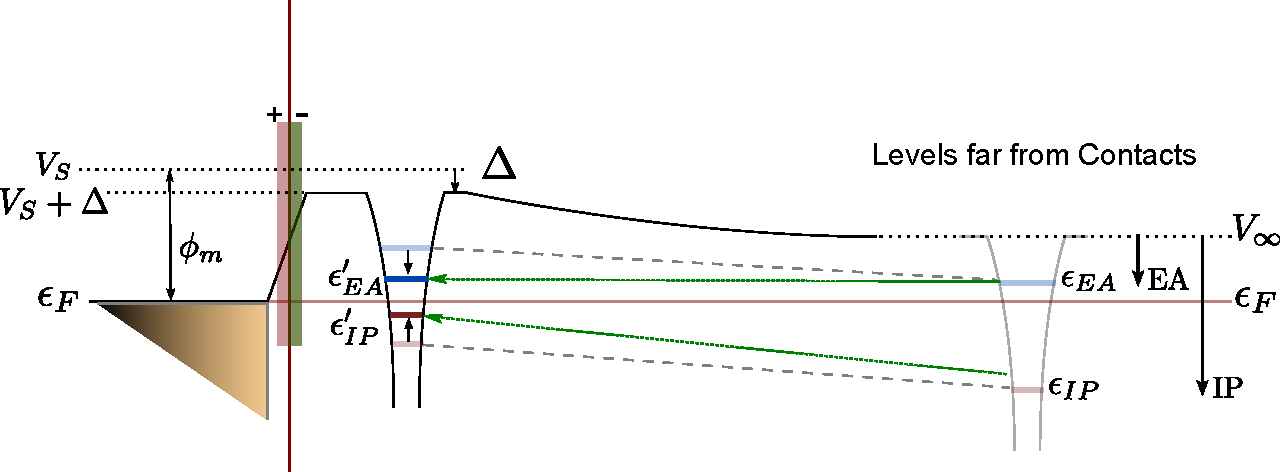
\includegraphics[width=1.2\columnwidth]{img.exp/Illustration/landscape4}\label{fg:shiftstoon0}
   }\\
\subfloat[]{
   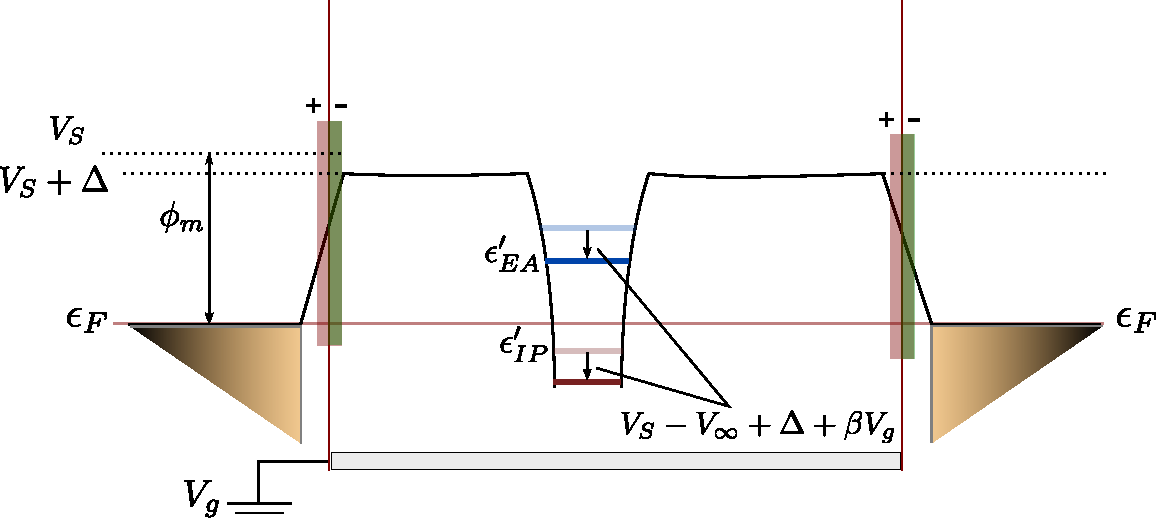
\includegraphics[width=1.0\columnwidth]{img.exp/Illustration/landscape7a}\label{fg:shiftstoon1} 
   }
\subfloat[]{
   \raisebox{.4cm}{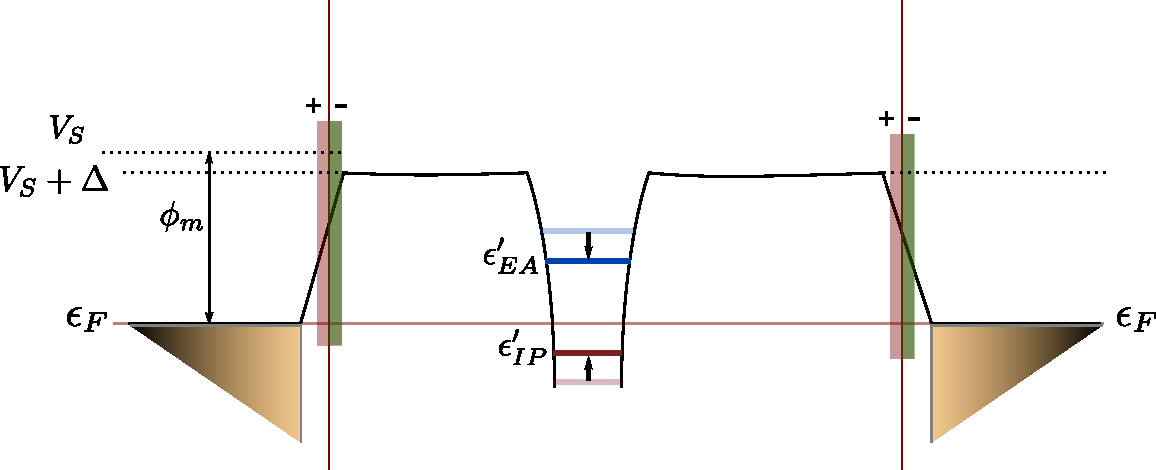
\includegraphics[width=1.0\columnwidth]{img.exp/Illustration/landscape7b}\label{fg:shiftstoon2}} 
   }
\caption{\textbf{Energy landscape during the formation of a metal-molecule interface.} 
(a) Combined rigid and dynamical image-charge effects on molecular levels at a single interface, relative to the molecule in isolation far away. These are a superposition of (b) and (c), where in (b) the surface dipole (shaded red/green) raises the background potential by $V_s-V_\infty$. The static image-charge effect, intrinsic molecular and interface dipoles shift the molecular levels back by $\Delta$, while electrostatic gating shifts by $\beta V_g$. (c) Levels are also subject to renormalization of the gap between the electron affinity $\epsilon_{EA}$ and the ionization potential $\epsilon_{IP}$ levels, where the prime indicates the position after the shift. 
}\label{fg:landscape}
\end{figure*}

We illustrate the most important physical effects as a molecule approaches a clean metal surface in Fig.~\ref{fg:landscape}, following Ishii \etal\cite{Ishii2000} 
The shift of the levels occurring when a molecule is moved towards a metal surface can be divided into two classes. The first type of shift is due to a change 
in the background potential induced by the proximity of the metal and affects all the orbital levels in a similar way. Usually, this is an upward shift. 

The second class of effects are those which shift occupied and unoccupied molecular levels differently, causing the transport gap between them to close (``renormalize'') as the molecule approaches the surface. When combined with the rigid shift, this yields the combined adjustment of levels illustrated in Fig.~\ref{fg:shiftstoon0}. %We discuss these two classes of effects further in the next sections.

\subsection{Background potential effects}

A clean metal surface contains a surface dipole, which is caused by a `spill-out' of the electronic charge density into the vacuum. This dipole has the effect of shifting the chemical potential (just)
outside the surface with respect to the Fermi level inside the metal. Adsorption of a molecule modifies this
dipole.\cite{Seki1997,Ishii1999,Ishii2000,Vazquez2004a,Vazquez2004b} First, if the molecule is physisorbed onto the surface the electron cloud of the molecule will push back the spill-out back (known as the ``push back'' or ``pillow effect'').\cite{Vazquez2007,Flores2009} 
Second, if the molecule is chemisorb rather than physisorb%at the interface
, formation of the bond causes charge transfer, which alters the surface dipole substantially. Third, 
(and most important for %the present
this paper) there is also an image-charge effect, which is generated by the charge distribution of the (possibly neutral) molecule and which  affects all molecular levels.

These effects are combined into a correction $\Delta$ to the background potential shift $V_s$ (which %in principle 
depends on distance), and contribute to a static background potential which raises/lowers the molecular potential-well relative to the gas phase (as in Fig.~\ref{fg:shiftstoon1}). 
This change in background potential is quite similar to the effect of an electrostatic gate field on the molecule, as in three-terminal junctions. 
%In principle DFT captures at least part of this shift, but evaluating the dependence on the molecule-metal separation requires many separate DFT calculations. 
We note that, due to the spatial variation of this potential, different molecular orbitals may shift differently from their gas phase values, but generally the \emph{direction} of these shifts is the same for all, and the differences are rather weak. Therefore, we denote these shifts as 'rigid'.  
 
Oszwaldowski \etal have introduced a many-body method based on DFT\cite{Oszwaldowski2003} for capturing some of this dependence, deriving from dipole and pillow effects. 

The length scale over which the changes to the energy landscape due to a surface dipole layer take place is related to the lateral extent of the surface dipole layer formed at the metal surface. This is typically the scale of the electrode in a mechanically controlled break-junction (MCBJ) experiment, which is of the order of $5$ nm.\footnote{Estimated from the fits of the junction area in Perrin \etal's experiments\cite{Perrin2013}, which fit this as $28$ nm$^2$ and considered the range of $10-50$ nm$^2$ as representative.}
The magnitude of $\Delta$ is suggested by the measurements summarized by Ishii \etal: roughly $0.5-1$ eV, typically a negative correction on an Au substrate. %for H$_2$TPP and ZnTPP films (without thiols).\cite{Ishii1999,Ishii2000} 
Measurements by Koch \etal\cite{Duhm2008,Broker2010,Niederhausen2011} on thin-films with different molecules support these considerations: they find a constant-shift region very near the interface, followed by a linear shift of $\sim1$ eV over a range of roughly $8$\AA\xspace beyond which a regime with constant $\Delta$ sets in.

\subsection{Gap renormalization due to image charges}\label{image_model}

The effects in the preceding section shift all molecular levels in the same direction, in contrast with the closing (``renormalization'') of the energy separation (``gap'') between occupied and unoccupied levels we discuss in this section. 
We are concerned with the chemical potentials associated with charge addition and removal, which are commonly denoted as the electron affinity (EA) and ionization potential (IP). These concepts are well-defined for a gas phase molecule. For a molecule in a transport junction, a similar concept 
can be used provided there is a weak coupling between the molecule and the leads. The EA and IP should be distinguished 
from the highest occupied and lowest unoccupied molecular orbital levels (HOMO and LUMO respectively), as they arise in a DFT calculation.
The difference between the HOMO and the IP is that the latter includes the relaxation effect of the lower-lying orbitals and the leads 
resulting from the removal 
of an electron from the highest occupied level -- a similar difference exists between EA and LUMO. 
In fact, the HOMO and LUMO are the chemical potentials associated with an \emph{infinitesimal} change in the charge on the molecule. The 
IP and EA are defined as the negative of the chemical potential associated with an \emph{integer} charge.
The difference between the EA and IP is
known as the \emph{transport gap}.

In the weak coupling regime, transport can indeed be seen as a succession of steps where an electron is removed (added) to the molecule and then returns to its (approximately) neutral state. As a first approximation, the relaxation of the lower-lying orbitals as a result of changing the charge state of the molecule can be considered to be more or less the same in the gas phase as in a transport junction. The main difference between the two configurations is due to the polarization of the leads, which can be captured effectively by the image-charge effect. This image-charge effect results in a decrease of the transport gap  with decreasing metal-molecule separation, as illustrated in Fig.~\ref{fg:shiftstoon2}. This gap renormalization due to image charges should be contrasted with the rigid shift that was discussed previously. 

It has been extensively discussed in the literature that transport-gap renormalization is due to the image-charge effect,\cite{Quek2007,Neaton2006,Hybertsen1986,Hybertsen2008,Thygesen2009} and the 
polarization response to charge added near a metal surface. It was shown by Neaton \etal\cite{Neaton2006} that for small molecules this potential can be well fitted by an image-potential of the form $-\frac{1}{4z}$ (with $z$ the distance from the plate) beyond the image plane of the metal contact. 
To see in detail how the image-charge effect leads to a reduction of the HOMO-LUMO gap, consider a single point-charge $\delta q=\pm e$ added to a neutral $N$ electron system, near an infinite conducting plate. The charge addition induces an additional energy term $-\frac{\delta q^2}{4z}$, which decreases the ionization potential:
\begin{align}
   \label{eq:HOMO}
   IP\equiv E^{N-1}-E^N \mapsto (E^{N-1}- \frac{\delta q^2}{4z}) - E^N\;,
\end{align}
and \emph{raises} the HOMO-like occupied level $\epsilon_{IP}=-IP$ relative to the vacuum level $V_\infty$. Similarly, it increases the electron affinity:
\begin{align}
   \label{eq:LUMO}
   EA \equiv E^{N}-E^{N+1} \mapsto E^{N} -(E^{N+1}- \frac{\delta q^2}{4z})\;,
\end{align}
and \emph{lowers} the LUMO-like unoccupied level $\epsilon_{EA}=-EA$ relative to the vacuum level $V_\infty$. Together, these effects renormalize the transport gap 
\begin{align}
   \label{eq:GAP-RENORMA}
IP-EA = E^{N+1} + E^{N-1} - 2E^{N} -2\frac{e^2}{4z}.
\end{align}

These effects are important in many nanoscale molecular systems, as has been argued on both experimental\cite{Kubatkin2003,Hedegaard2005,Bruot2012} and theoretical grounds \cite{Neaton2006,Quek2007,Mowbray2008,Kaasbjerg2008,Hybertsen2008,Thygesen2009} and are crucial for understanding and designing future molecular devices.

\subsection{Limitations of DFT}

%DFT is the workhorse of quantum-chemistry calculations.\cite{Burke2012} 
In transport calculations, DFT is often combined with the non-equilibrium Green's function (NEGF) method, in order to describe a molecule (and, in most cases, part of the metal electrodes) embedded between semi-infinite metal leads as an open system.\cite{Brandbyge2002,Stokbro2003a,Rocha2006,Evers2006,Verzijl2012}
The DFT calculation involves the calculation of the Hartree potential, which takes static polarization into account. However, it does not describe polarization effects induced by changes in the charge distribution that occur in transport. Together with the presence of spurious self-interactions,\cite{Perdew1981} this shortcoming is responsible for the incorrect predictions for one- and two-particle excitations (band gaps and exciton energies, respectively). This can also be formulated in terms of a lack of a correct derivative discontinuity in the DFT functional.\cite{Perdew1982,Perdew1983} 

In weakly coupled systems, where the (integer) charge fluctuations are substantial, these shortcomings become apparent. In this limit, transport is dominated by a set of transporting levels which correspond to transitions between many-body states of the isolated molecule. These transitions show up as peaks in the spectral density, with a width determined by the coupling to the leads. If the molecule is (approximately) neutral at zero bias, the HOMO and LUMO orbitals are the main candidate channels for low-bias transport. 

In the gas phase, the difference between the HOMO (LUMO) and the IP (EA), can easily be obtained as the difference between the DFT orbital levels and the corresponding chemical potentials from $\Delta$SCF calculations.\cite{Jones1989} Neaton \etal\cite{Neaton2006} have suggested that these differences are similar for the molecule in the junction, which leads to the so-called `scissors-operator' procedure, where the positions of the transmission peaks corresponding to HOMO and LUMO are corrected by an amount obtained from gas phase. 

The polarization effects due to the contacts give an additional difference between gas phase and junction, and it is these last effects that we focus on. Kaasbjerg and Flensberg\cite{Kaasbjerg2008} and Mowbray \etal\cite{Mowbray2008} have shown that these affect the calculated transport gap significantly, which together with the scissors operator bring it into much better agreement with experimental observations, particularly when a gate is present (which provides additional screening).\cite{Kaasbjerg2008}

Since good ground-state charge distributions are obtained using DFT for a given charge state, we show how to incorporate these into an appropriate generalization of Eq.~\eqref{eq:HOMO}-\eqref{eq:LUMO}.

\subsection{Full Image-Charge Effect Model}\label{full_model}

\begin{figure}
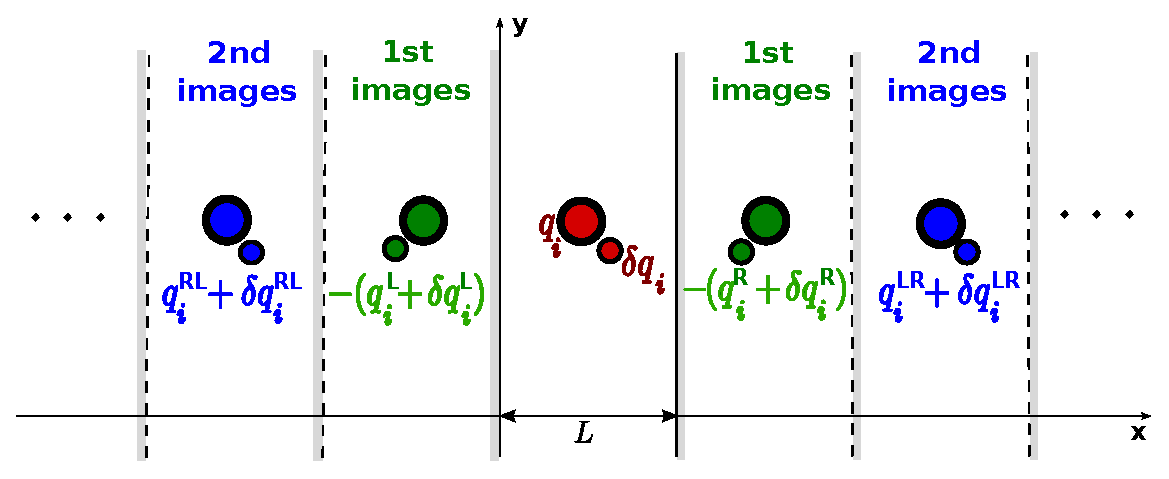
\includegraphics[width=\columnwidth]{img.exp/Illustration/mirrorplanes}
\caption{Point charges between parallel plates, leading to an infinite series of image charges (first set of images in green, second set (images of images) in blue, \emph{etc}). Note the $\delta q_i$ added to the charges $q_i$ of the $N^\text{th}$ charge state, in going to the $(N+1)^\text{st}$ charge state: these also induce a series of repeated images.}\label{fg:imagemodel}
\end{figure}

Following Kaasbjerg and Flensberg,\cite{Kaasbjerg2008} and Mowbray \etal\cite{Mowbray2008}, we simplify the image-charge effects for the full spatial charge density by considering atomic point charges.
These are calculated from the charge states with $N-1$, $N$ (neutral) and $N+1$ electrons on the molecule. The atomic charges are denoted $q_j$, and are located at ${\bm r}_j$. The images of the atomic charges are denoted as $q^I_j$, 
%the first image has charge $q^I_j= -q_j$, the second $q^I_j = q_j$ and so on.
and are located at ${\bm r}^I_j$; this position is found by (multiple) reflection with respect to the image planes.%which are located just outside the plane passing through the outer atomic surfaces.
\cite{Smith1989,Quek2007} When the total charge on the molecule changes, the atomic charges change by $\delta q_j$, inducing additional image charges $\delta q^I_j$. The correction to a molecular level for a change in the charge state is then:
\begin{align}
\label{eq:JT}
\Delta = \sum_{i, j} \frac{\delta q_i q_j^I}{\rijI}
+ \sum_{i,j} \frac{\delta q_i \delta q_j^I}{\rijI} + U_\text{self}(\delta q_i)\;.
\end{align}

%where we collect all the effects not depending on the molecule-metal separation into the term $U_\txt{self}$.
Eq.~\eqref{eq:JT} can be derived by considering the work involved in assembling the point-charge configuration.
The superscript $I$ implies a summation over the images. % a single image for the single-plane case, and an infinite series for  planes which face and mirror each other, as shown in Fig.~\ref{fg:imagemodel}.
The first term is linear in the $\delta q_i$ and it represents the interaction between this added charge and the images $q^I_j$ of the reference configuration, this term affects the (constant) level shift.
The second term is quadratic in the $\delta q_j$ and it contains the interaction between the added charges and their images $\delta q^I_j$, and it is responsible for the gap renormalization. The last term collects the effects not depending on the molecule-metal separation. 
%The first term affects the (constant) level shift 
%\[
%\Delta = \sum_i \frac{q_i^I}{|{\bm r}_i^I - {\bm r}|}
%\] 
%whereas the second term is responsible for the gap renormalization. 

When there is only one plane, and we neglect the self-interaction, the image-charge effect reduces to:
\[
\Delta_\text{ICE} = - \frac{2q\,\delta q + \delta q^2}{4z}\;,
\]
where we recognize the extra term representing background potential shift compared with Eq.~\eqref{eq:HOMO}. %Note that for an uncoupled point-like system, $q=0$, so in that case there is no contribution to the background potential.

%To evaluate this model, we need the atomic charges for different molecular charge states. Due to their nature as spatial decompositions, we prefer Hirshfeld or Voronoi decompositions over the basis-set decomposition involved in Mulliken decompositions. 
The core of this method is to perform the image charge calculation using atomic charges calculated for the molecule \emph{inside the junction} (due to their nature as spatial decompositions, we prefer Hirshfeld or Voronoi decompositions over the basis-set decomposition involved in Mulliken decompositions) and compare the results with those based on the gas phase, as was done in the literature \cite{Mowbray2008,Hybertsen1986,Quek2007}.
%as was done by Mowbray \etal,\cite{Mowbray2008} with the additional assumption motivated by Hybertsen \etal\cite{Hybertsen1986} and Neaton \etal\cite{Quek2007} that taking only the atomic charges associated with IP already captures the image effects for both occupied and unoccupied levels. 
Finally, we find the image-charge corrections to the occupied and unoccupied levels respectively for varying molecule-electrode distance.

To obtain the atomic charge distributions for different charge states of the molecule inside the junction, we use constrained density functional theory (CDFT). In CDFT, the minimum of the energy functional is searched under the constraint that the integral
$\int f(\bfr) n(\bfr) \; d^3 r,$ has a pre-defined value. $f(\bfr)$ is a given function and $n(\bfr)$ is the electron density. 
We take $f(\bfr)$ to be 1 on the molecule, and 0 outside.
%We start from a well-defined equilibrium state, defined by the junction at zero bias and gate voltage. The molecule is then approximately (but not exactly) neutral. Note that by `molecule', we mean the set of atoms that are most weakly coupled to the environment -- it is therefore necessary to identify the weakest coupling in the junction. We shall try different partitionings for the junctions studied in this paper.

The constraint is ensured through a Lagrange parameter $V$ and is translated in to a term $Vf(\bfr)$ added to the potential. This extra potential, which is equivalent to a gate voltage, has been implemented in our transport code %(it is equivalent to a gate voltage)
and it can %thus 
be used to 
%perform a CDFT calculation 
enforce one extra (one less) electron on the molecule in comparison with the reference state% defined by the junction at zero bias and gate voltage
. 

In section~\ref{Sec:BDA}, we shall apply our method to a standard molecule and compare our results with those in the literature.
In section \ref{Sec:ZnTPP} we apply our method for Zn-porphyrins, for which Perrin \etal performed  single-molecule experiments, and argue that the extra physics captured in %the second 
our approach is essential for understanding the transport experiments.



\section{Image charge effects for benzenediamine (BDA)} \label{Sec:BDA}

%There is evidence that metal-molecule-metal junctions, formed by Au point contacts, exhibit reproducible conductance values when amine groups rather than thiols or isonitriles are used to attach the molecules to the junction contacts \cite{Venkataraman2006}. The reason is that 
The amine-Au bonding motif besides being weak compared with thiols or isonitriles \cite{Hakkinen2012}, is also well-defined and flexible, so that measurements on transport properties are less affected by changes in local structure in the contacts \cite{Venkataraman2006,Quek2007,Venkataraman2007}. Junctions with amine groups therefore allow for comparisons of calculated and measured transport properties.

For isolated molecules, the electronic structure is described in terms of molecular orbitals. However, the concept of molecular orbitals is no longer strictly valid when we consider metal-molecule-metal junctions, as hybridization effects broaden the levels into resonances. One way of generalizing the orbital concept is to consider the projection of the Hamiltonian of the contacted system onto the subspace spanned by the basis functions of the molecule. The eigenstates of the projection, called transport orbitals, can be viewed as molecular orbitals renormalized by the electrodes. For weakly coupled molecules, these can be related to the unrenormalized molecular orbitals, the amine-gold bond is an example we can work in detail.



%\subsection{BDA Electronic Structure}\label{BDA electronic_structure}

We first consider %the electronic structure of 
the 1-4 Benzenediamine molecule in gas phase and a Au-BDA-Au fragment, see Figs. \ref{BDA-gas-phase} and \ref{BDA-fragment}. For each of these we analyze the orbitals near the Fermi energy of the Au electrodes, which are expected to be most relevant for transport. The electronic structure for the gas phase and the fragment are shown in Figs. \ref{fg:BDA-gas} and \ref{fg:BDA-frag} respectively.

\begin{figure}
\subfloat[BDA Gas-Phase Geometry]{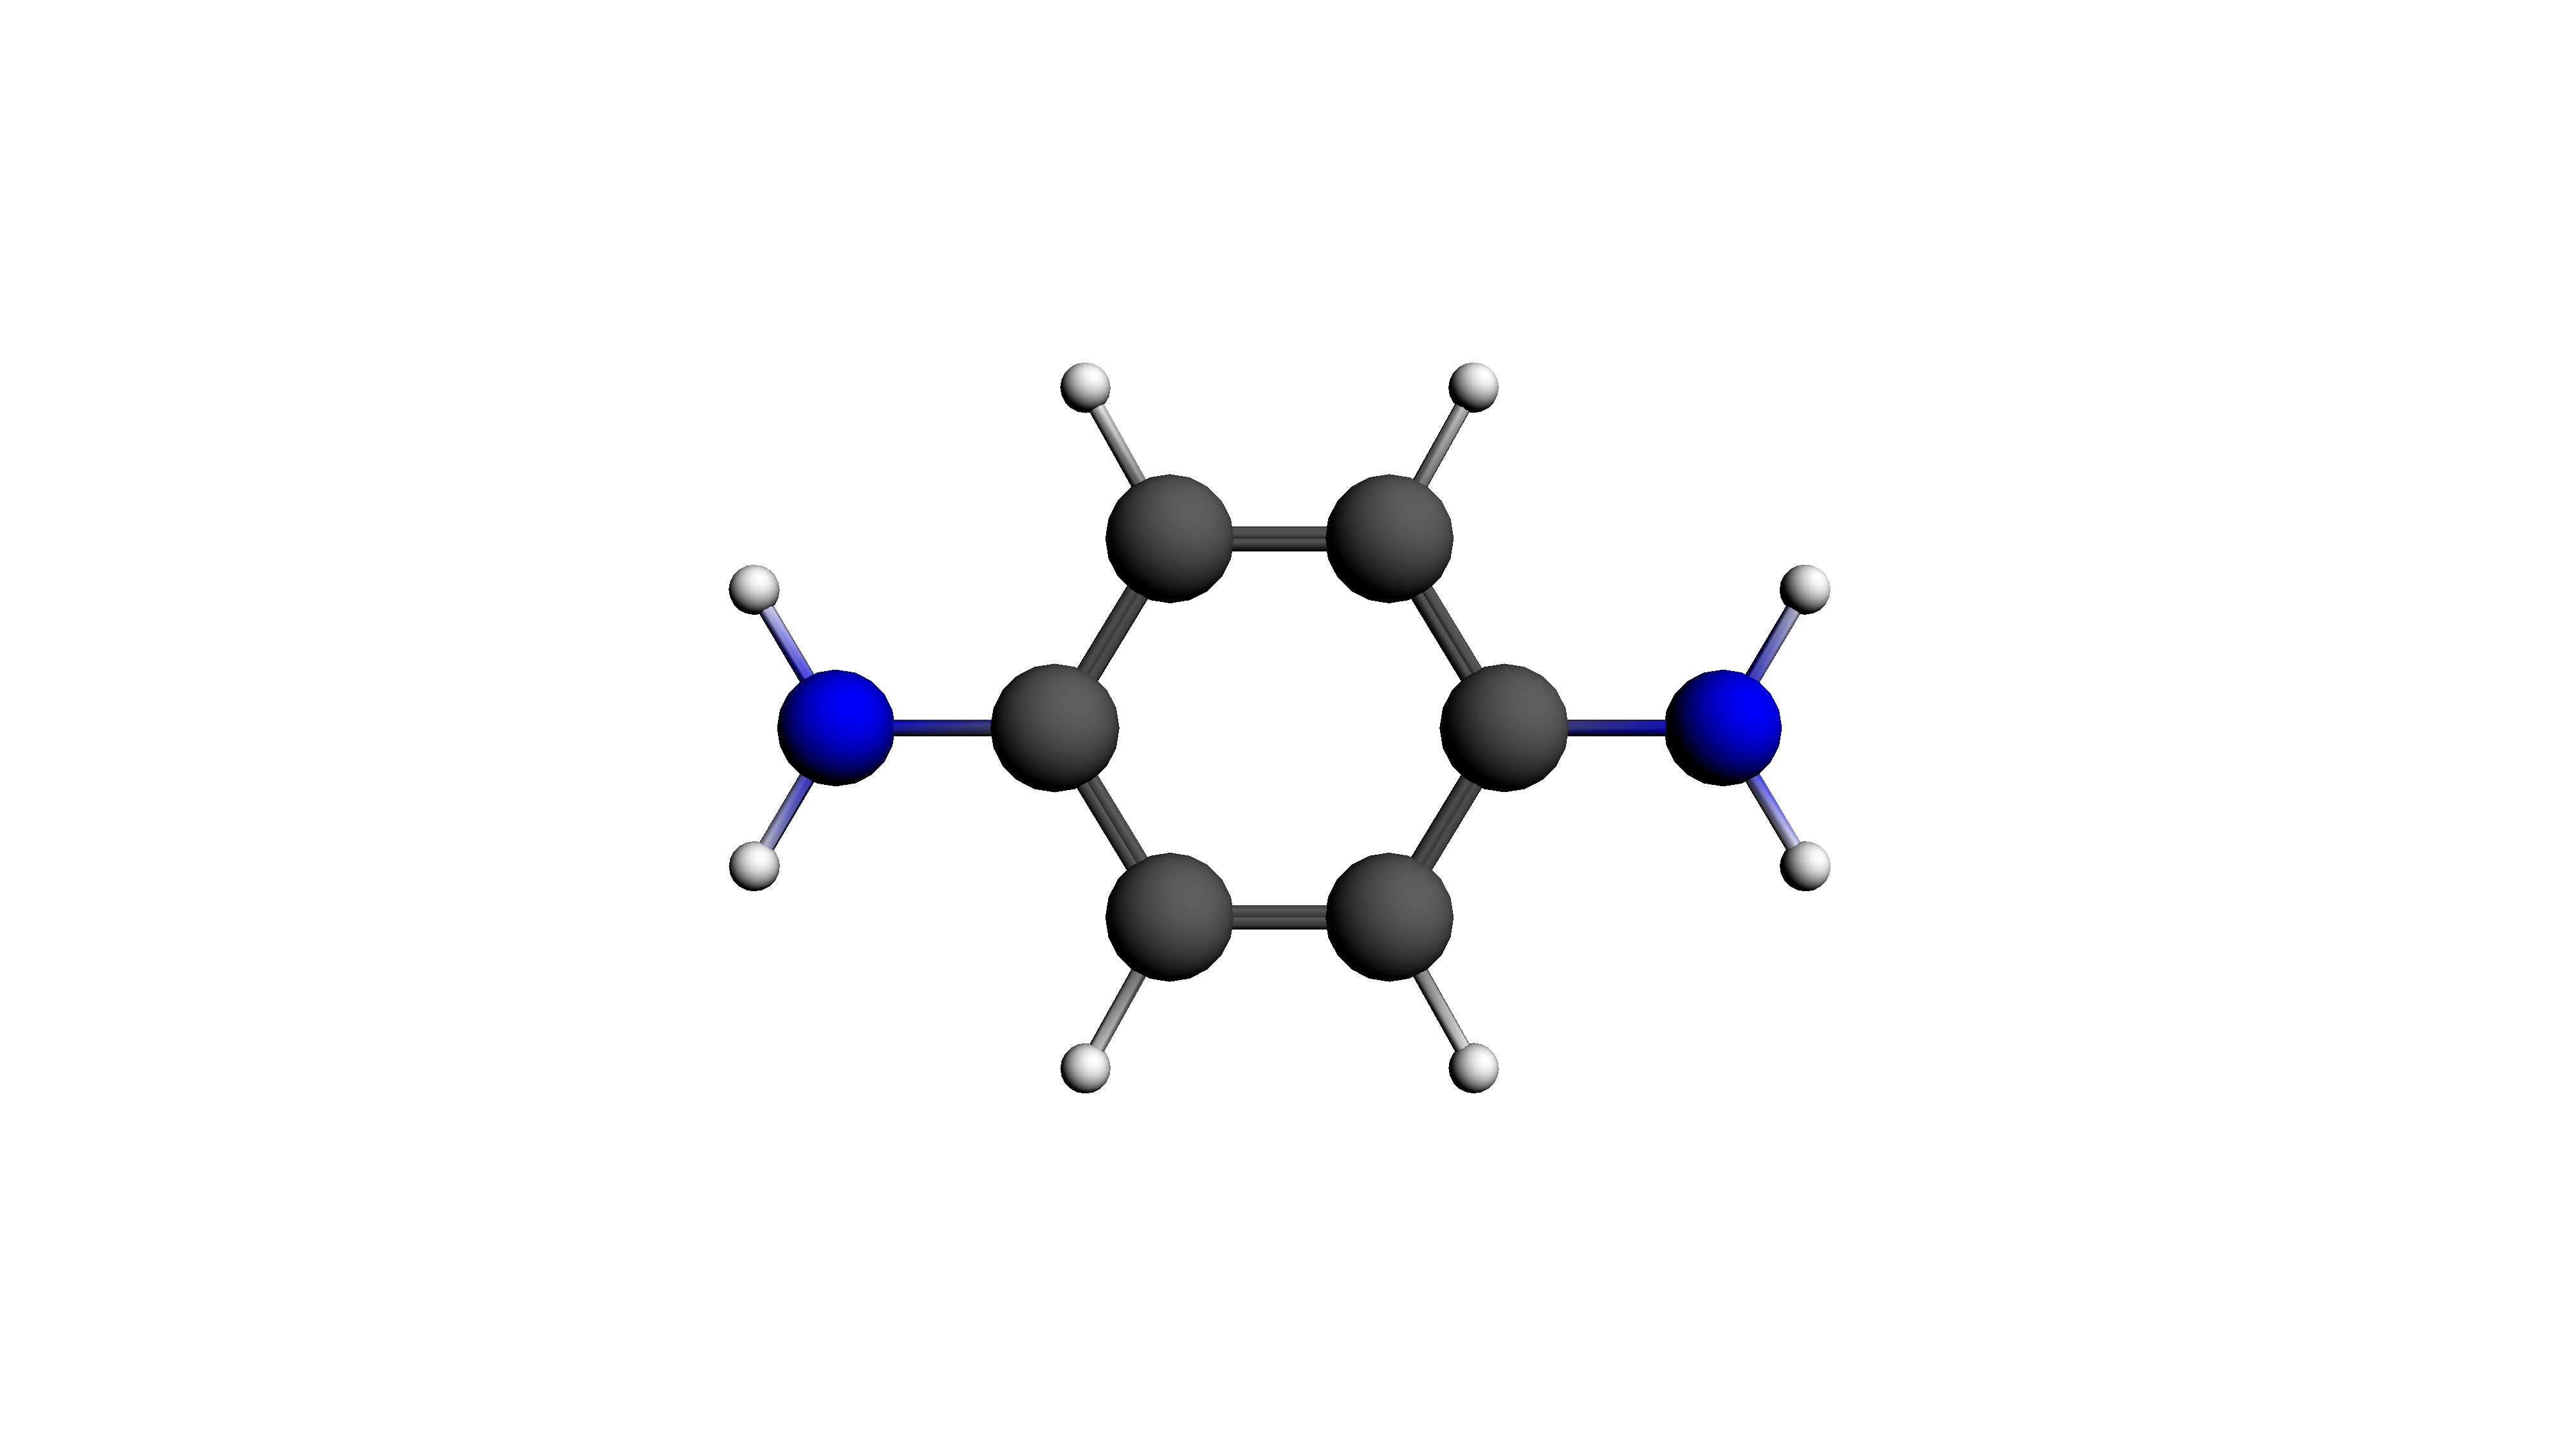
\includegraphics[width=.475\columnwidth]{img.exp/Fragment-geoms/BDA-fragment}\label{BDA-gas-phase}}\hfill
\subfloat[Au-BDA Fragment Geometry]{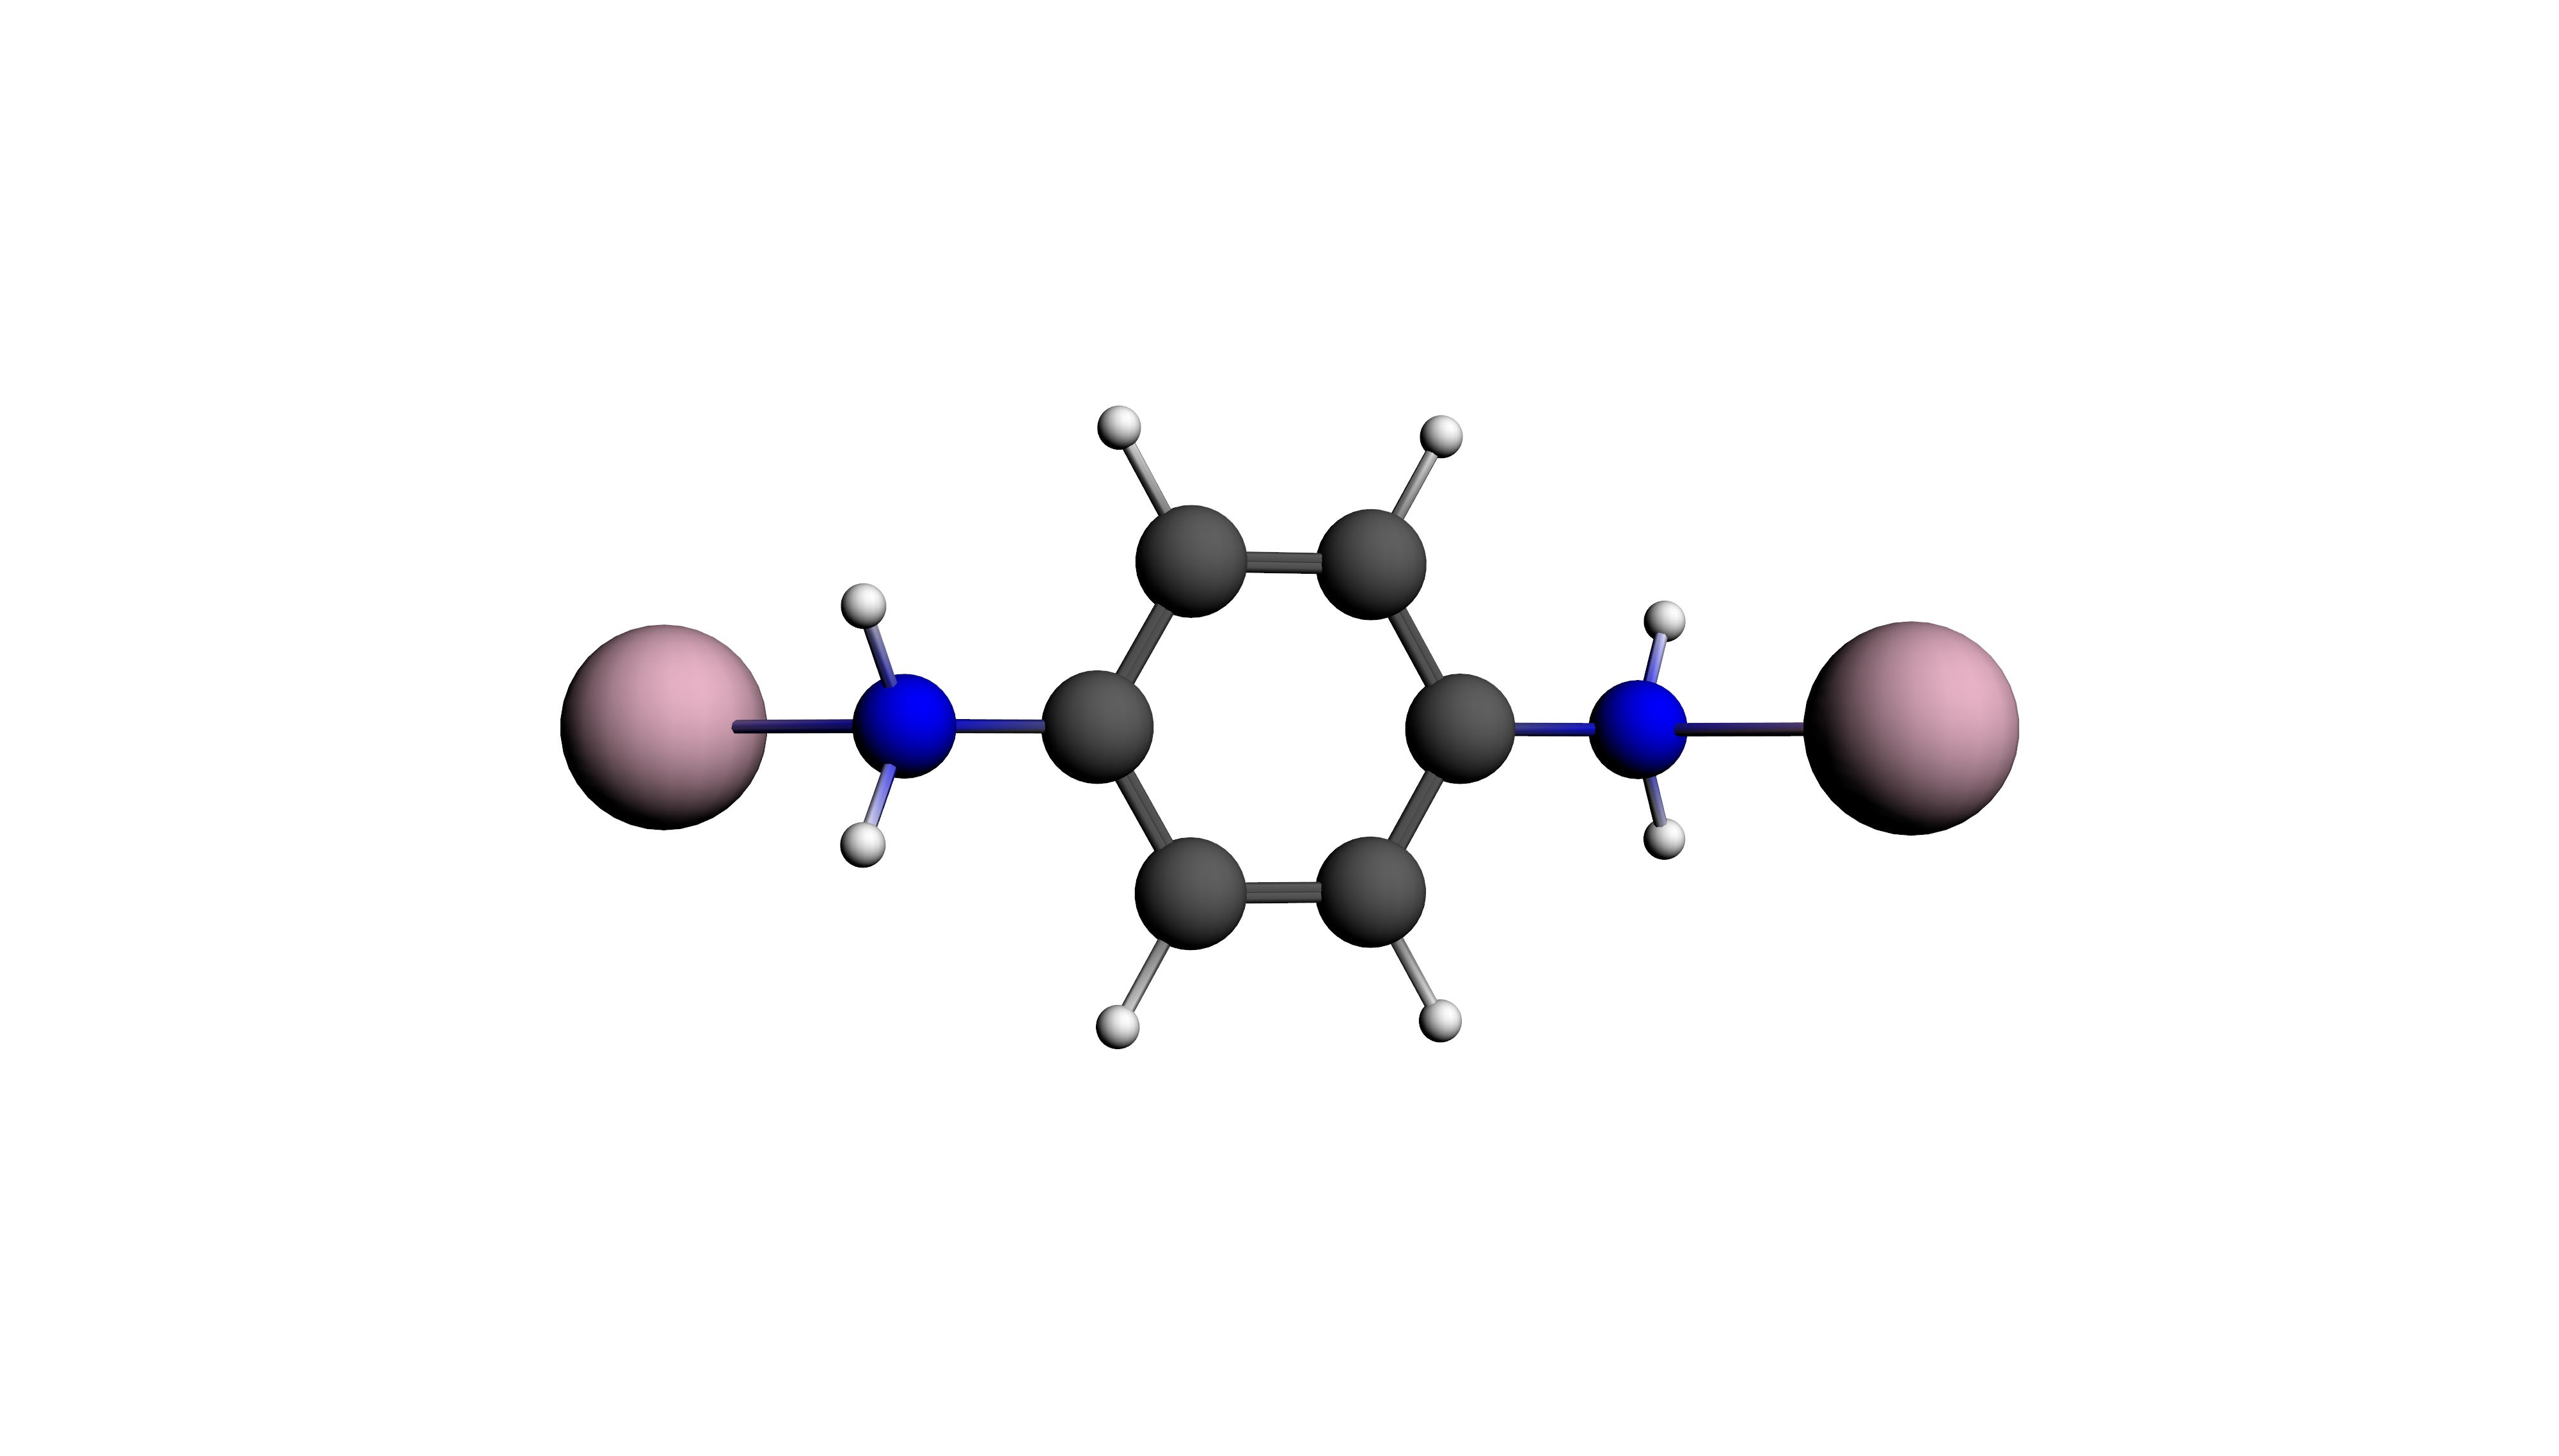
\includegraphics[width=.525\columnwidth]{img.exp/Fragment-geoms/BDA-fragment-au}\label{BDA-fragment}}\\
\subfloat[Au-BDA Junction Geometry]{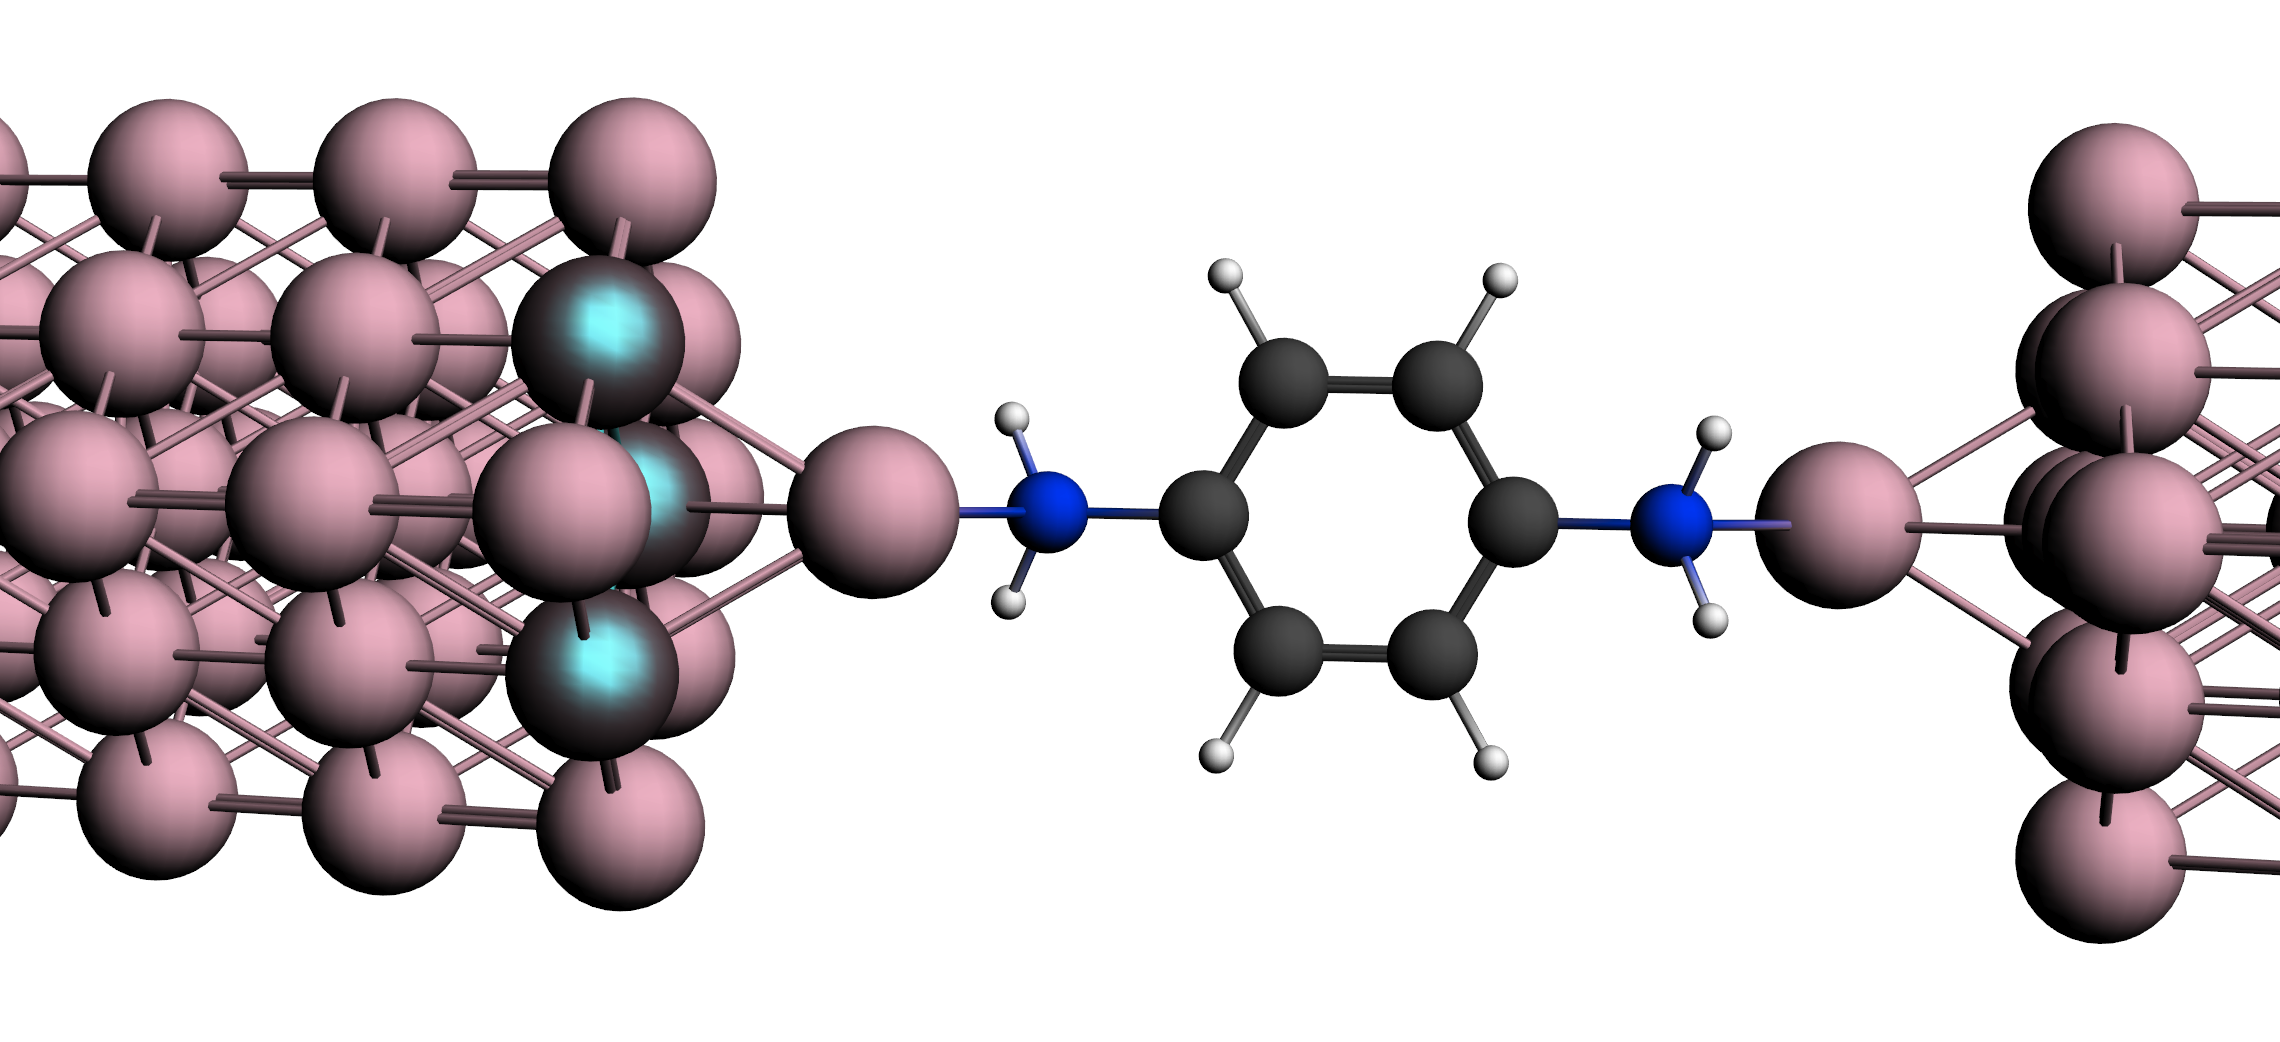
\includegraphics[width=.85\columnwidth]{img.exp/BDA-binding1} \label{BDA-binding}}
\caption{Geometries of BDA in (a) gas phase and (b) as a fragment. (c) (I,I) junction geometry. Metal ions are pink-grey, the blue-gray atoms are the substrate atoms coupled to the protruding gold atom. Left and right Au atoms show placement relative to a (111) surface.} \label{fg:3BDAgeometries}
\end{figure}

\begin{figure}
\subfloat[LUMO+1]{ 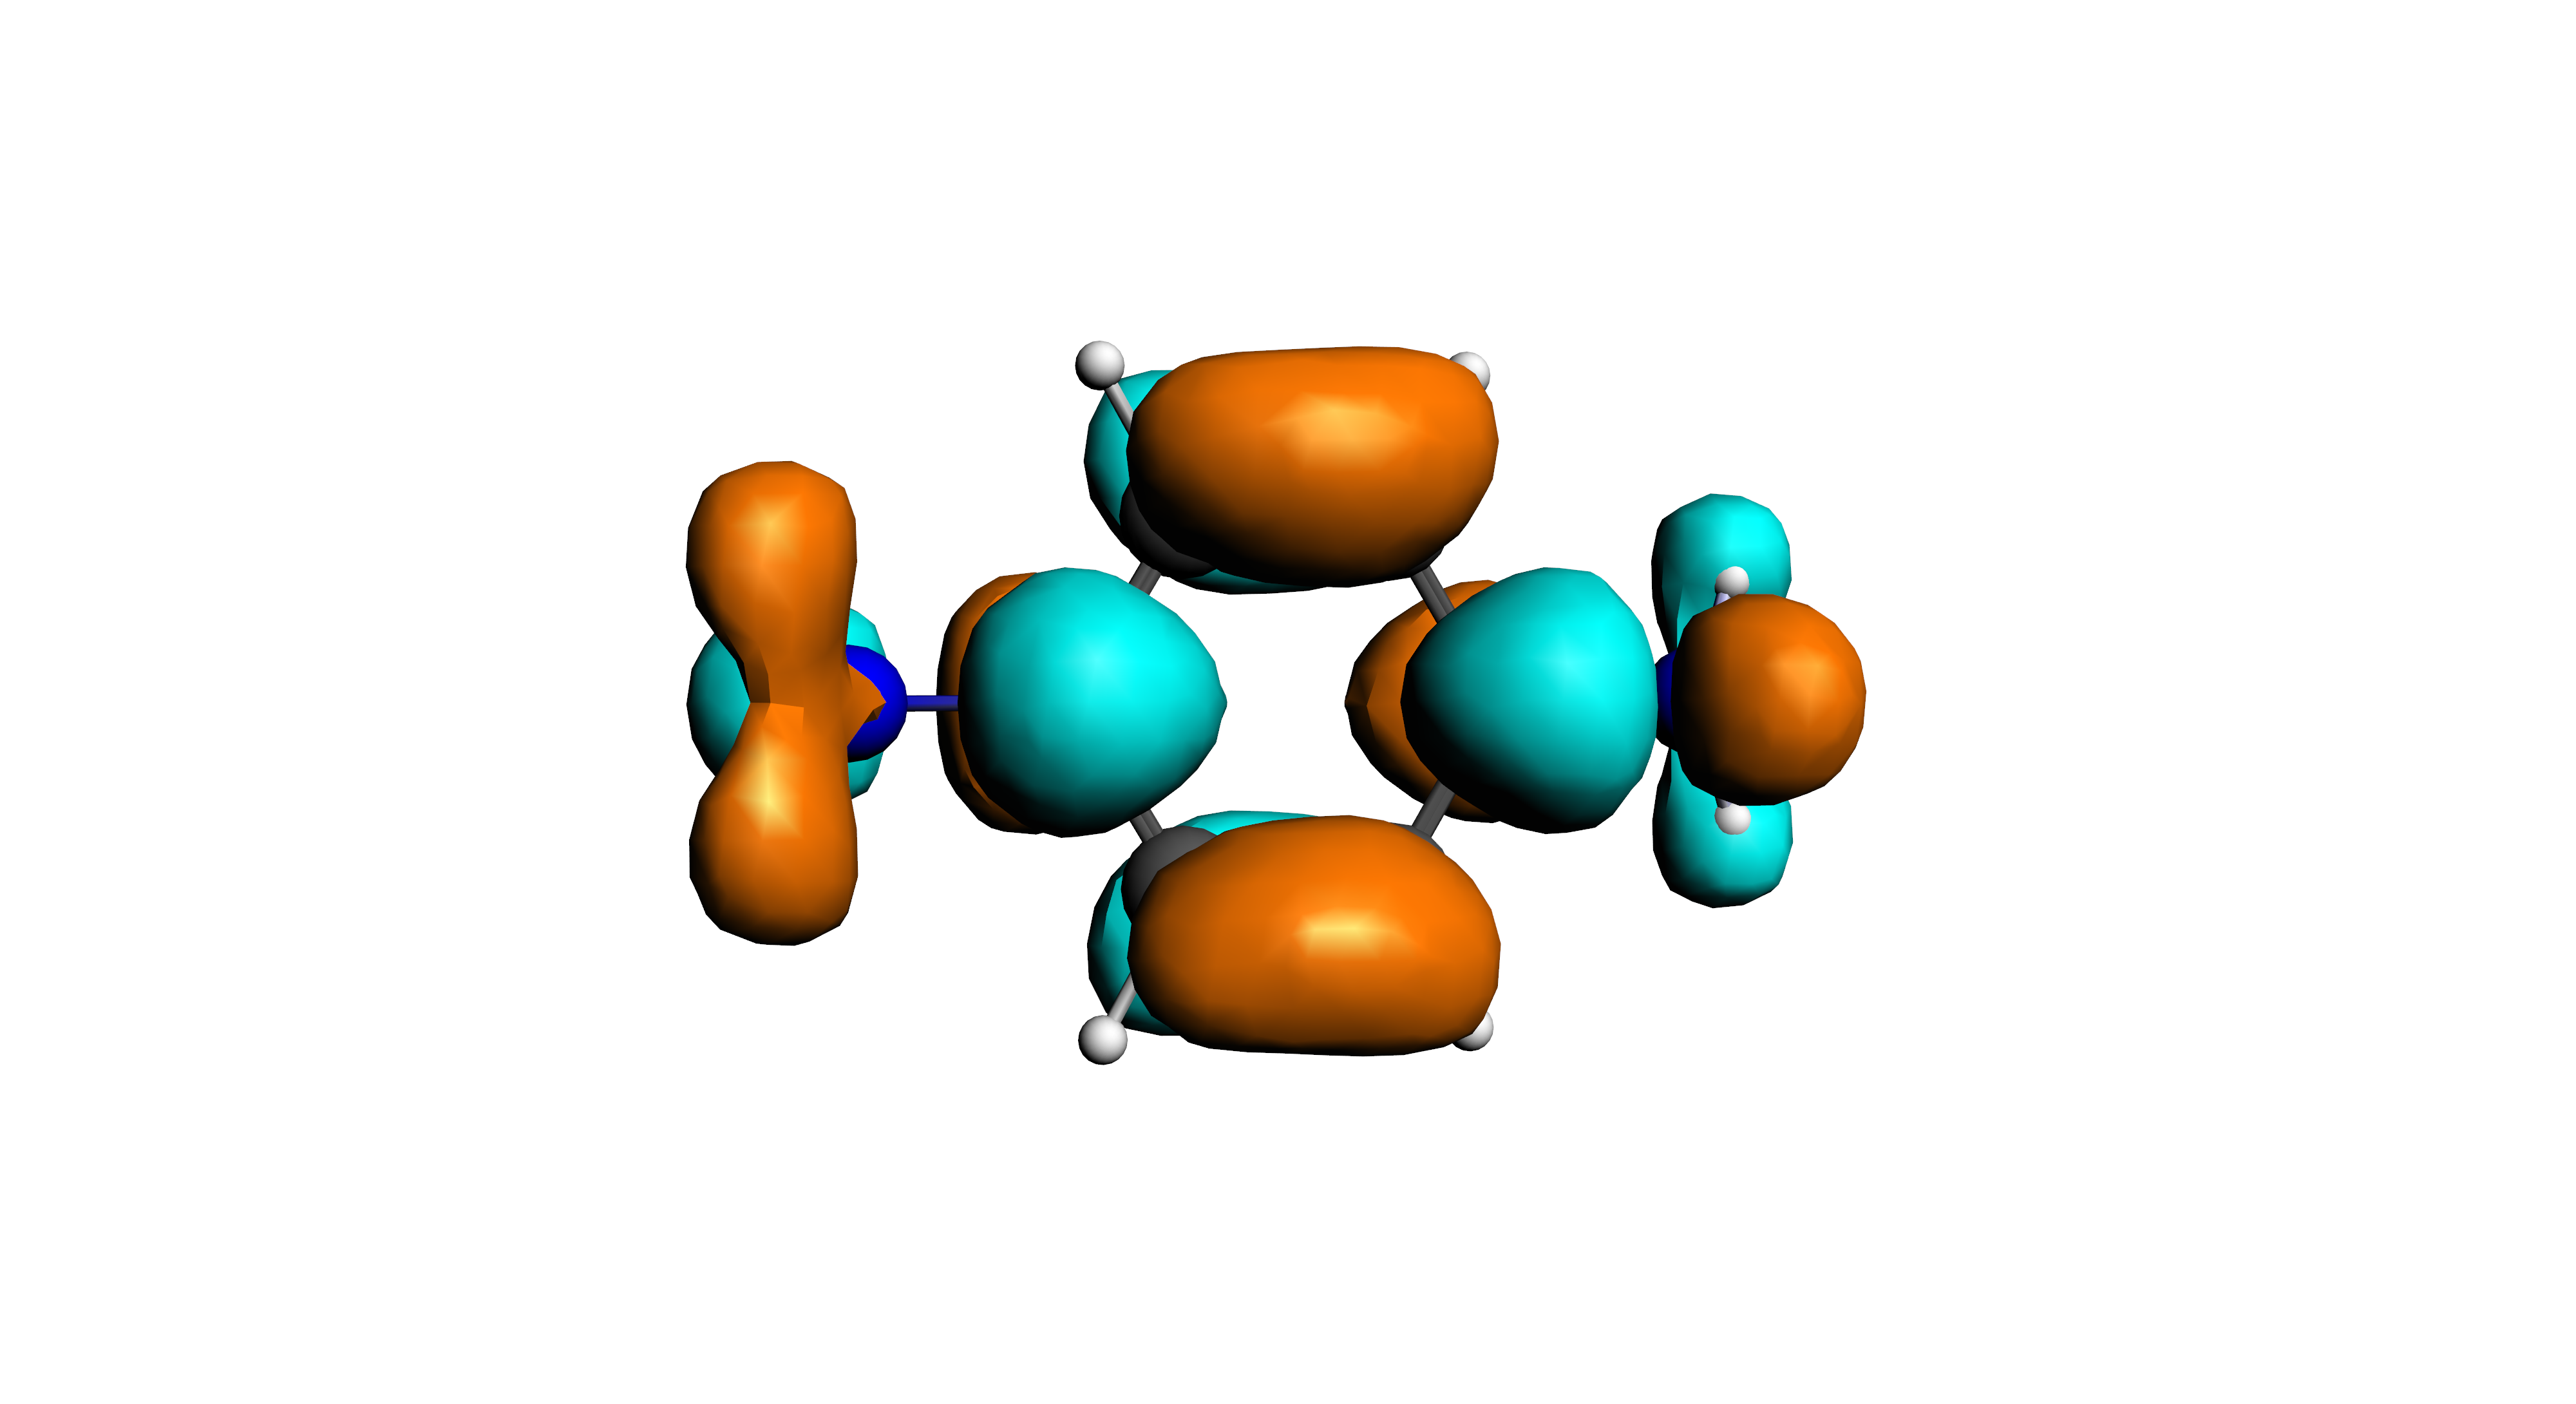
\includegraphics[width=.5\columnwidth]{img.exp/BDA-Levels/gas-phase/LUMO+1.png} }
\subfloat[LUMO]{ 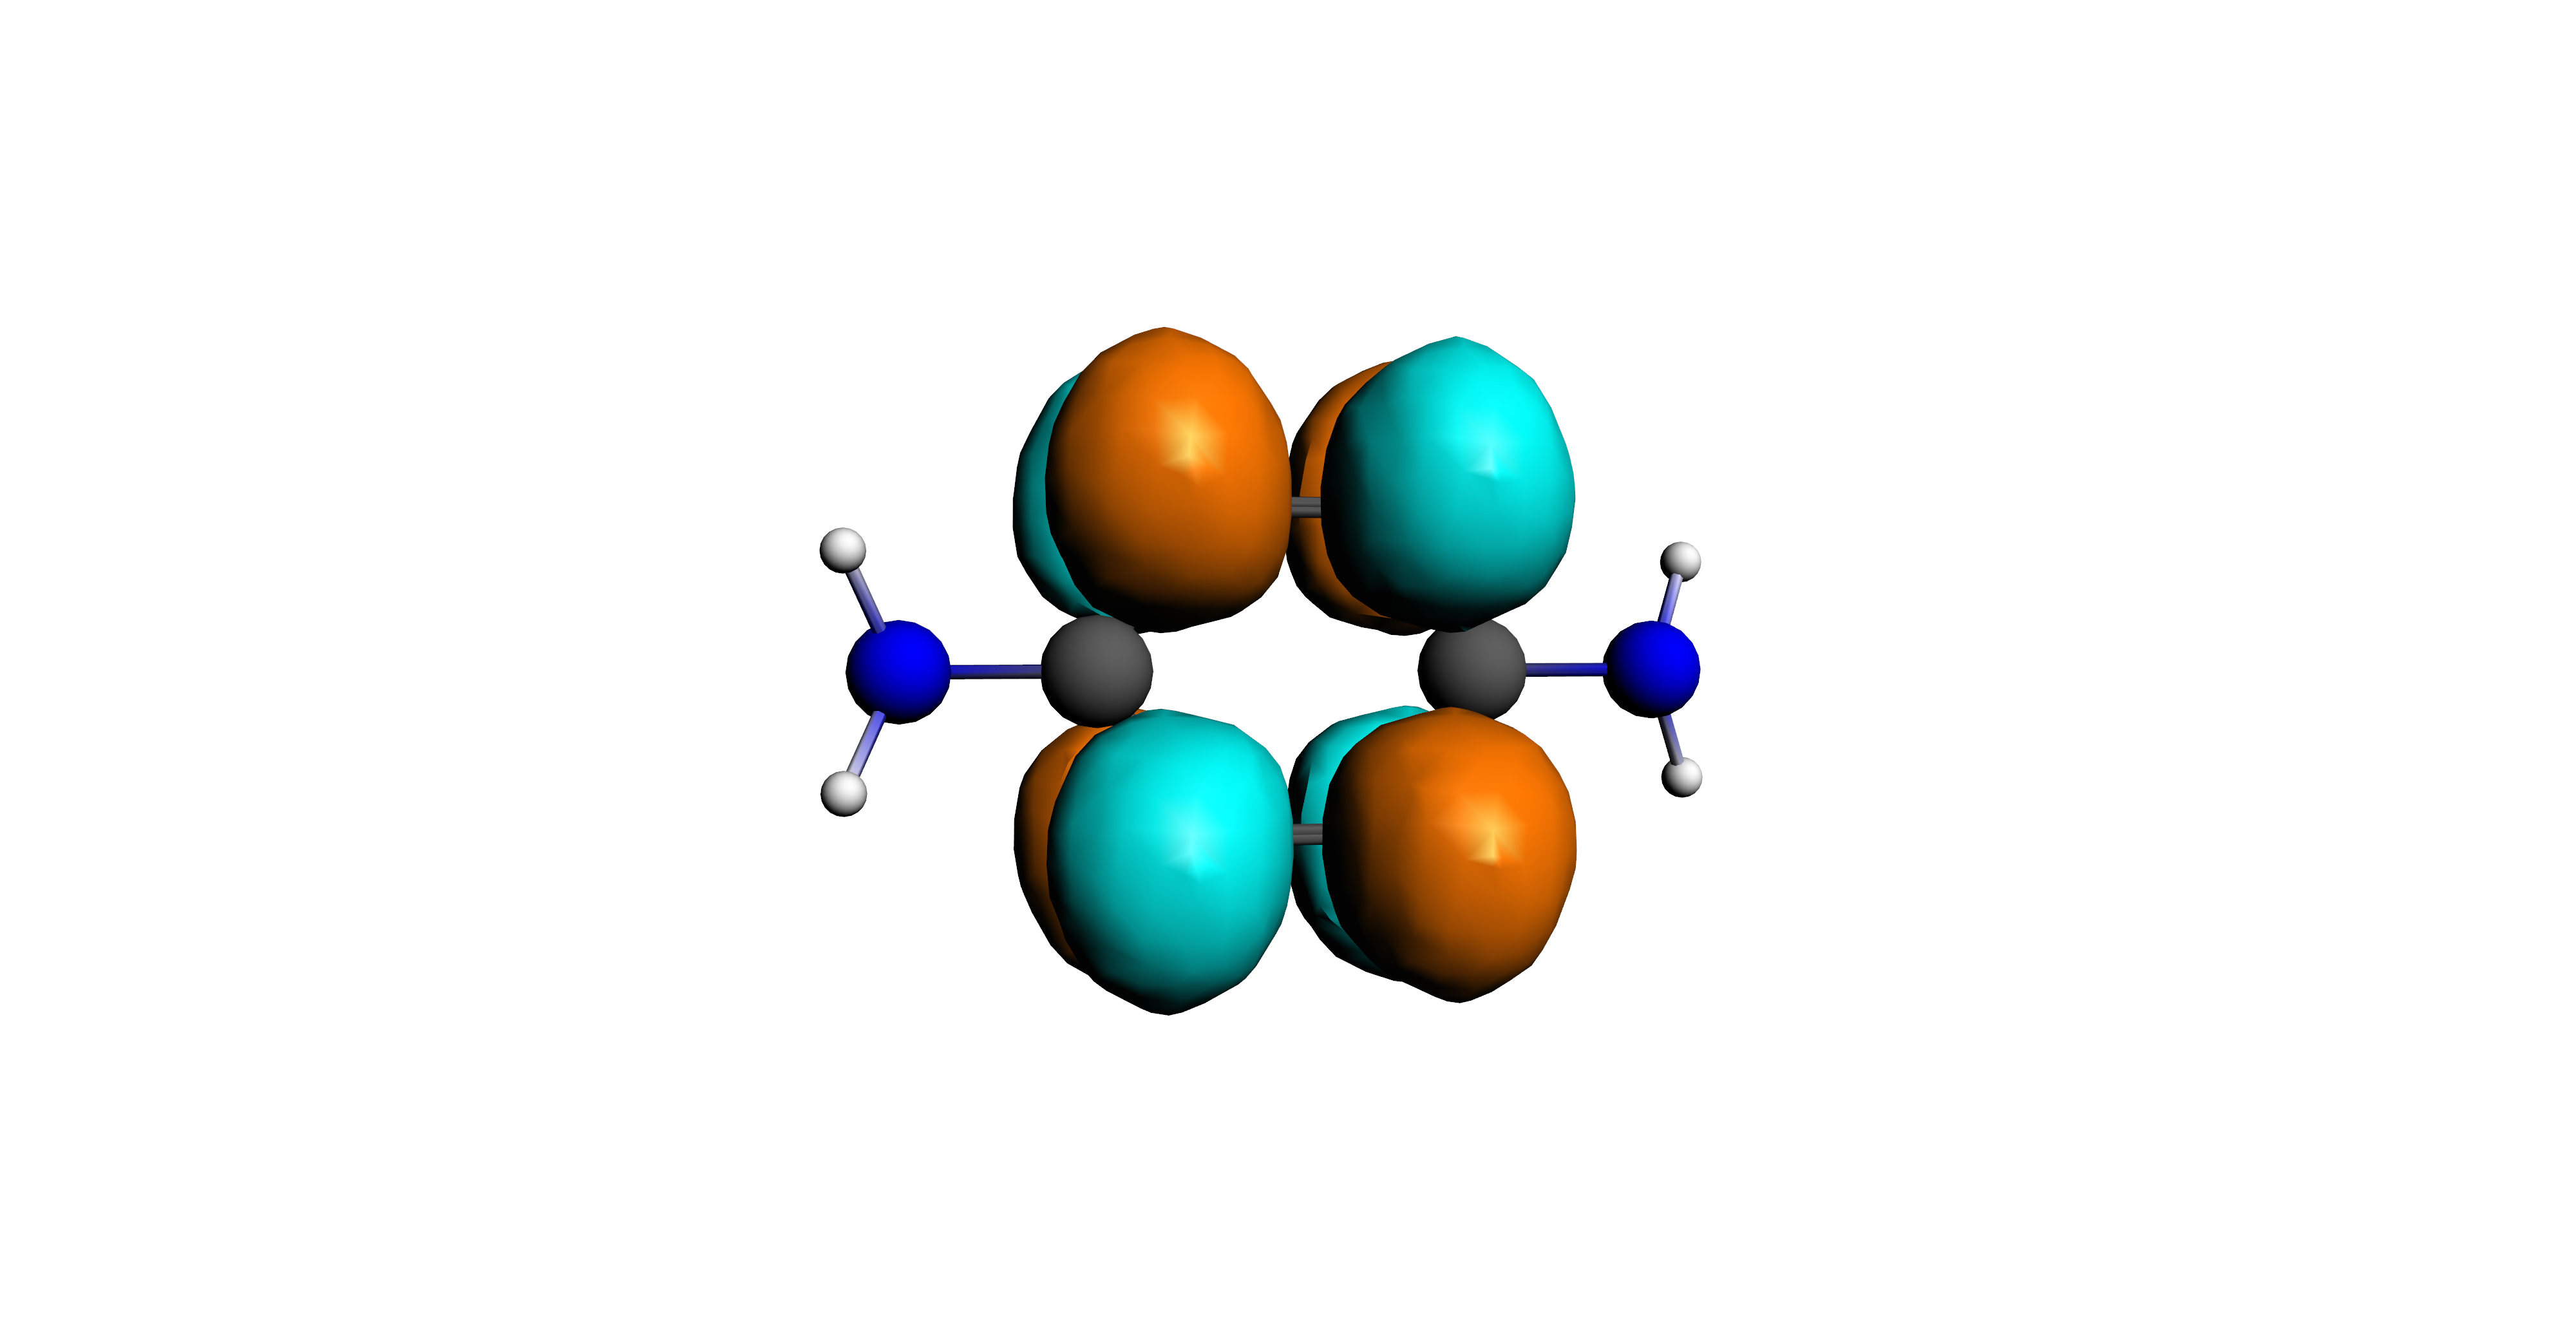
\includegraphics[width=.5\columnwidth]{img.exp/BDA-Levels/gas-phase/LUMO.png} }\\
\subfloat[HOMO]{ 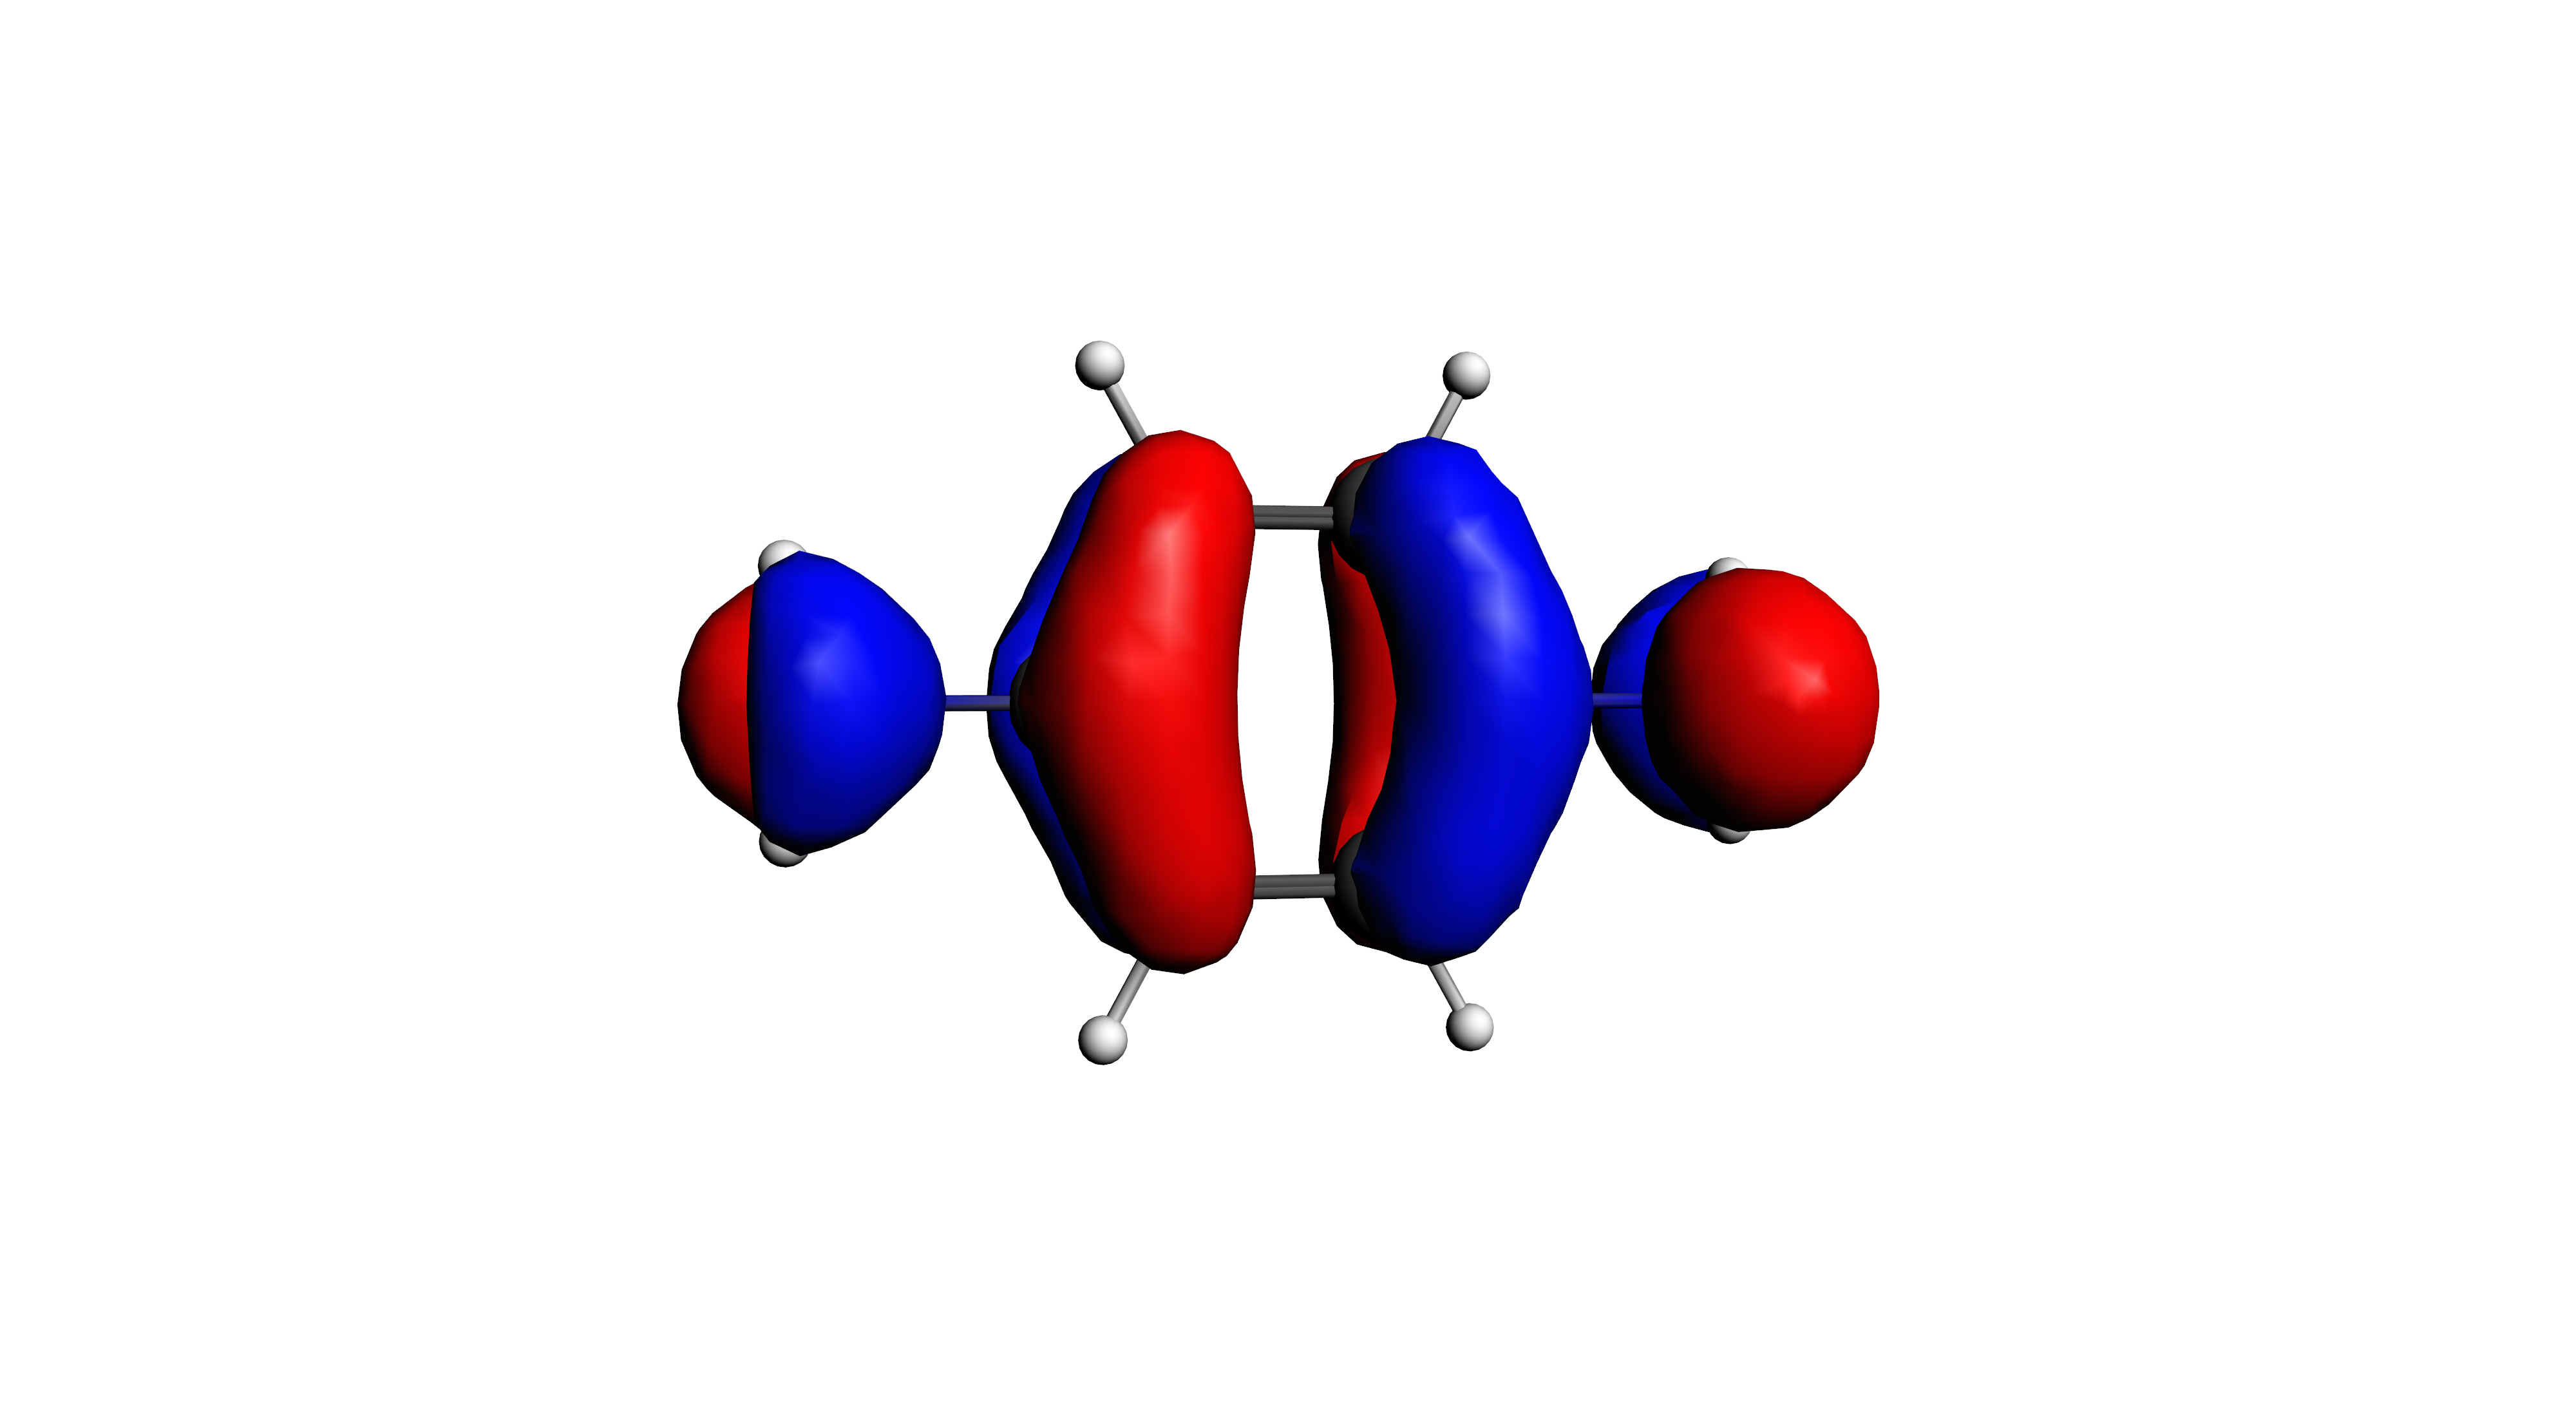
\includegraphics[width=.5\columnwidth]{img.exp/BDA-Levels/gas-phase/HOMO.png} }
\subfloat[HOMO-1]{ 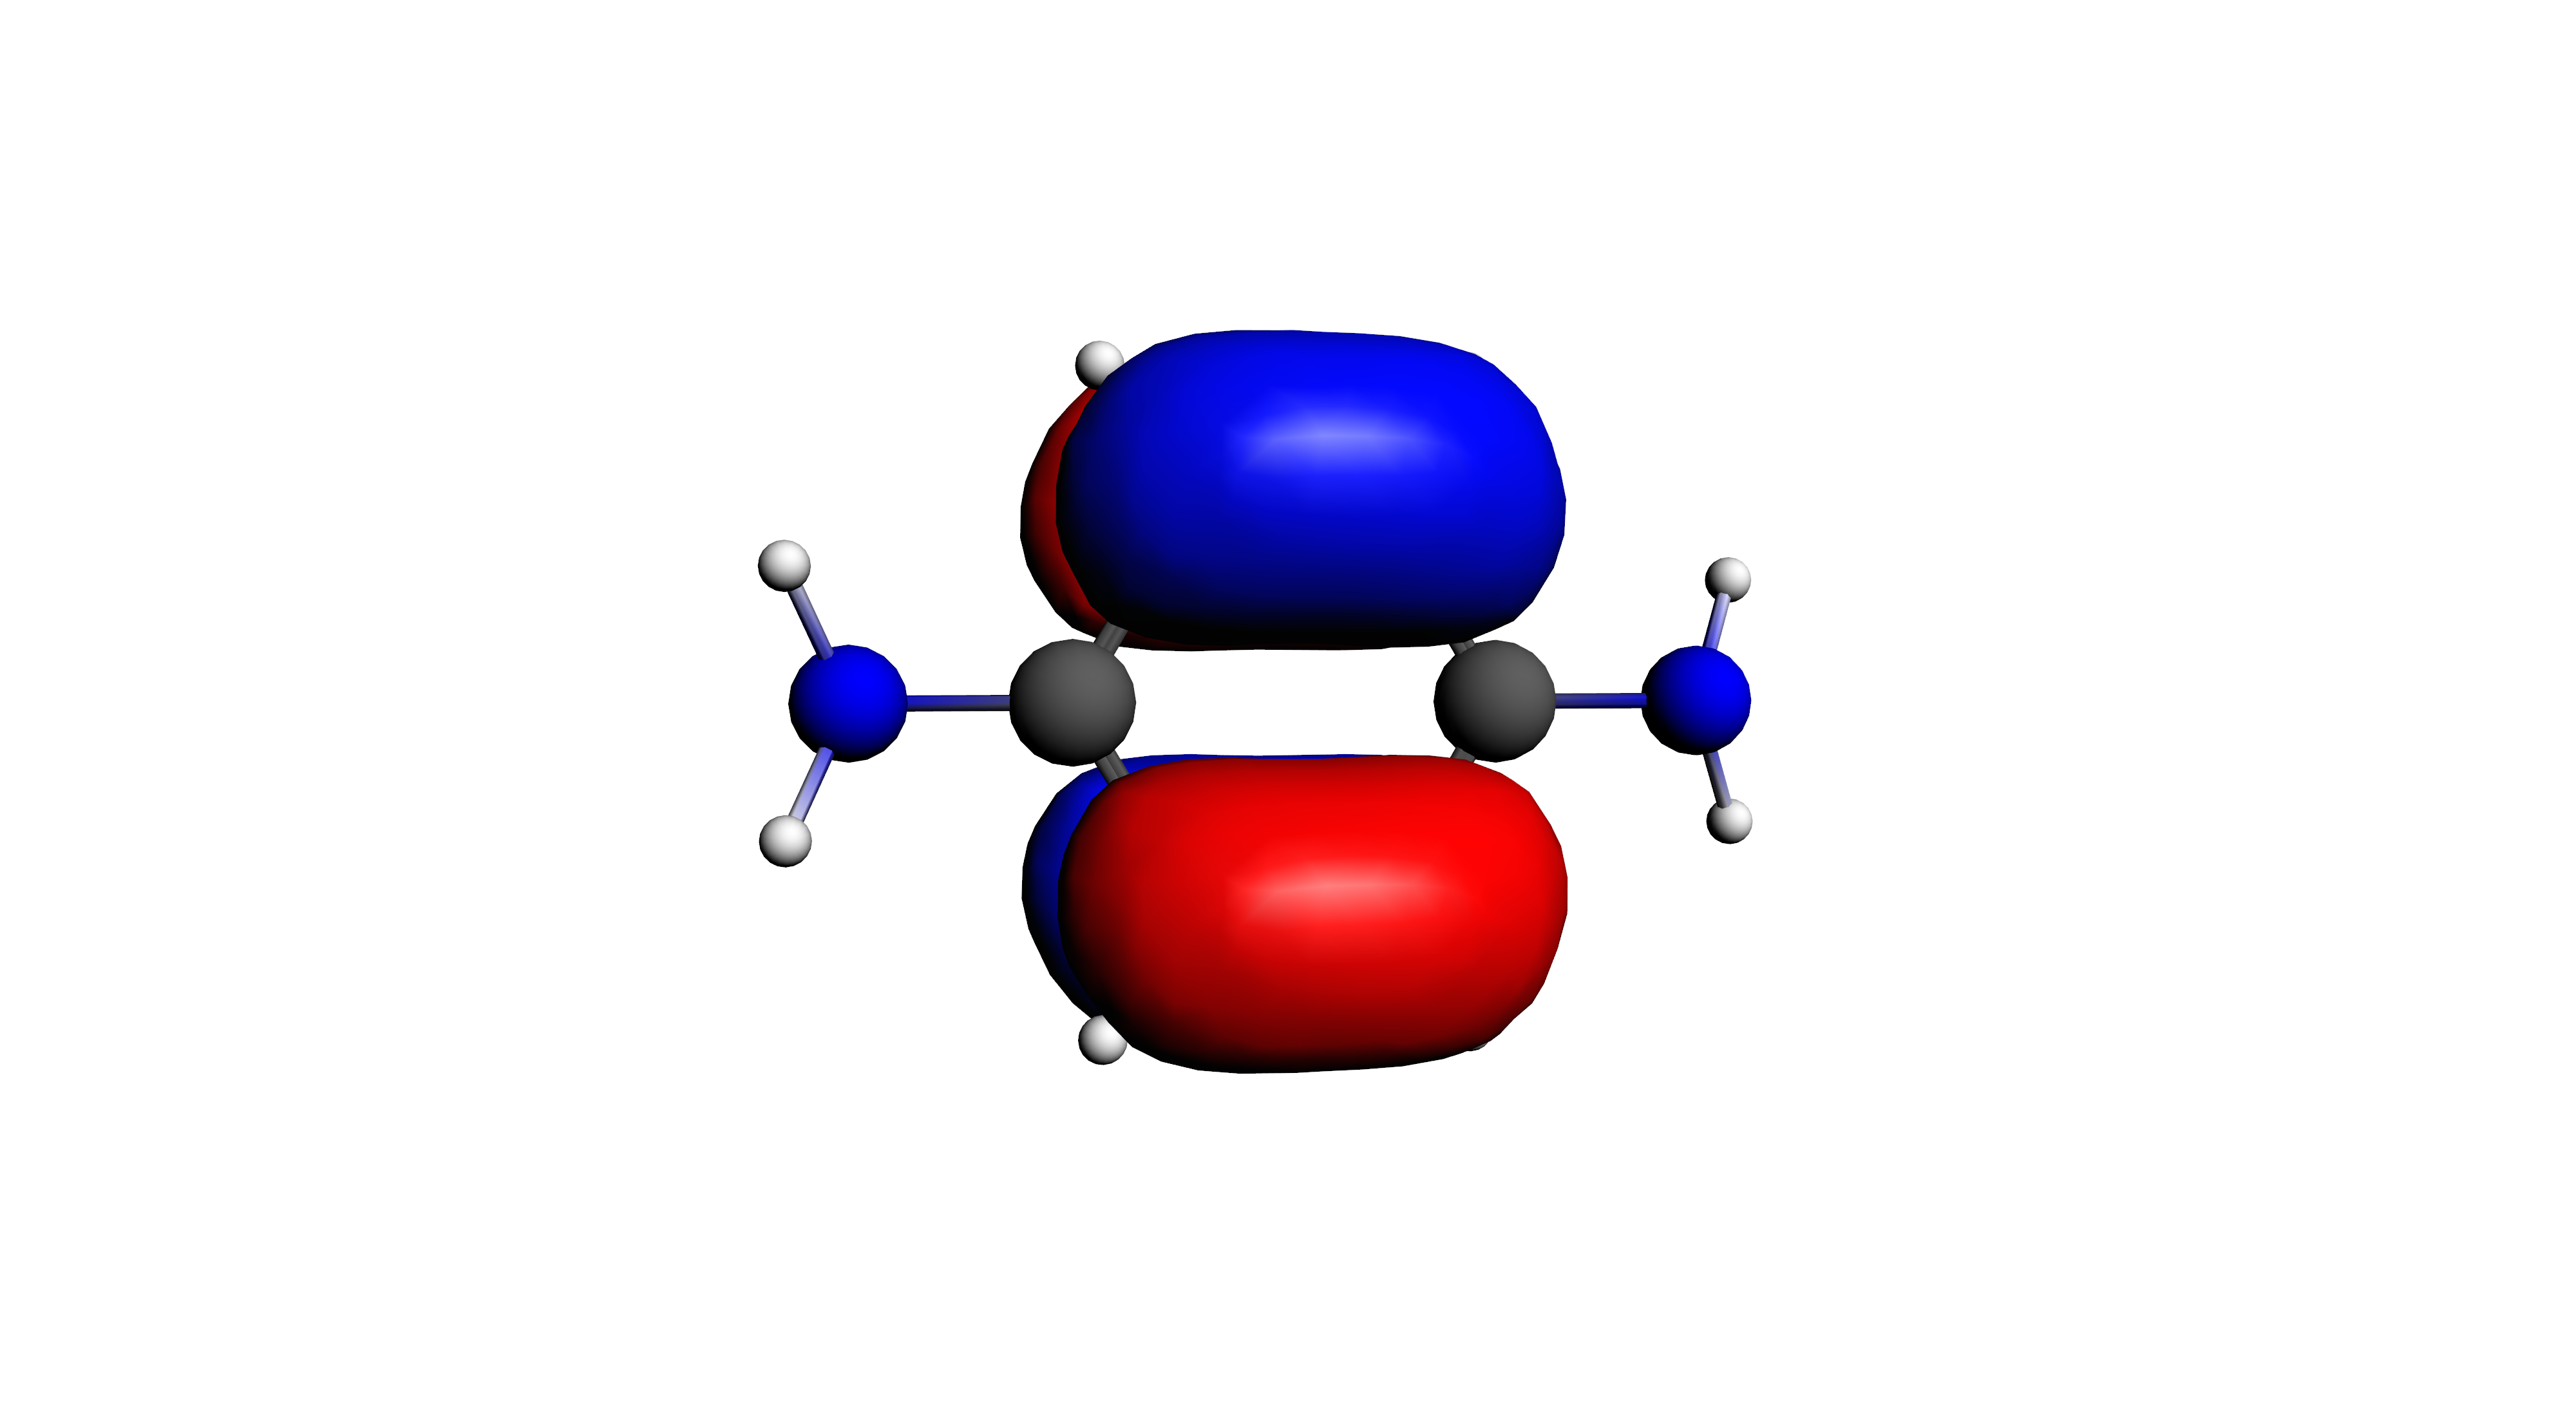
\includegraphics[width=.5\columnwidth]{img.exp/BDA-Levels/gas-phase/HOMO-1.png} }
\caption{Orbitals of BDA molecule in gas-phase ordered by decreasing energy.}\label{fg:BDA-gas}
\end{figure}

\begin{figure}
\subfloat[LUMO+1]{ 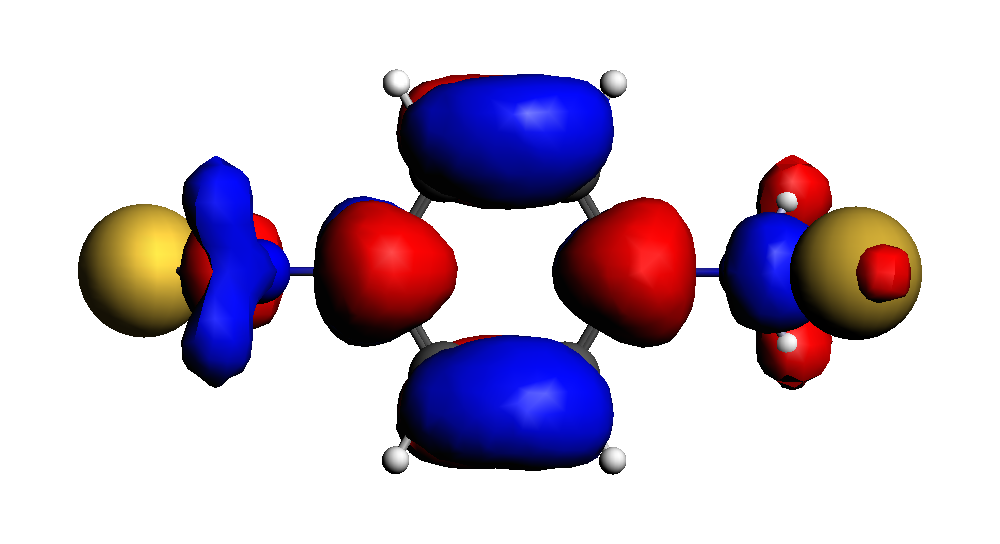
\includegraphics[width=.4\columnwidth]{img.exp/BDA-Levels/fragment/LUMO+1.png} }
\subfloat[LUMO]{ 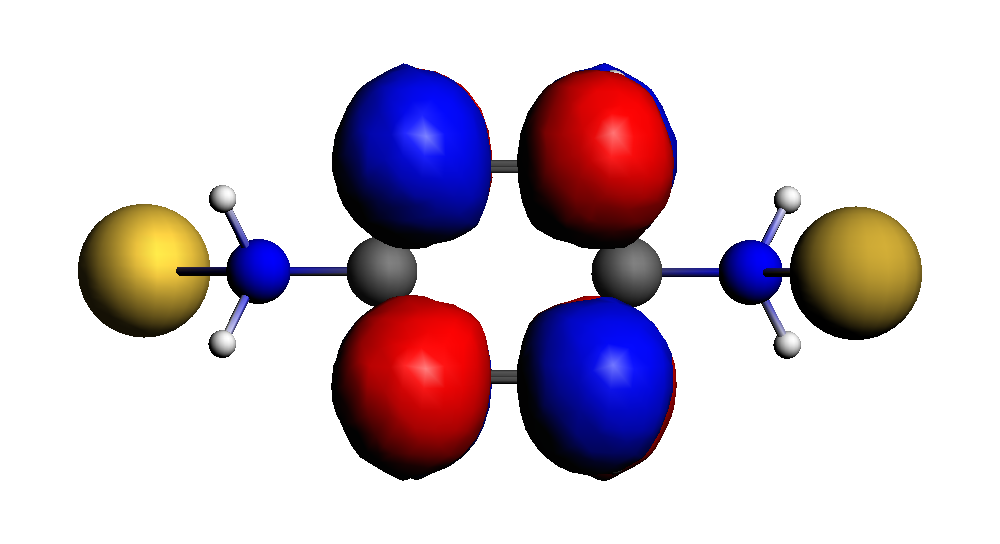
\includegraphics[width=.4\columnwidth]{img.exp/BDA-Levels/fragment/LUMO.png} \label{fg:BDA-frag-LUMO}}\\
\subfloat[Interface state A]{ 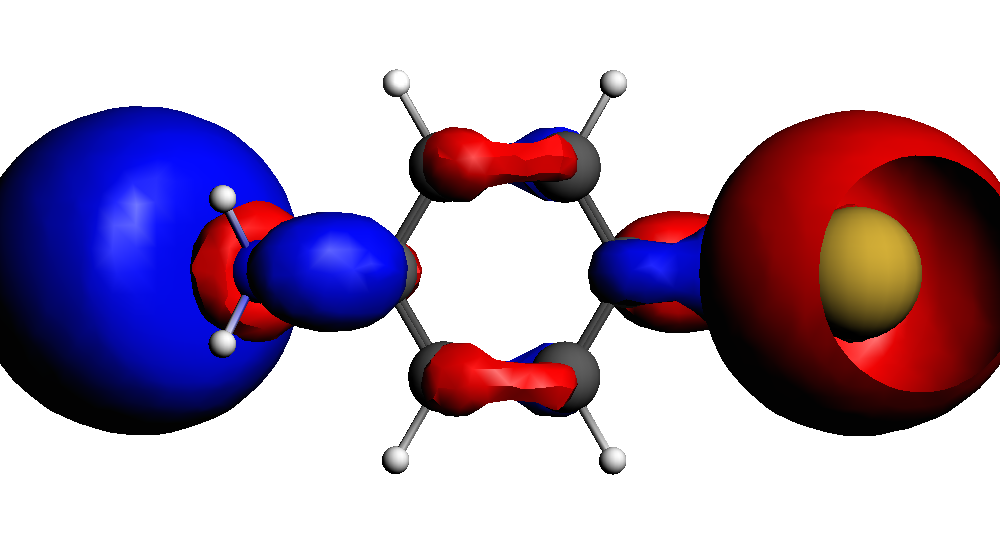
\includegraphics[width=.4\columnwidth]{img.exp/BDA-Levels/fragment/hybrid1.png}\label{fg:BDA-frag-gapA} }
\subfloat[Interface state B]{ 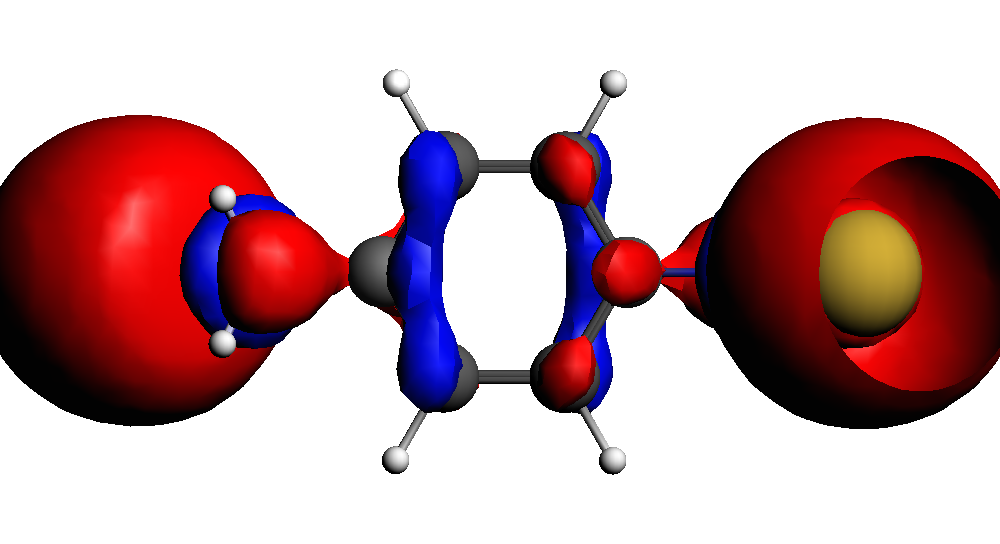
\includegraphics[width=.4\columnwidth]{img.exp/BDA-Levels/fragment/hybrid2.png}\label{fg:BDA-frag-gapB} }\\
\subfloat[HOMO]{ 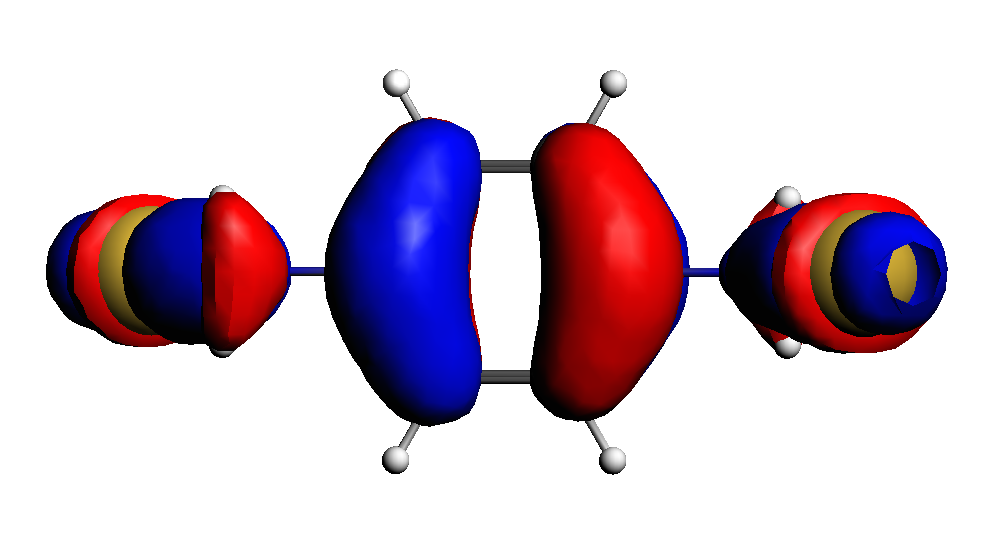
\includegraphics[width=.4\columnwidth]{img.exp/BDA-Levels/fragment/HOMO.png} \label{fg:BDA-frag-HOMO}}
\subfloat[HOMO-1]{ 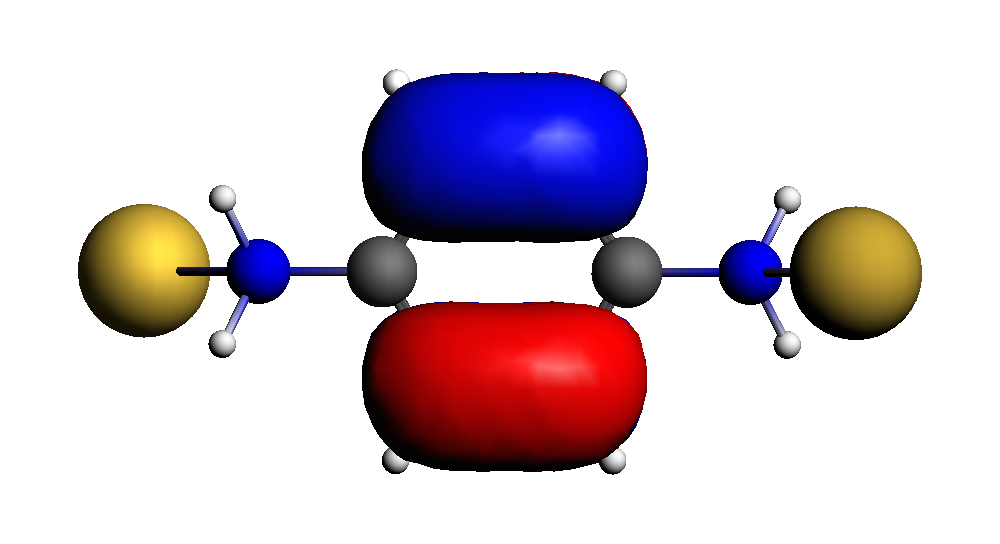
\includegraphics[width=.4\columnwidth]{img.exp/BDA-Levels/fragment/HOMO-1.png} }
\caption{Orbitals of Au-BDA-Au Fragment ordered by decreasing energy.}\label{fg:BDA-frag}
\end{figure}

The main fragment orbitals are labeled by their correspondence with the %BDA 
gas phase orbitals (\eg HOMO Fig. \ref{fg:BDA-frag-HOMO}, LUMO Fig. \ref{fg:BDA-frag-LUMO}, \textit{etc}). There are also intermediate orbitals (Fig. \ref{fg:BDA-frag-gapA} and Fig. \ref{fg:BDA-frag-gapB}), labeled as interface states, which have energies in the HOMO-LUMO gap and are present in the fragment but do not have an analog in the gas phase. The charge density of the interface states has strong contributions on the gold atoms. On the molecule, these states have the structure of the LUMO+1 (Interface state A) and HOMO (Interface state B).


%\subsection{Transport through BDA} \label{Sec:TransportBDA}

To analyze the transport through the molecule, we perform DFT-NEGF calculations for the Au-BDA-Au fragment attached to a FCC (111) surface. We consider a junction of type (I,I) according to the Quek \etal classification \cite{Quek2007} shown in Fig.~\ref{BDA-binding}. For our calculations we use a TZP-basis of numerical atomic orbitals on the molecule, a DZ-basis of numerical atomic orbitals on the metal atoms and the GGA PBE functional in our implementation of NEGF-based transport in the ADF/Band quantum chemistry package \cite{Velde1991,Wiesenekker1991,Verzijl2012}. Computational details can be found in Appendix \ref{computational_methods}. In Appendix \ref{LDA-vs-GGA} we compare the results obtained %for BDA 
using the LDA and GGA functional.

The \textit{reference} charge state of the molecule in the junction is calculated without any bias or gate field applied (see Appendix \ref{LDA-vs-GGA}). The net charge of the molecule is equal to $+0.268e$ with approximately $+0.095e$ on the amines and $+0.173e$ on the rest of the molecule. In this state, the molecule has already some extra charge due to partial charge transfer across the interface \cite{Thygesen2009} (see Fig.~\ref{fg:gated_charges_BDA}). We obtain the charge distributions for the reduced and the oxidized states by gating the levels near to $\epsilon_f$ changing the charge on the molecule by $\approx \pm e$.

%Fig. \ref{fg:gated_charges_BDA} shows the (Hirshfeld) projected charges of the whole molecule, the amine and the molecule excluding the amine.

\begin{figure}
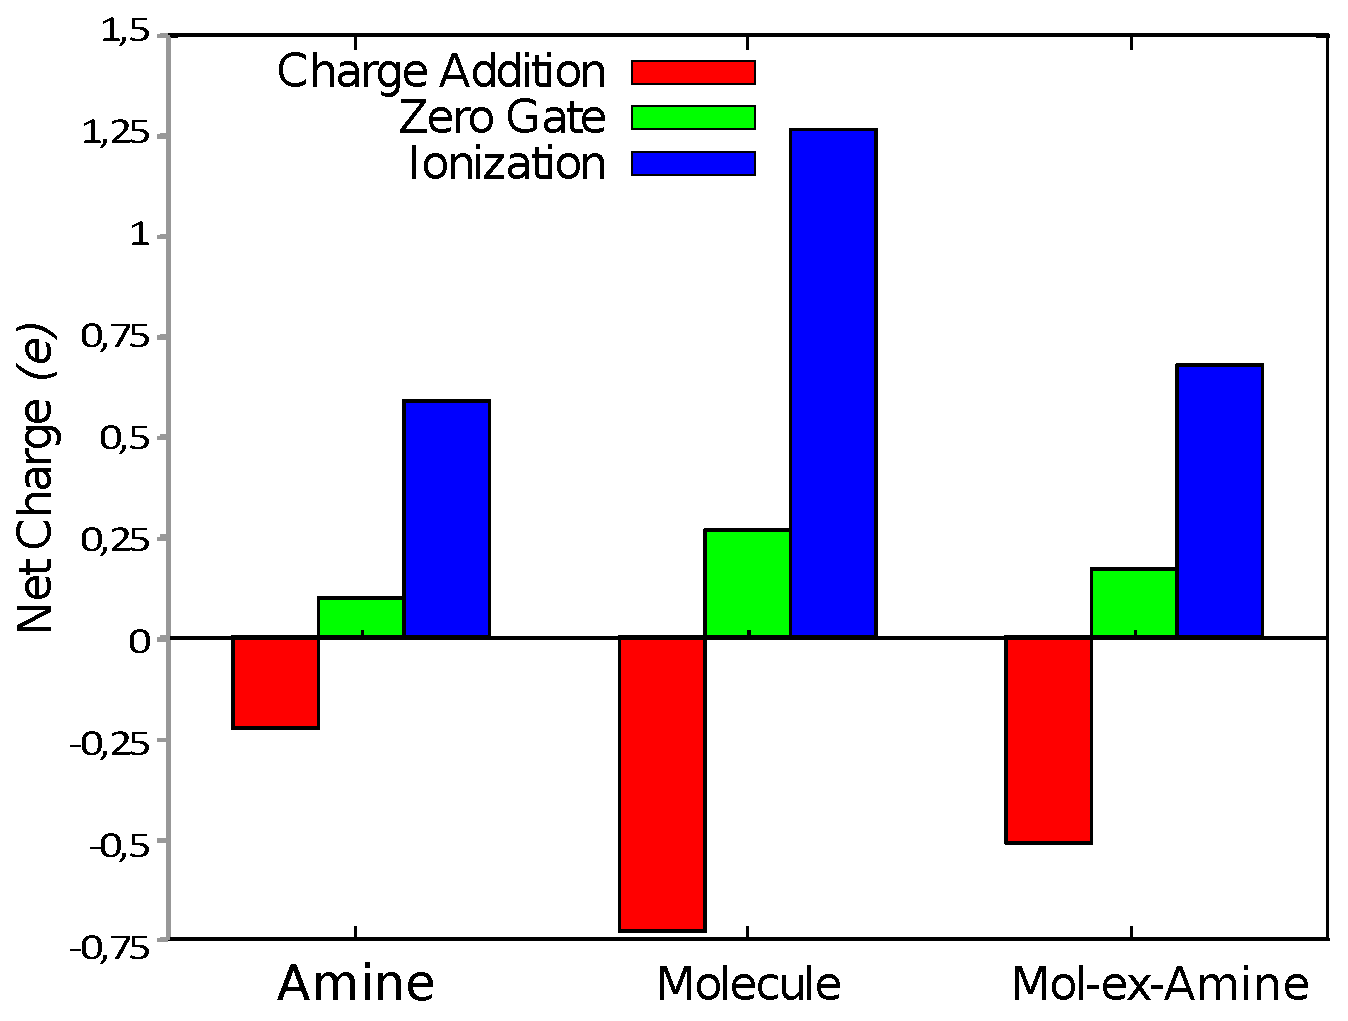
\includegraphics[width=.8\columnwidth]{img/gating-BDA-GGA-N}
\caption{Hirshfeld projected charges for the three gated transport levels (the reference state and $\approx\pm e$ charged states), showing the difference in charging the molecule, amine groups and molecule-without-amine as the gate field is varied.} \label{fg:gated_charges_BDA}
\end{figure}

Fig.~\ref{fg:BDA-peak-composition} shows the compositions of the peaks in the transmission through the Au-BDA-Au junction near $\epsilon_{f}$. For these, we project the eigenstates of the transport calculation onto the orbitals of the Au-BDA-Au fragment \cite{Verzijl2012}.

%From the orbitals in Fig.~\ref{fg:BDA-frag},  we construct Fig.~\ref{fg:BDA-peak-composition} where we show the compositions of the peaks in the transmission through the Au-BDA-Au junction near $\epsilon_{f}$. For these, we use a fragment-decomposition technique, in which we project the eigenstates of the transport calculation onto the orbitals of the Au-BDA-Au fragment \cite{Verzijl2012}.

%As expected, the HOMO-resonance corresponds to the HOMO orbital of the  Au-BDA-Au fragment orbital.
The HOMO projection is distributed in many energies as a result of the hybridization with Au, in contrast to the LUMO, the LUMO$+1$ and the HOMO$-1$ states. The HOMO and LUMO$+1$ are more dominant in charge transport than the LUMO and HOMO$-1$ states which contribute weakly due to their strong localization at the center of the molecule. The interface states ${A}$ and ${B}$ do not show up as peaks in the transmission. We can explain this because these two orbitals have very low density at the center of the molecule as we can see in Fig. \ref{fg:BDA-frag-gapA} and Fig \ref{fg:BDA-frag-gapB}. %This suggest that the transport through BDA is mainly due to the HOMO and LUMO+1. 

\begin{figure}
   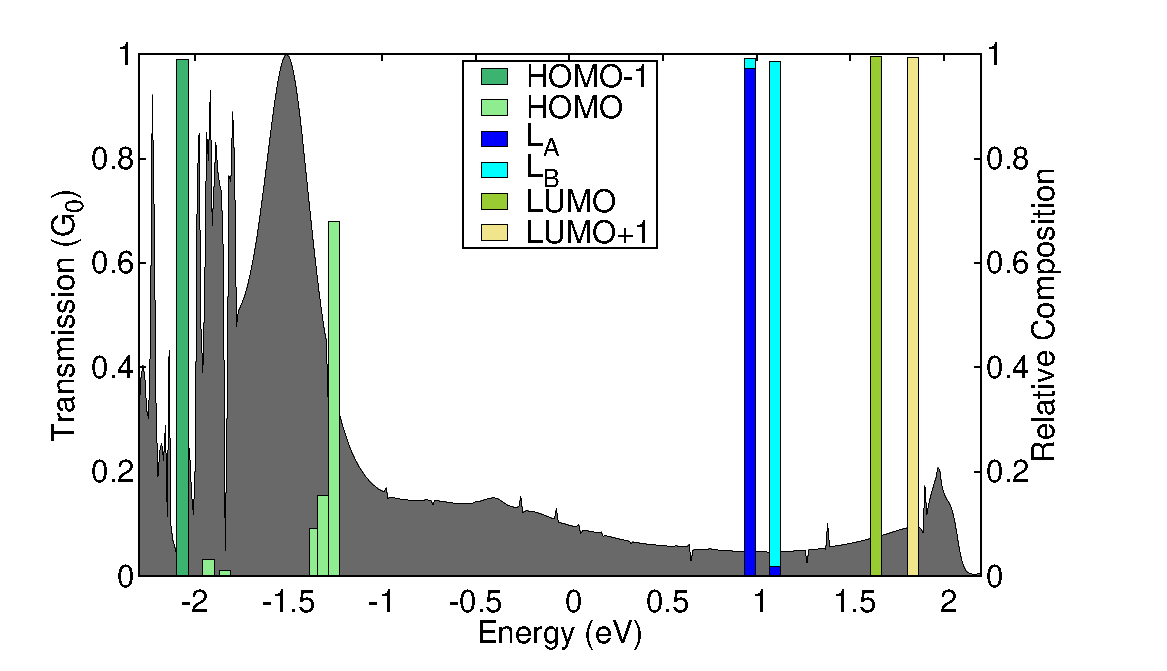
\includegraphics[width=\columnwidth]{img/BDA/BDA-decomposition}
\caption{Peaks Decomposition with fragment Orbital Levels (grey shaded curve is transmission). Composition of peaks in transport, constructed by projection onto fragment molecular orbitals. A state with value 1 is a decoupled state, and completely un-hybridized (\eg HOMO-1), while HOMO, is strongly hybridized, with the rest originating from Au).}\label{fg:BDA-peak-composition}
\end{figure}



\subsection{Image-Model Calculations on BDA}\label{imagemodelcalcsBDA}

%Mowbray's model uses the molecule in gas phase for the calculation of the energy shifts. Additionally, they assume that in the reference state each atom of the molecule has zero charge. For the atomic charge differences with respect to the reference state of the unoccupied orbital they take the opposite of the atomic charge differences of the occupied orbitals.
%Different from Mowbray's \etal calculations, in our model, we consider 
%For the molecule in the junction, %We take the reference state at zero bias and gate. 
%in the reference state, the molecule %in the junction 
%The charge distributions for the reduced and the oxidized states are obtained by gating the levels near to $\epsilon_f$ changing the charge on the molecule by $\approx \pm e$.
For the Image charges calculation, we consider the reduced and the oxidized orbitals separately, which is reflected in a marked difference between shifts for occupied and unoccupied orbitals.

\begin{figure}
\subfloat[Geometry for Image-Charge Shifts]
{
   \raisebox{.6cm}{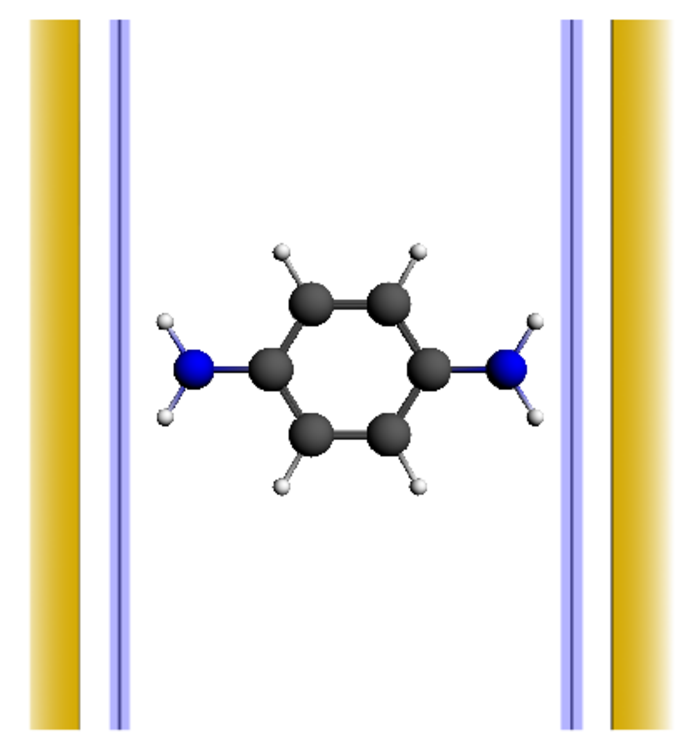
\includegraphics[width=.45\columnwidth]{img.exp/contacts}\label{fg:shiftsgeomBDA}}
}
\subfloat[Transport Gap Renormalization]{
   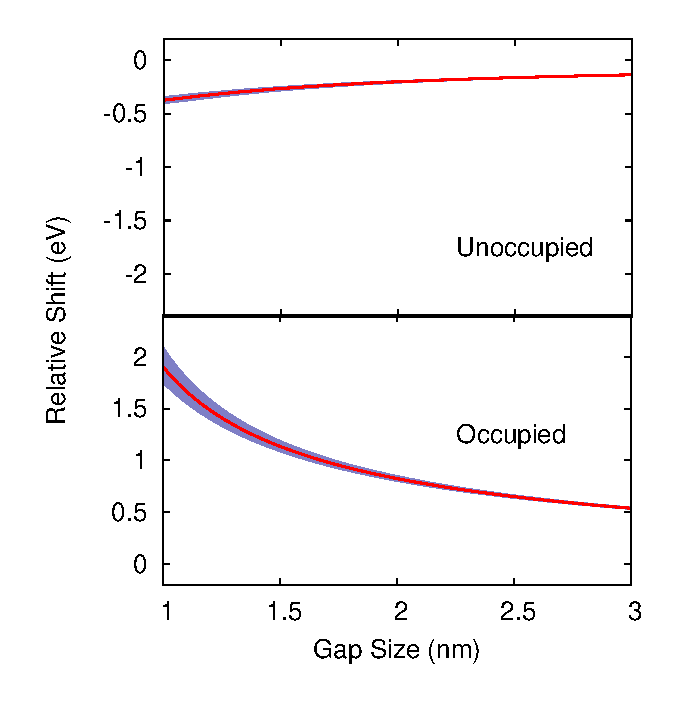
\includegraphics[width=.55\columnwidth]{img/SingleGapPlotBDA}\label{fg:shiftscalcBDA}
}
\caption{(a) Geometry used in the image-charge model (with uncertainties) (b) shifting  to  the occupied and unoccupied levels predicted by the our model as function of the distance between the contacts.
}\label{fg:contactsBDA}
\end{figure}

In Fig.~\ref{fg:shiftsgeomBDA} we show the geometry used for our image-charge model and in Fig.~\ref{fg:shiftscalcBDA} we show the resulting shifts of the occupied and unoccupied levels as function of the distance between the two contacts. The uncertainty bands are calculated based on a $\pm0.25\ \AA$ uncertainty in the position of the image planes.

In Fig.~\ref{fg:gas_vs_junction_BDA}, we compare the results obtained by our method using different assumptions during the calculations. The dashed line is calculated using the gas phase charge distribution, zero charge on each atom for the reference state and omit the atomic charges associated with the EA, following the Mowbray \etal assumptions. %This curve is in agreement with Mowbray's model. 
Once we include the effects due to the EA (purple line), the symmetry for the shifts of the occupied and unoccupied levels is not maintained. Furthermore, if we use the charge distribution of the neutral molecule as reference state (red line), those differences increase notably. Finally, using the junction charge distribution (green line), we see a clear difference. This shows that by using charges obtained with the junction geometry (from a NEGF+DFT calculation) for the image-charge calculation, we are including features that are absent when the gas phase charges are used.

\begin{figure}
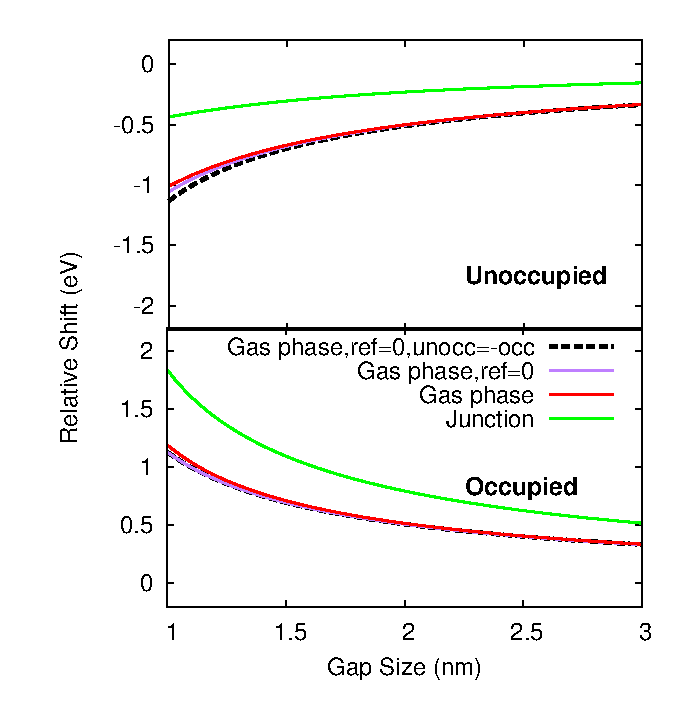
\includegraphics[width=.8\columnwidth]{img/Methods/Us_vs_Mowbraygas_BDA-ref}
\caption{Comparison of results for total image-charge corrections using charges from gas phase calculations of BDA and from the molecular junction.} \label{fg:gas_vs_junction_BDA}
\end{figure}




\section{Au-ZnTPPdT Molecular Devices} \label{Sec:ZnTPP}

We now proceed to a more complicated application of the method, which allows for comparison with a recent experiment that revealed the image-charge effects on both occupied and unoccupied molecular levels.


\subsection{Experimental Results}\label{experiments}

We consider the experimental findings of Perrin \etal\cite{Perrin2011a,Perrin2011b,Perrin2013} who studied thiol-terminated zinc-porphyrin molecules [Zn(5,15-di(p-thiolphenyl)-10,20-di(p-tolyl)porphyrin)], abbreviated as ZnTPPdT. 
In the experiments, the current was recorded as a function of gate and bias voltage, and of the electrode separation.
Peaks in the differential conductance were identified as transport resonances.
These resonances show a marked ``mechanical gating'' effect, where a level shift is induced by a change in the metal-molecule distance (for both the occupied and unoccupied levels of the molecule). The efficiency of the effect can be expressed by a mechanical gate coupling (MGC) defined as 
\begin{equation}
\epsilon_F=\frac{d V_b}{dx}, 
\end{equation}
where $V_b$ is the bias voltage and $x$ the electrode separation . 

We show experimental data for these shifts in Fig.~\ref{fg:experiment}, where the measurements show a distance-dependent energy for the lowest resonance. A linear fit of the resonance positions was used to find the MGC. 
The broadness of the distribution is presumably due to the fact that ZnTPPdT is not a rod-like molecule; it can form molecular junctions with various geometries, as has been reported previously for similar molecules.\cite{Perrin2011b}

\begin{figure}
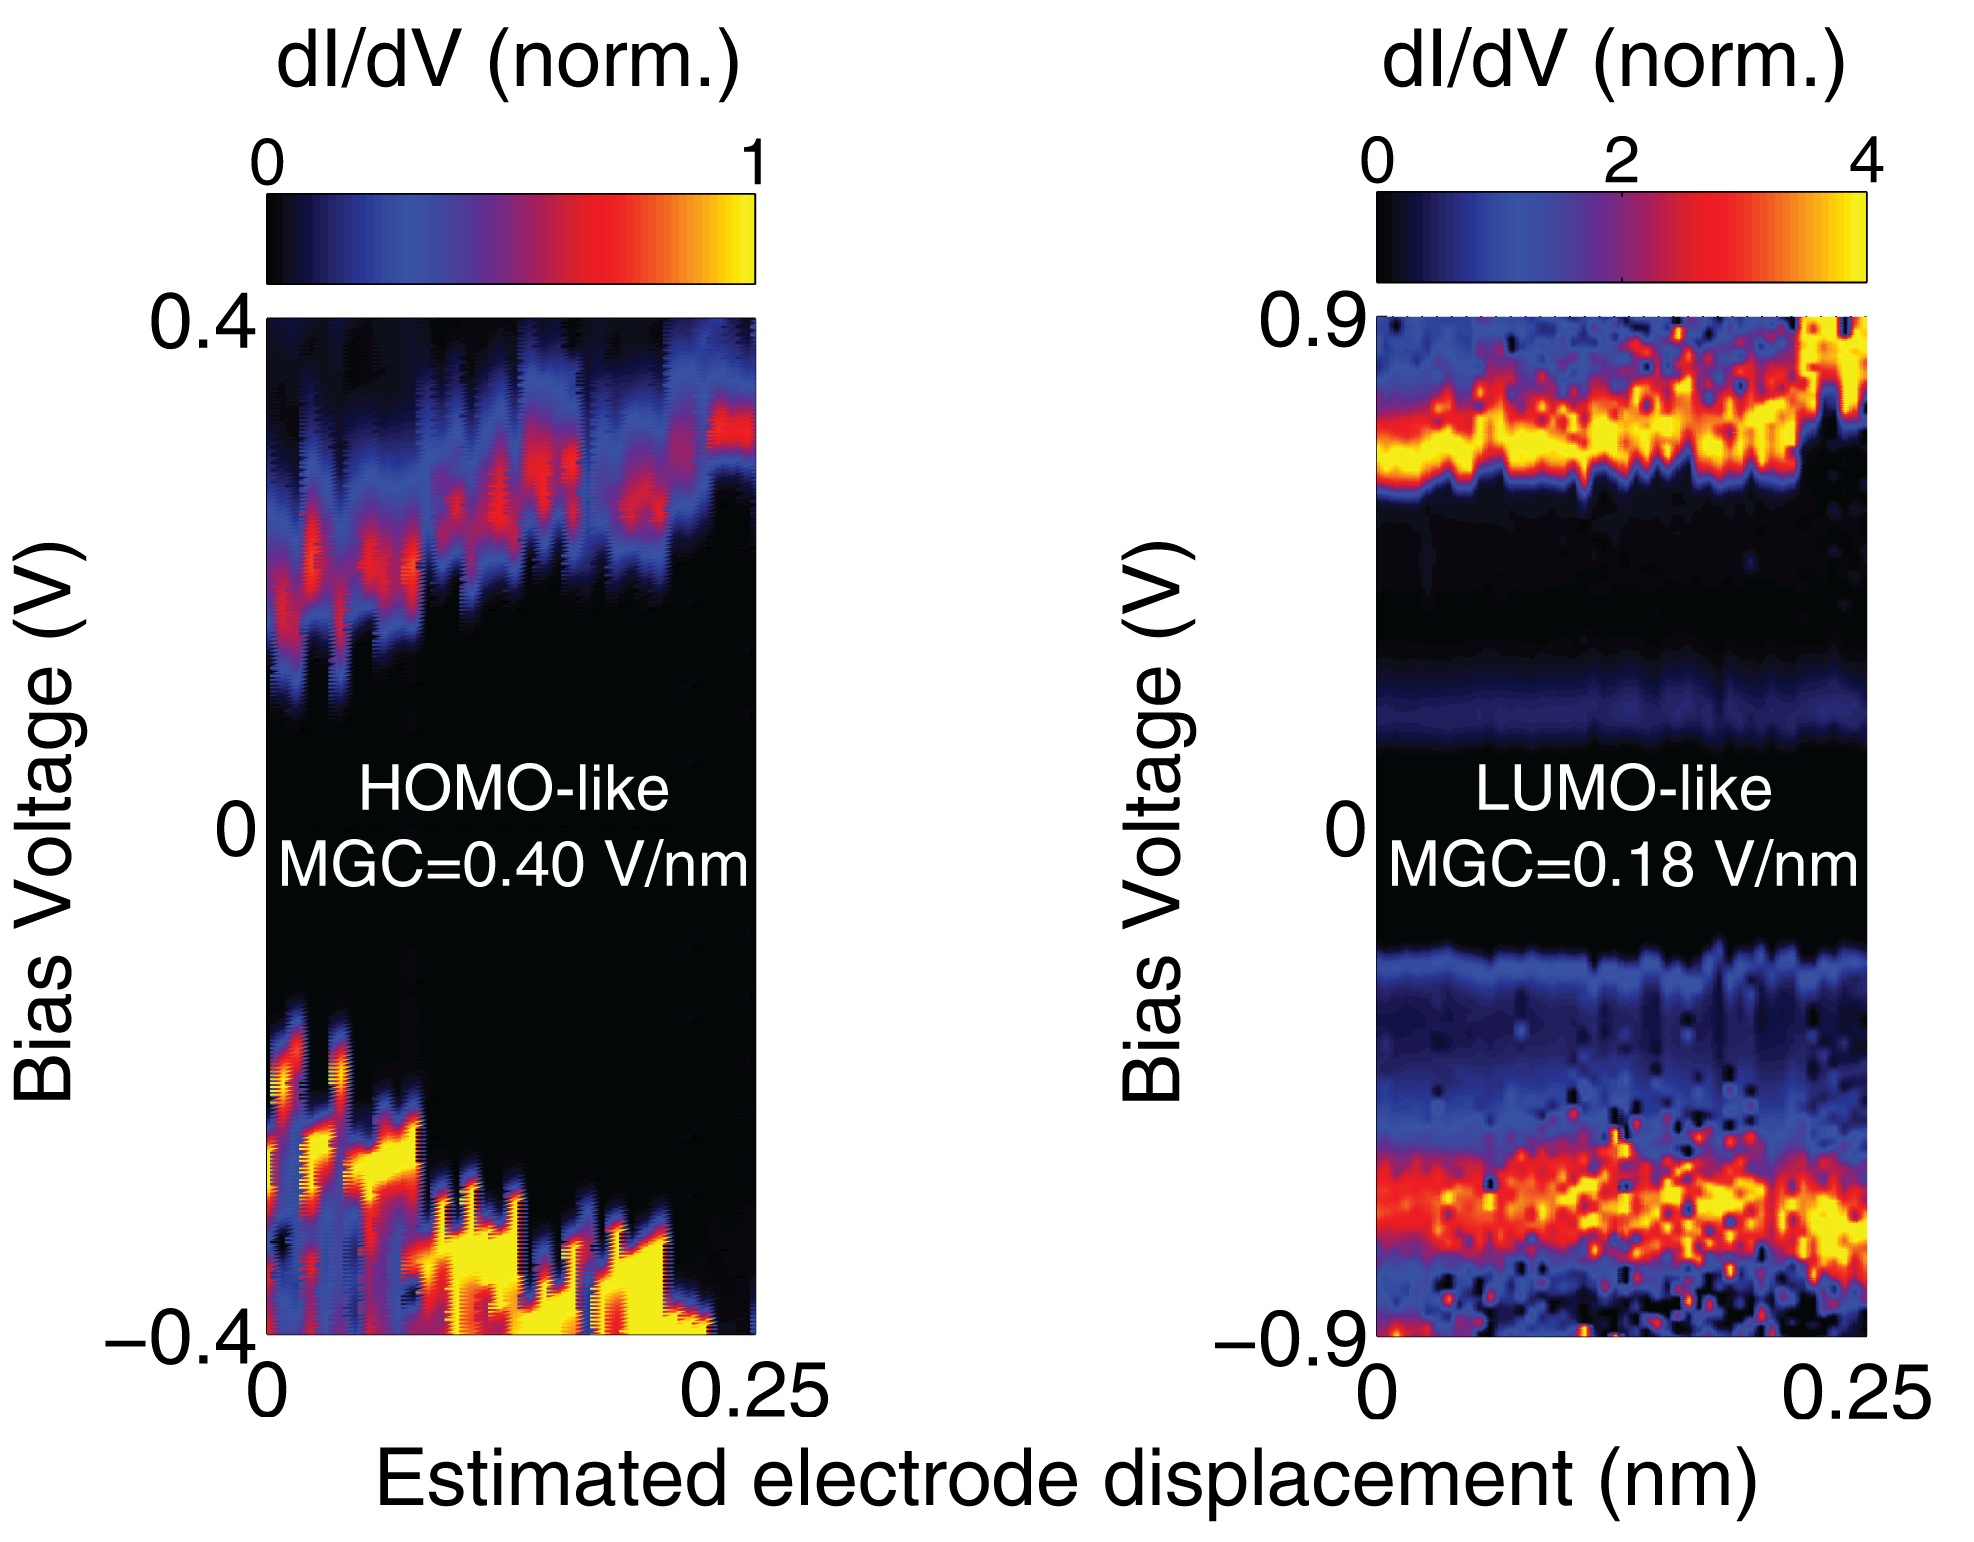
\includegraphics[width=.9\columnwidth]{img/Fig3TH}\label{fg:exp_measurement}

\caption{Representative measurement,\cite{Perrin2013} showing HOMO-like and LUMO-like observed MGC's. Note the dilation of the y-axis in the case of LUMO-like resonances. 
}
\label{fg:experiment}
\end{figure}

The MGC's values are 
in the range of $0.2-1$ $V_b$/nm 
Combined with a typical range of $0.5$ nm over which the junctions formed are stable, 
implying levels shift of roughly $50-250$ meV in energy, if we assume the bias voltage  drops symmetrically. An average MGC values of $0.40$ V/nm was found for occupied, and  $0.18$ V/nm for unoccupied levels.


\subsection{Calculations}\label{calculations}

We will now show that our approach yields trends matching the experiment, and explains the asymmetry in the shifts found between occupied and unoccupied levels. 



% \subsubsection{ZnTPPdT Electronic Structure}\label{electronic_structure}


%\begin{figure}
%\subfloat[ZnTPPdT Gas-Phase Geometry]{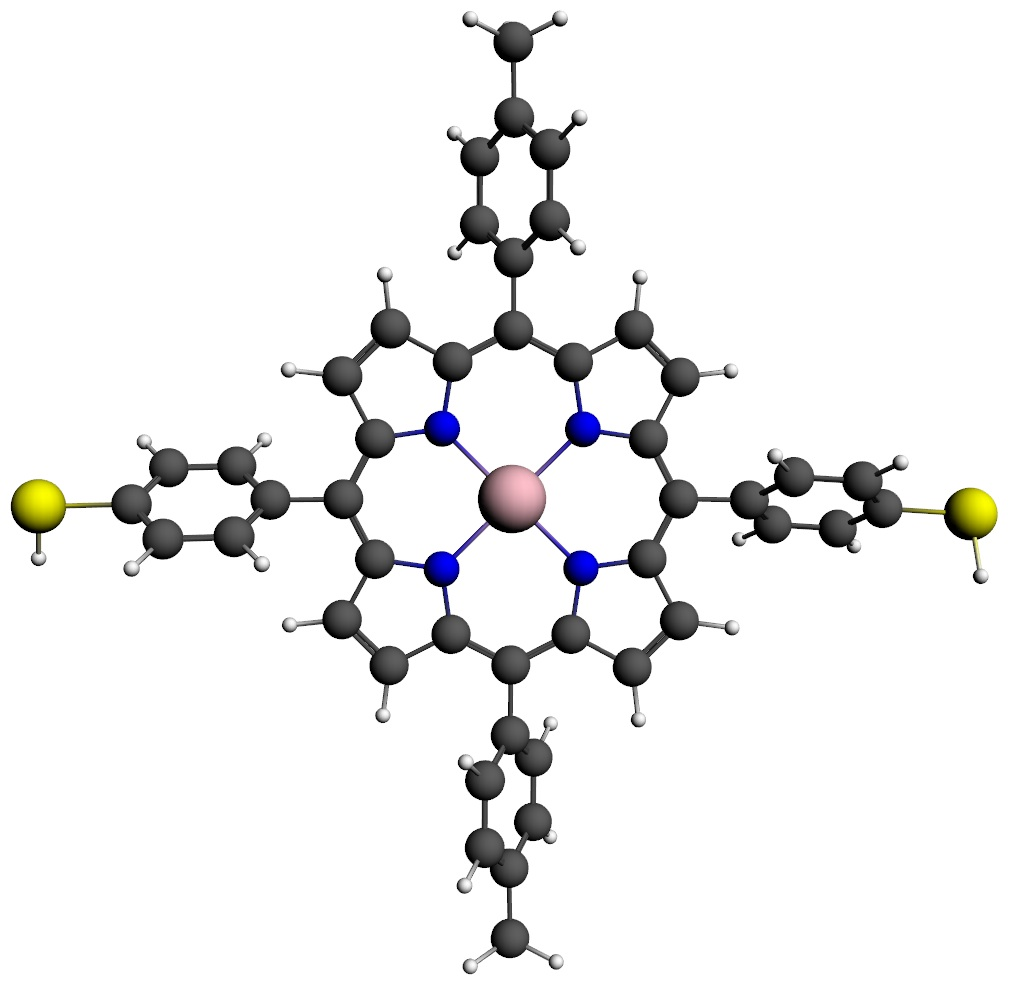
\includegraphics[width=.425\columnwidth]{img.exp/Fragment-geoms/ZnTPP-fragment}}\hfill
%\subfloat[Au-ZnTPPdT Fragment Geometry]{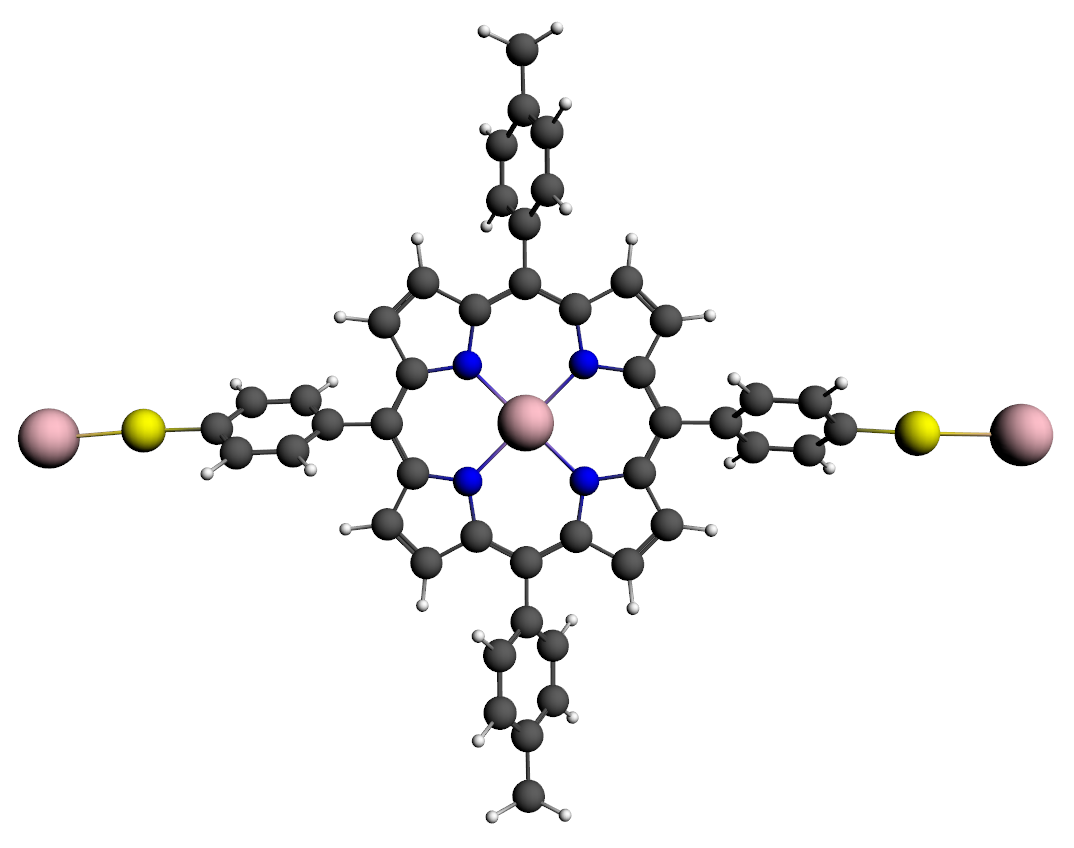
\includegraphics[width=.525\columnwidth]{img.exp/Fragment-geoms/ZnTPP-fragment-au}}\\
%\subfloat[Au-ZnTPPdT Junction Geometry]{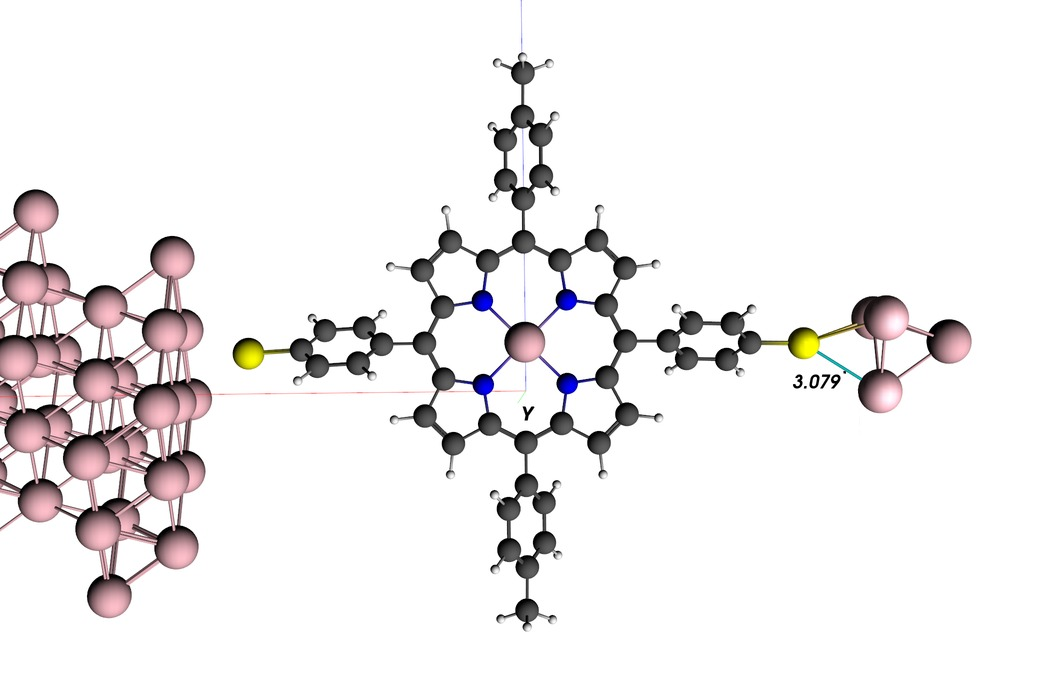
\includegraphics[width=.9\columnwidth]{img.exp/ZnTPP-binding1} \label{ZnTPP-binding}}
%\caption{Geometries of ZnTPPdT in (a) gas phase and (b) as a fragment. Metal ions are pink-grey. (c) Typical binding geometry. Left Au atoms show placement relative to a (111) surface layer, right atoms show the positions of nearest neighbors participating in the hollow-site Au-S binding. In the transport calculations bulk-like contacts are present on both sides.}\label{fg:4geometries}
%\end{figure}


%To apply our method to this molecular junction, we first 
%consider the electronic structure of the molecules in gas phase. 
%Computational details can be found in appendix \ref{computational_methods}. The geometries for gas phase and fragments with gold atoms are illustrated in Fig.~\ref{fg:4geometries} and the resulting electronic structure is shown schematically in Fig.~\ref{fg:ZnTPP-levels} for the three relevant gas phase charge states.


%\begin{figure}
% \fbox{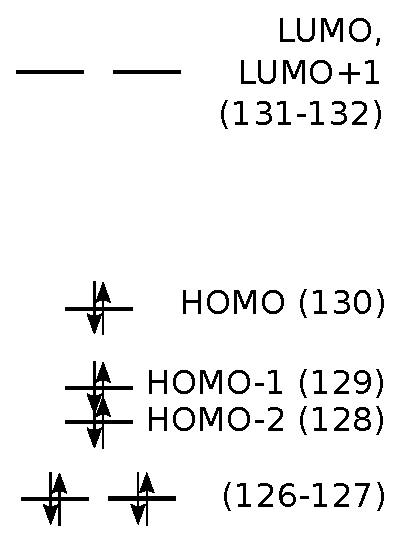
\includegraphics[width=.33\columnwidth]{img.exp/Illustration/n_occups_Zn}}
%\caption{Highest occupied and lowest unoccupied level structure of the ZnTPPdT molecule in gas phase, with $130^\text{th}$ occupied valence orbital corresponding to a total of $260$ valence electrons used in the DFT calculation (with lower lying levels treated in the frozen-core approximation). The corresponding orbitals are illustrated in Figs.~\ref{fg:ZnTPP-frag} and \ref{fg:ZnTPP-gas}.}\label{fg:ZnTPP-levels}
%\end{figure}


\begin{figure}
\subfloat[LUMO+1]{ 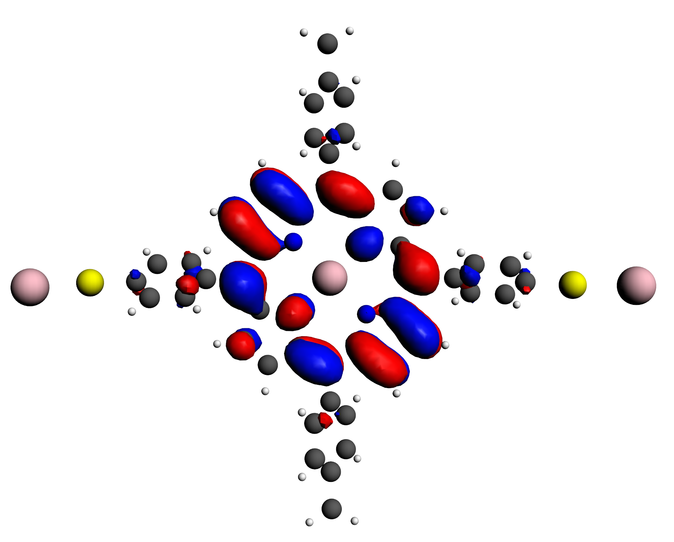
\includegraphics[width=.35\columnwidth]{img.exp/ZnTPP-Levels/fragment/LUMO+1.png} }
\subfloat[LUMO]{ 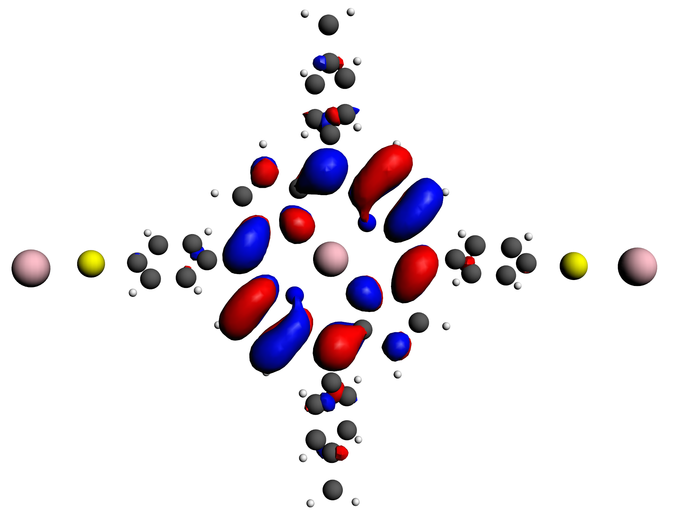
\includegraphics[width=.35\columnwidth]{img.exp/ZnTPP-Levels/fragment/LUMO.png} }\\
\subfloat[Interface State A]{ 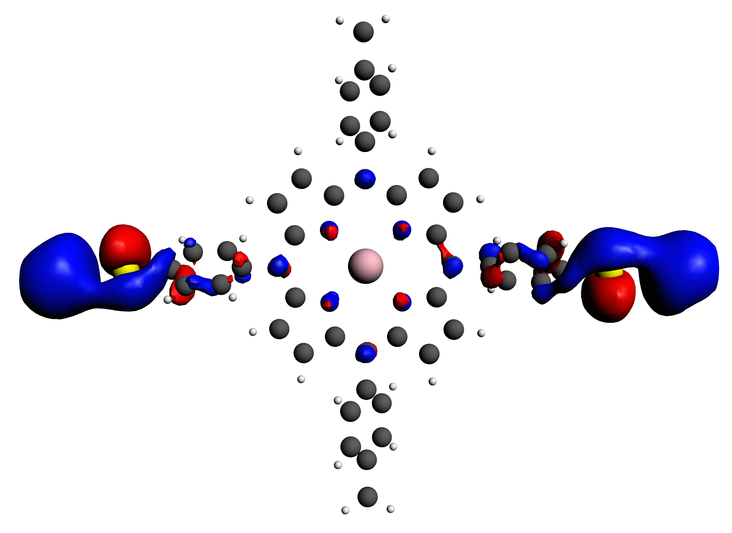
\includegraphics[width=.35\columnwidth]{img.exp/ZnTPP-Levels/fragment/gap1C.png} }
\subfloat[Interface State B]{ 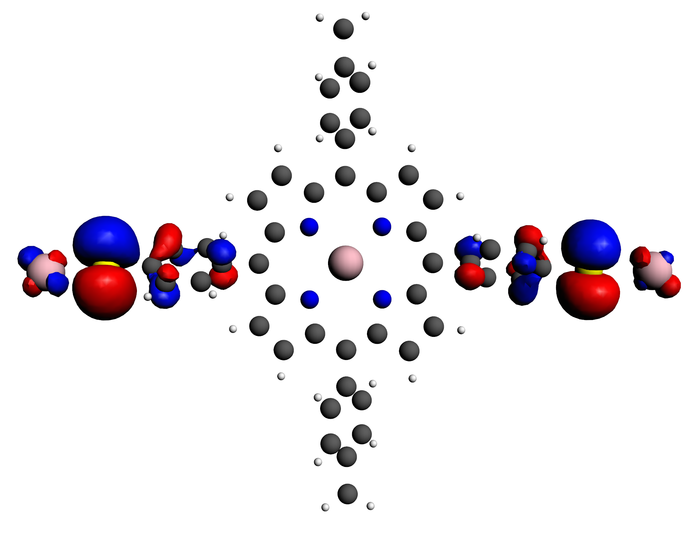
\includegraphics[width=.35\columnwidth]{img.exp/ZnTPP-Levels/fragment/gap2A.png} }\\
\subfloat[HOMO]{ 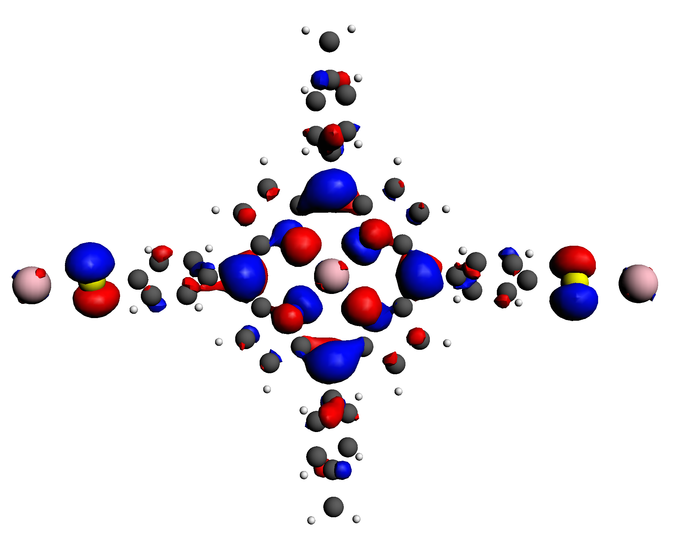
\includegraphics[width=.35\columnwidth]{img.exp/ZnTPP-Levels/fragment/HOMO.png} }\\
\subfloat[HOMO-1]{ 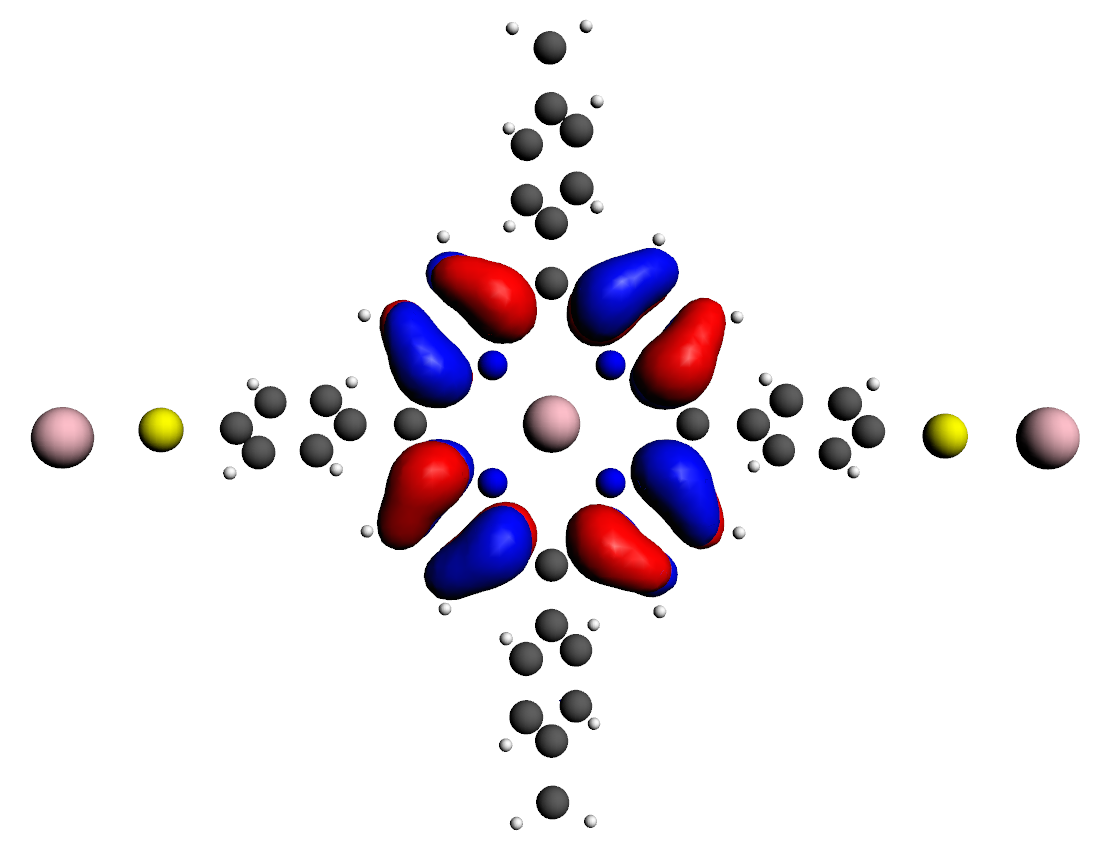
\includegraphics[width=.35\columnwidth]{img.exp/ZnTPP-Levels/fragment/fragment-HOMO-1.png} }
\subfloat[HOMO-2]{ 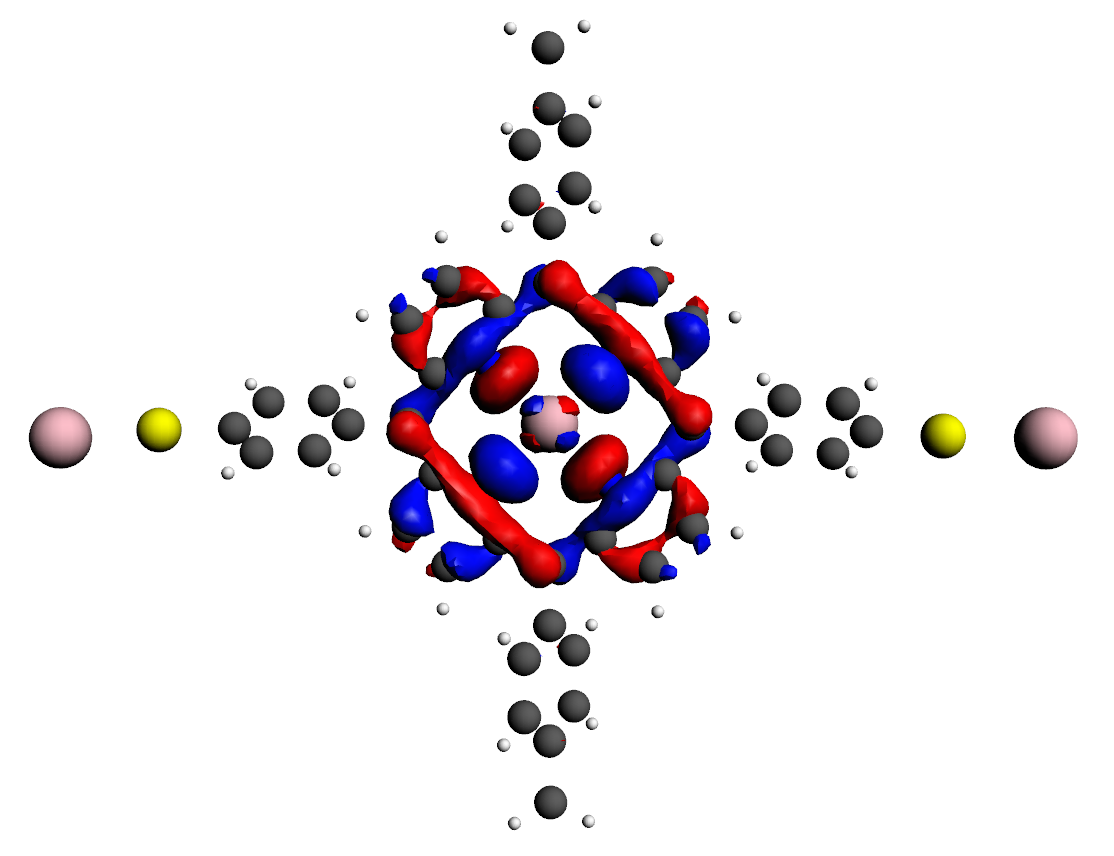
\includegraphics[width=.35\columnwidth]{img.exp/ZnTPP-Levels/fragment/fragment-HOMO-2.png} }
\caption{Orbitals of gas phase Au-ZnTPPdT-Au Fragment. (c)-(d) Typical interface levels which form on hybridizing with Au: 6 total between the analogue of the gas phase HOMO and LUMO (see Fig.~\ref{fg:ZnTPP-gas}), forming three sets of bonding/anti-bonding pairs, of which two sets with HOMO character and one set with LUMO character.}\label{fg:ZnTPP-frag}
\end{figure}

We focus on the frontier orbitals (HOMO and LUMO) which are generally considered to be the most useful for transport. We find a the HOMO-LUMO gap to be $1.8$ eV in our LDA and GGA calculations and $2.7$ eV using the B3LYP functional, consistent with the reports of Park \etal\cite{Park2008}, and in general agreement with their redox measurements of roughly $2.2$ eV. %This value suggests that it would be impossible to observe both HOMO and LUMO resonances in the experiment where the bias range is limited to about $1.0$ V.

In figure~\ref{fg:ZnTPP-frag}, we show the orbitals of the ZnTTP-fragment, which contains two extra gold atoms. We see direct counterparts of the LUMO, HOMO and HOMO-1 of the gas phase (which have given the same name in figure~\ref{fg:ZnTPP-frag}), but also new orbitals which have a substantial contibution 
on the arms of the molecule binding to the gold -- we call those \emph{interface states}. The orbital levels in the fragment appear to be of a 
bonding/anti-bonding character, with splittings on the order of $0.1$ eV.CHRIS: other IF states?????

%The relevant molecular levels for transport in Fig.~\ref{fg:ZnTPP-levels} are those which are near the Fermi level of the Au electrodes. We show the levels HOMO$-2$ through LUMO$+1$ for the fragment in Figs.~\ref{fg:ZnTPP-frag} (see Fig.~\ref{fg:ZnTPP-gas} for the orbitals of the gas phase). Most levels are characterized by an orbital wave-function which extends at least somewhat onto the arms connecting the molecule to the electrodes, and the coupling from the arms to the electrodes almost fully determines the relevance of the orbital for transport. The HOMO-like levels extend more onto the arms than the LUMO, and the fragment orbitals in Fig.~\ref{fg:ZnTPP-frag} suggest that they also hybridize more strongly with the gold.

%Most of the fragment orbitals can be directly related to gas phase orbitals by considering their symmetry on the molecule. For a  number of levels, this connection is less straightforward, these are interface states (see Fig.~\ref{peak-compositions}).  
%Their charge density is located mostly on the arms, and they appear to be stabilized by the interface.  

%We find  the HOMO-LUMO gap to be $1.8$ eV in our LDA and GGA calculations and $2.7$ eV using the B3LYP functional, consistent with the reports of Park \etal\cite{Park2008}, and in general agreement with their redox measurements of roughly $2.2$ eV. This value suggests that it would be impossible to observe both HOMO and LUMO resonances in the experiment where the bias range is limited to about $1.0$ V.







%\subsubsection{Transport through ZnTPPdT Junctions}\label{transport}


Our Au-ZnTPPdT binding geometry is based on a phenyl ring bonded to an FCC (111) gold surface via a thiolate bond, in a hollow-site configuration.\cite{Nara2004,Andrews2006,Kondo2006,Pontes2011}
% as shown in Fig.~\ref{ZnTPP-binding}. 
In the calculations, the binding is characterized by chemisorption, with significant charge transfer to the thiols, which act as acceptors. This is in agreement with the literature on such bindings.\cite{Xue2003a,Xue2003b,Love2005,Hoft2006,Romaner2006} %The calculations are performed with a perpendicular hollow-site binding to a FCC (111) surface. 


All calculations were performed using a TZP-basis of numerical atomic orbitals on the molecule, using the LDA functional  with thiols located at a 2.59\AA\xspace from the electrodes. For further details concerning the calculations, see appendix \ref{computational_methods}.\\

\begin{figure}
\subfloat[Peaks Decomposition with Molecular Orbital Levels (grey shaded curve is transmission)]{
   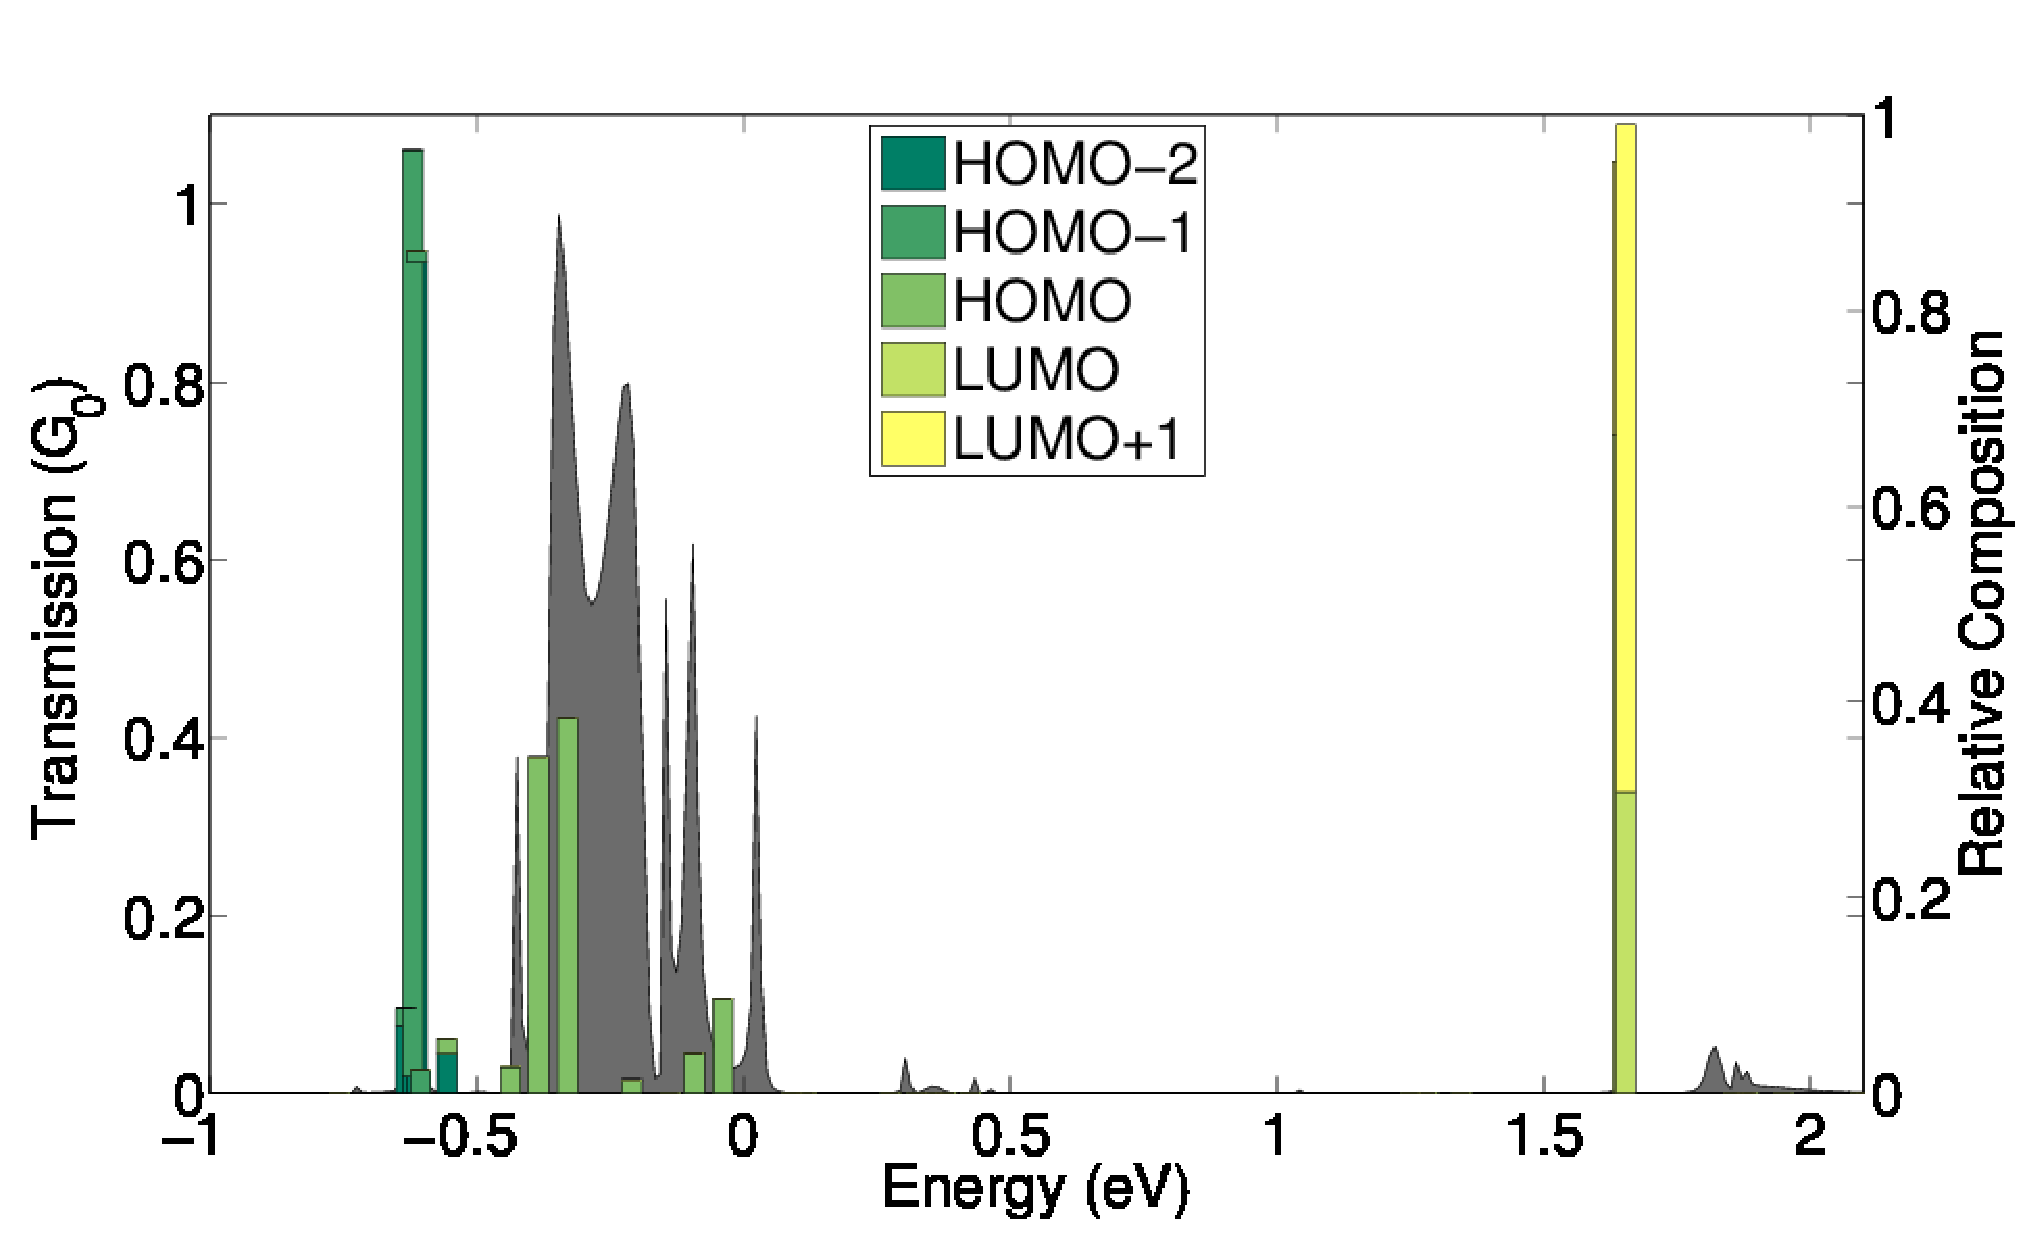
\includegraphics[width=\columnwidth]{img/ZnTPPdT/ZnTPP_peaks}\label{fg:decompositions}
   }\\
\subfloat[Peaks Decomposition with Interface Levels]{
   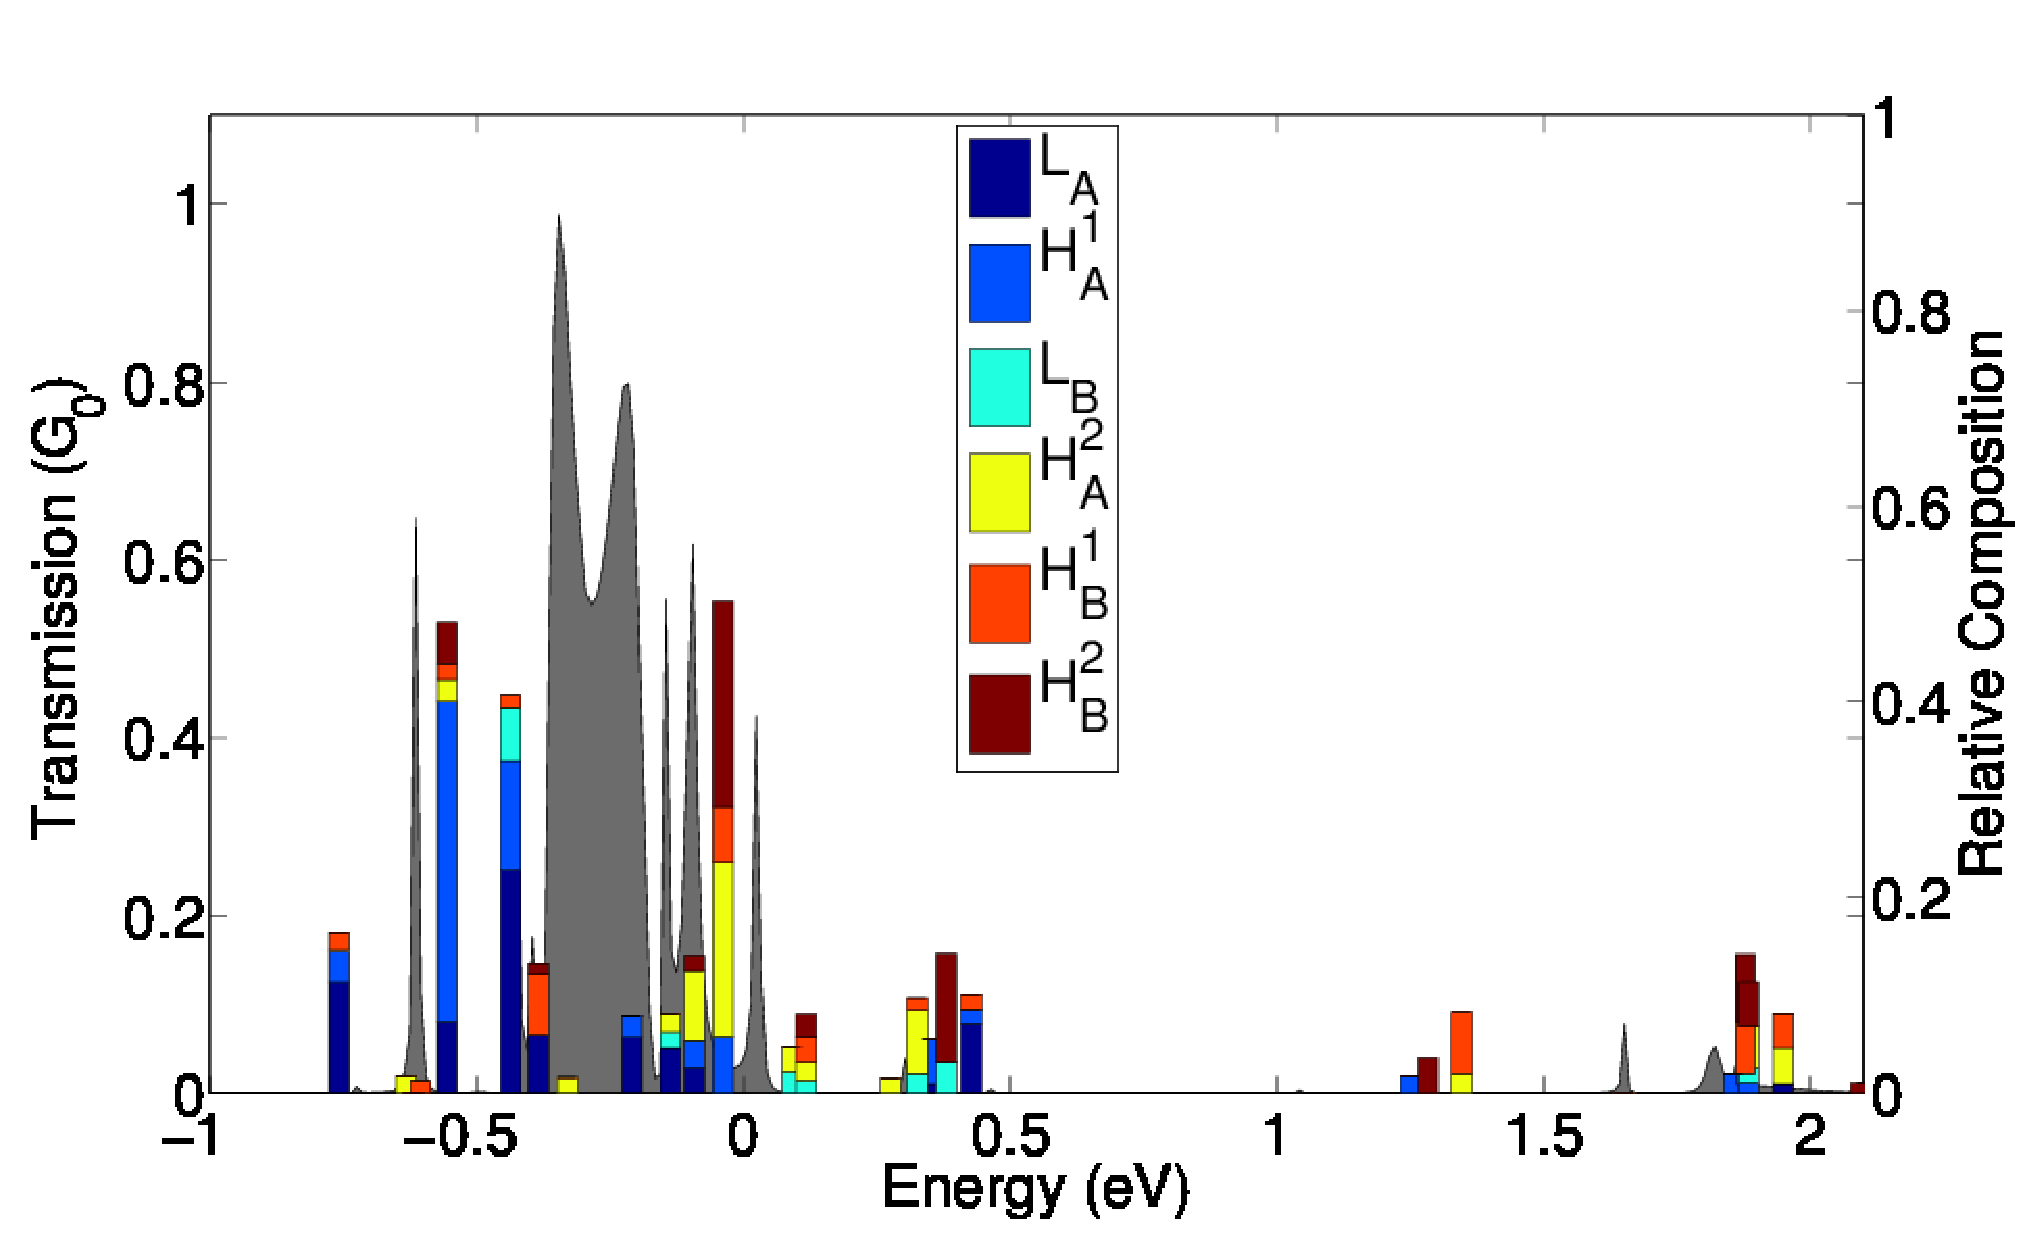
\includegraphics[width=\columnwidth]{img/ZnTPPdT/ZnTPP_peaks2}\label{fg:gaplevels}
   }
\caption{(a) Composition of peaks in transport, constructed by projection onto fragment molecular orbitals. A state with value 1 is a decoupled state, and completely un-hybridized (\eg HOMO-4 through --7), while HOMO-1, --2 and HOMO are strongly hybridized with each other \emph{and} the Au electrodes (reflected in their 30-50\% representation in the junction levels, with the rest originating from Au). The LUMO and LUMO+1 peaks are likewise strongly mixed with each other, coupling much less to the Au, reflected in the much narrower transport peaks near $1.7$ eV. (a) As in (a) for the interface levels rather than for the molecular orbitals shown in (a). }\label{peak-compositions}
\end{figure}

%\begin{figure}
% \subfloat[Hybridized HOMO for $(N+1)e$ in Junction]{
%   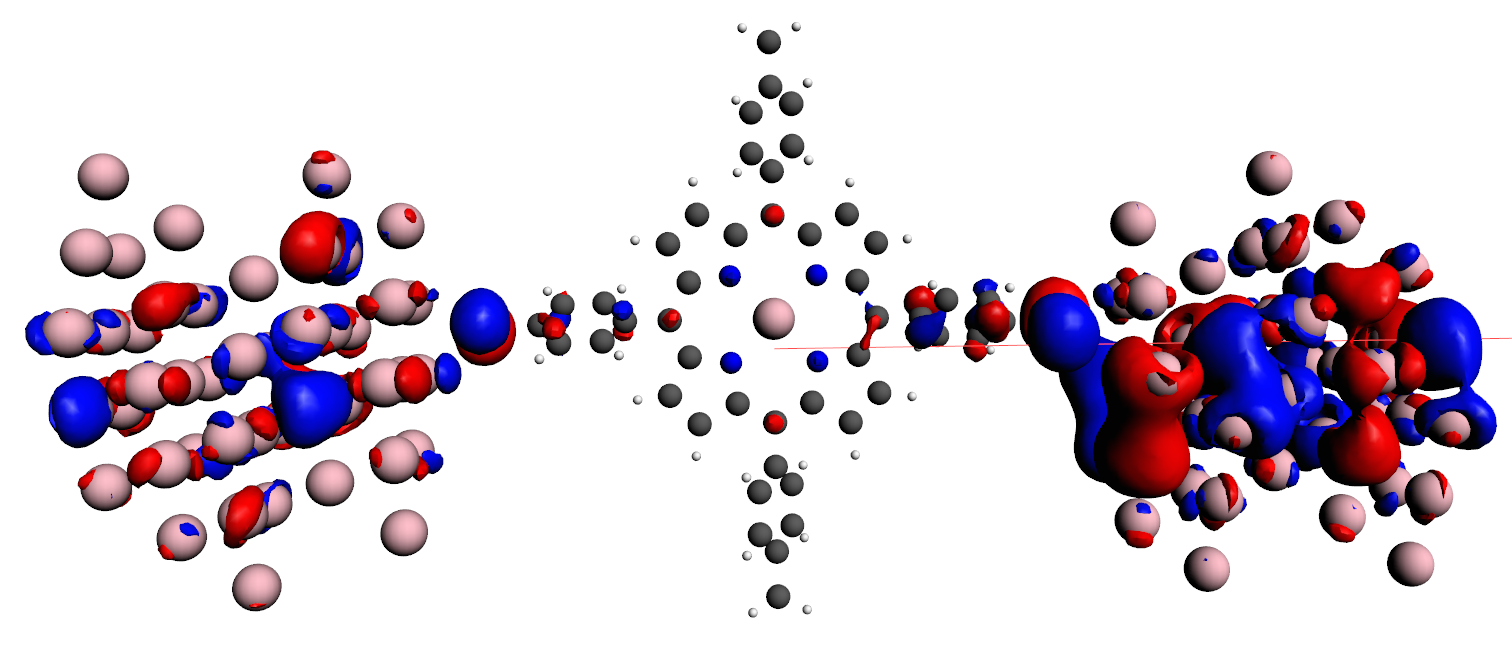
\includegraphics[width=.9\columnwidth]{img/ZnTPPdT/mVg_626.png}
%   \label{fg:zntpp-homo1}
% }\\
%  \subfloat[Hybridized HOMO in MCBJ geometry]{
%   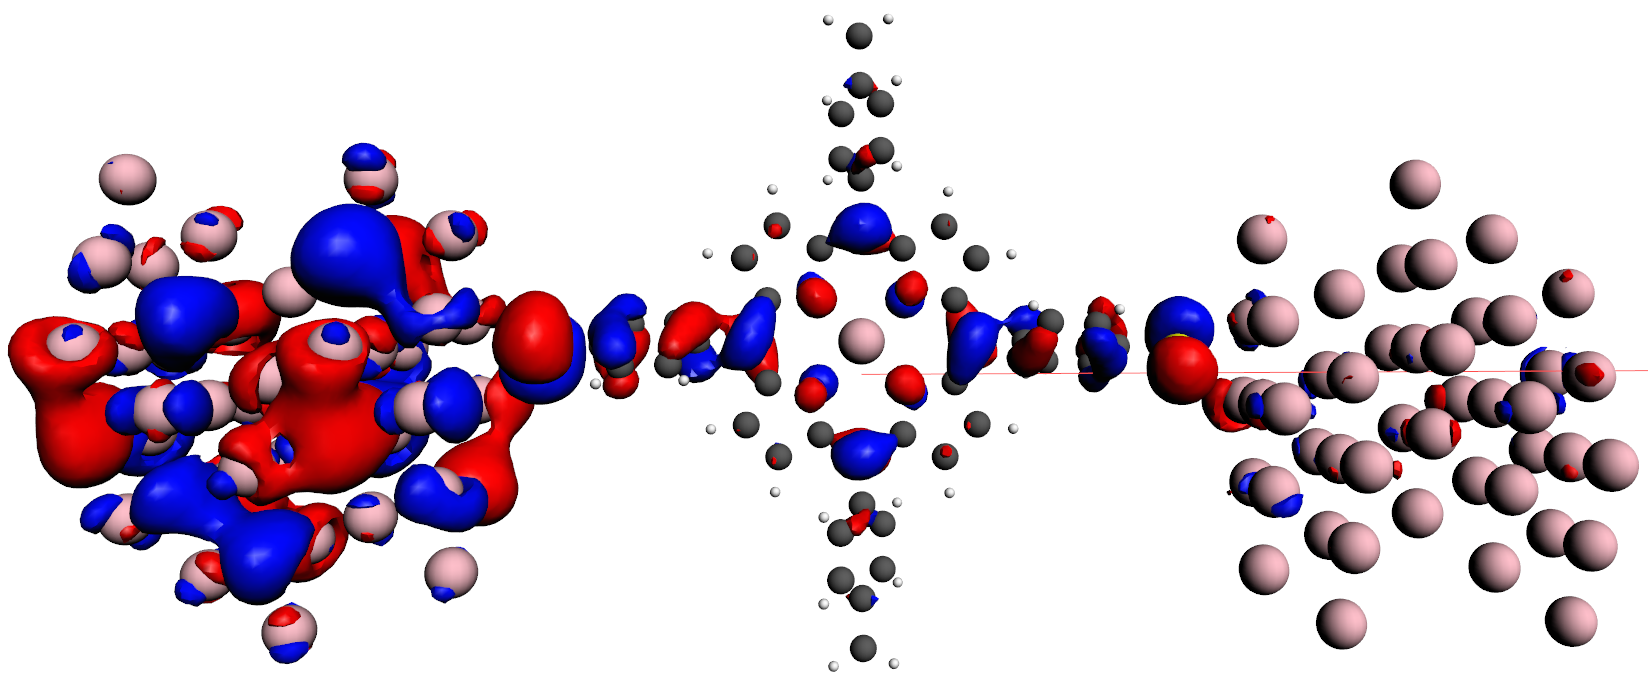
\includegraphics[width=.9\columnwidth]{img/ZnTPPdT/base_626.png}
%   \label{fg:zntpp-homo2}
% }\\
% \subfloat[Hybridized HOMO for $(N-1)e$ in Junction]{
%   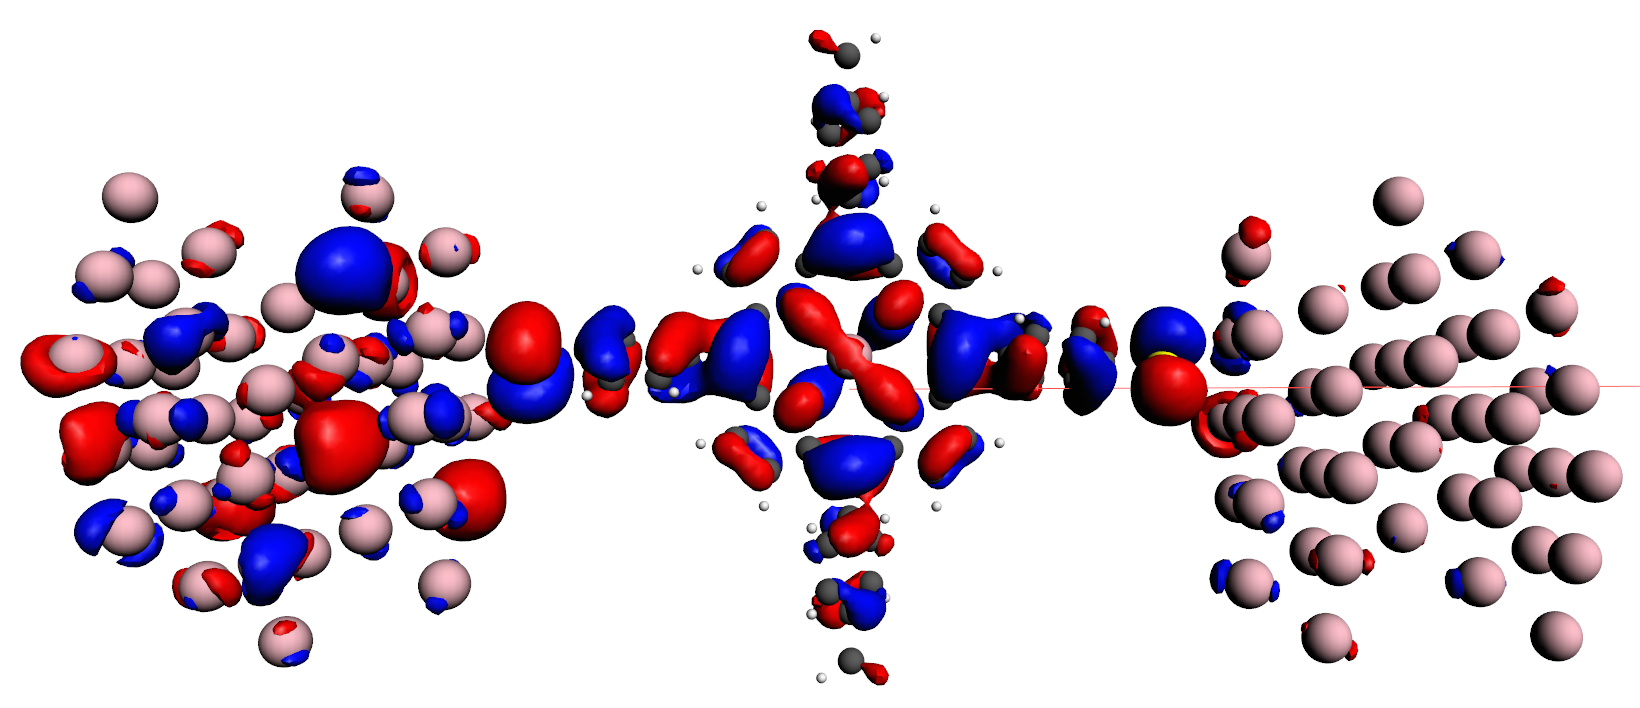
\includegraphics[width=.9\columnwidth]{img/ZnTPPdT/pVg_626.png}
%   \label{fg:zntpp-homo3}
% }

%\caption{Hybridization in the Au-ZnTPPdT junction: effective HOMO levels relative to the Fermi energy, gated such that (a) is the HOMO when there are roughly $N+1$ electrons on the molecule in the junction (interface state-like), (b) roughly $N$ electrons (HOMO-like, reference state has $V_g=0$ eV, net charge is $-0.05e$ but $+0.29e$ on the molecule excluding the negative thiols, see Fig.~\ref{fg:gated_charges}) and (c) roughly $N-1$ electrons (also HOMO-like, as HOMO is double occupied in neutral ground-state).}\label{fragment-hybridization}
%\end{figure}

\begin{figure}
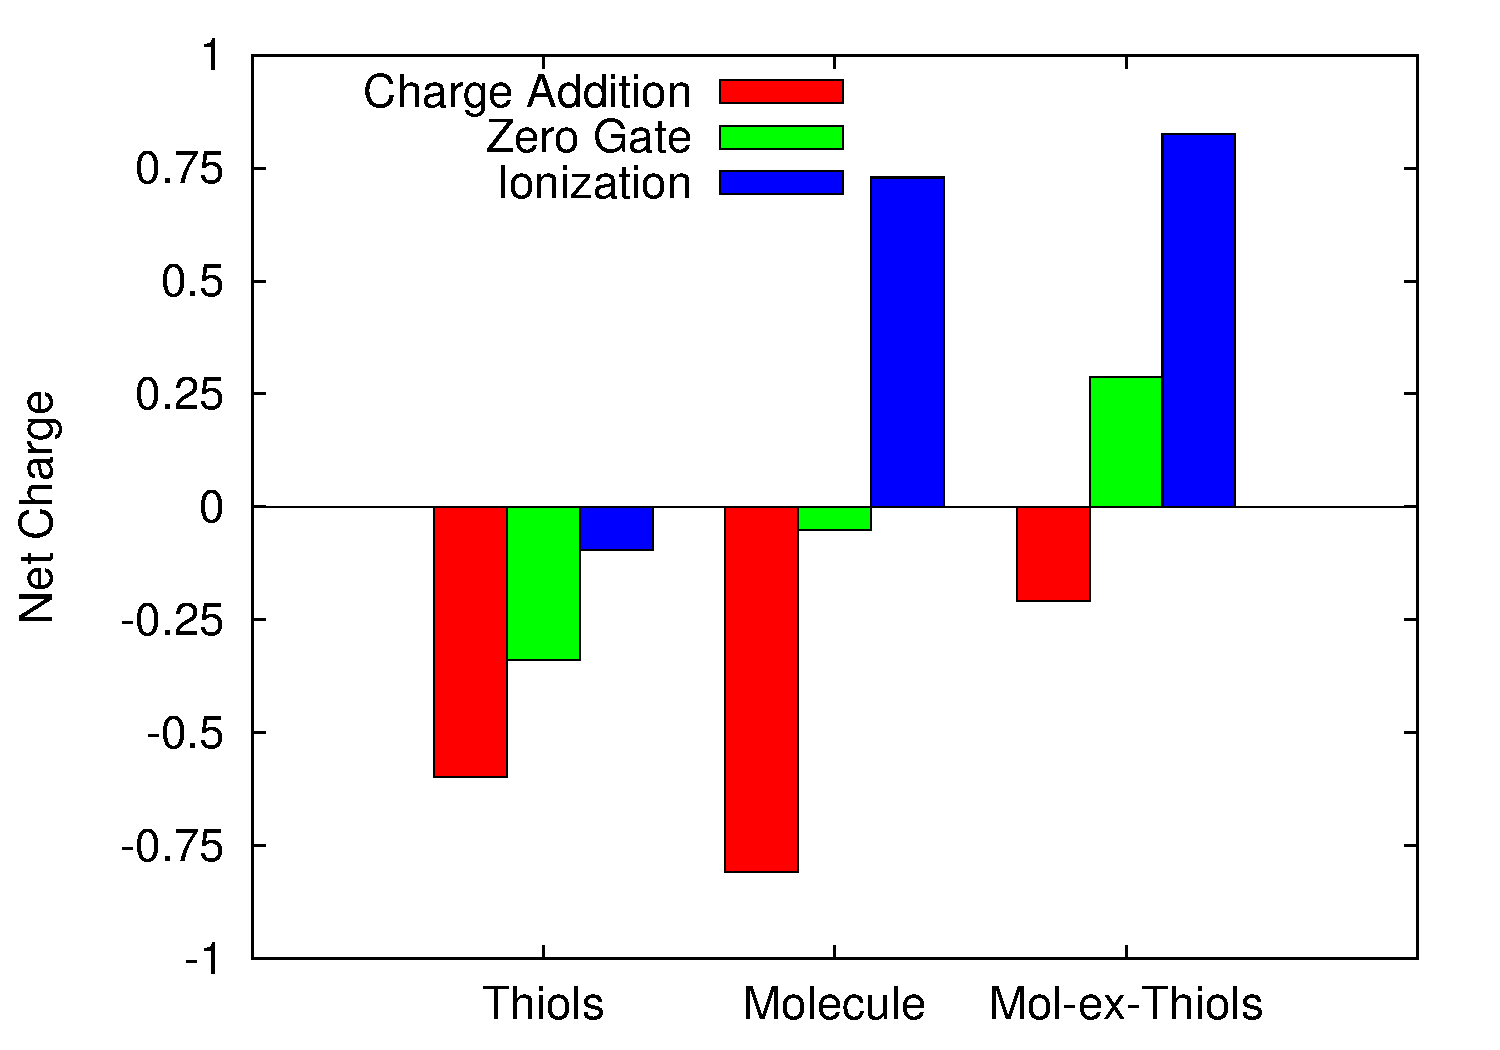
\includegraphics[width=.9\columnwidth]{img/gating}
\caption{Partial charges for the three gated transport levels (the reference state and gated such that the net charge is $\approx\pm e$), showing the difference in charging the molecule, thiols and molecule-without-thiols as the gating is varied. At zero-field, the molecule is roughly neutral, with negative thiols and a positive core.} \label{fg:gated_charges}
\end{figure}

Fig.~\ref{peak-compositions} shows the transmission of a typical transport calculation for the MCBJ geometry. % of Fig.~\ref{fg:4geometries}c
%using a hollow-site binding 
% with a nearest neighbor Au-S distance of 3.08\AA.%, corresponding to a 2.59\AA\xspace offset from the electrodes in a $24.26$\AA\xspace gap. 
We observe a cluster of HOMO-like peaks near $\epsilon_f$ (defined as $0$ eV), some small peaks inside the gap near $0.4$ eV, and the nearly-degenerate LUMO and LUMO+1 around $1.7$ eV. Fig.~\ref{fg:decompositions}, shows the decomposition of the transmission into fragment orbitals directly corresponding to molecular orbitals, and in Fig.~\ref{fg:gaplevels} for the interface orbitals.

The peaks right below the Fermi level derive mostly from the HOMO,\footnote{Identified by analyzing the orbital symmetries of the wavefunctions of these levels.} with significant amounts of interface levels mixed in.
Fig.~\ref{fg:gaplevels} shows the role of the 6 interface levels labeled L$_\text{A,B}$, H$^1_\text{A,B}$ and H$^2_\text{A,B}$, derived from hybridization of HOMO and LUMO with the gold. 

%The charge density deviates most strongly from neutral near the interface due to the chemisorption-induced charge transfer. The hybridization associated with the chemisorption is responsible for the smearing of the sharp resonances of molecular levels into broader peaks in transport near $\epsilon_f$.

%The fact that the LUMO peak is about 1.7~V from the Fermi level makes it very unlikely that this plays a role in the transport measurements. 
%The interface states composing the peak around 0.35~V above $\epsilon_f$ are more likely to be responsible for transport peak associated with an 
%unoccupied level. This peak is composed mostly of H$^2_\txt{A}$ and H$^2_\txt{B}$. 
%
%Our conclusions from these calculations may be summarized as follows:
%\begin{itemize}
%\item It is unlikely that the LUMO level is available within the experimental bias-window of roughly $1.0$ eV, given that zero-bias transport is HOMO-dominated, as the LUMO resonance is found at $1.7$ eV above the Fermi energy in Fig.~\ref{peak-compositions}. A more accurate calculation of the EA with GGA and B3LYP functionals, taking energy differences between two calculations for charge states $N,N+1$ (\emph{i.e.} the $\Delta$SCF approach), yields values for the addition energy $IP-EA$ in the range of $1.8-2.7$ eV.
%
%\item The dominant spectral feature just above $\epsilon_f$ is due to the interface states, in particular H$^{2}_{A}$. Its presence in the transport suggest that these features are observed as unoccupied transport resonances in the experiment.
%
%\end{itemize}

We have applied our method for calculating image-charge effects to this junction. In the reference state the net charge is $-0.05e$ with a strongly negative charge ($-0.34e$) on the thiols, and $+0.29e$ on the rest of the molecule, mainly on the Zn ion. Figure~\ref{fg:NNpm1-charges} shows the 
difference in charge for the ionized ($N-1$) states with respect to the reference state. This difference 
resides mostly on the arms, increasing the image charge effect a lot due to the proximity of the extra charge to the contacts. 

\begin{figure}
 \subfloat[]{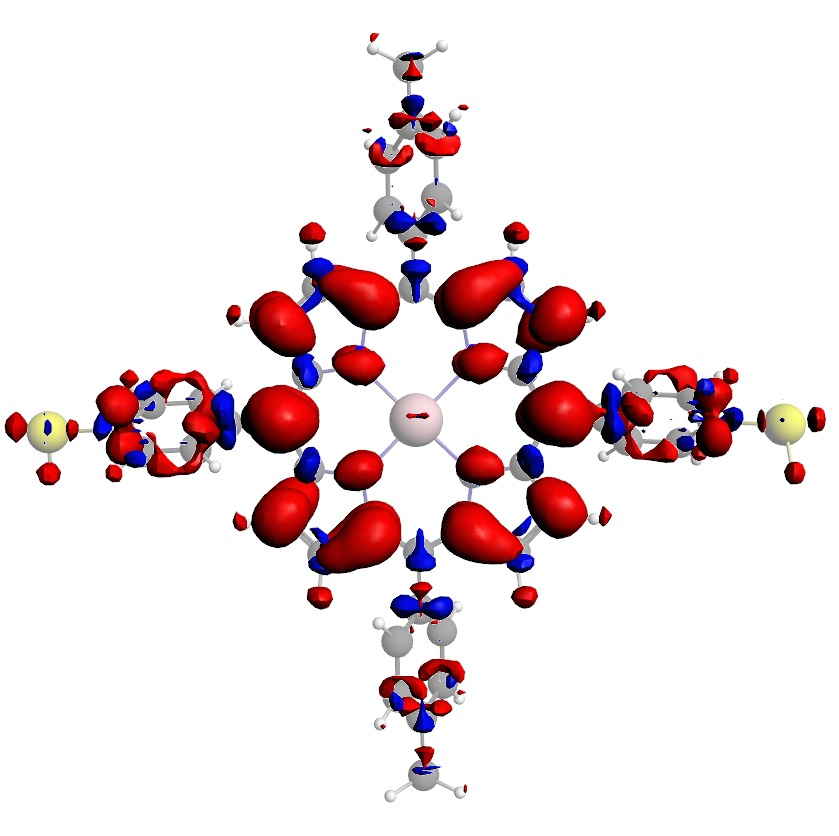
\includegraphics[width=.75\columnwidth]{img.exp/gas_charge}}\\
 \subfloat[]{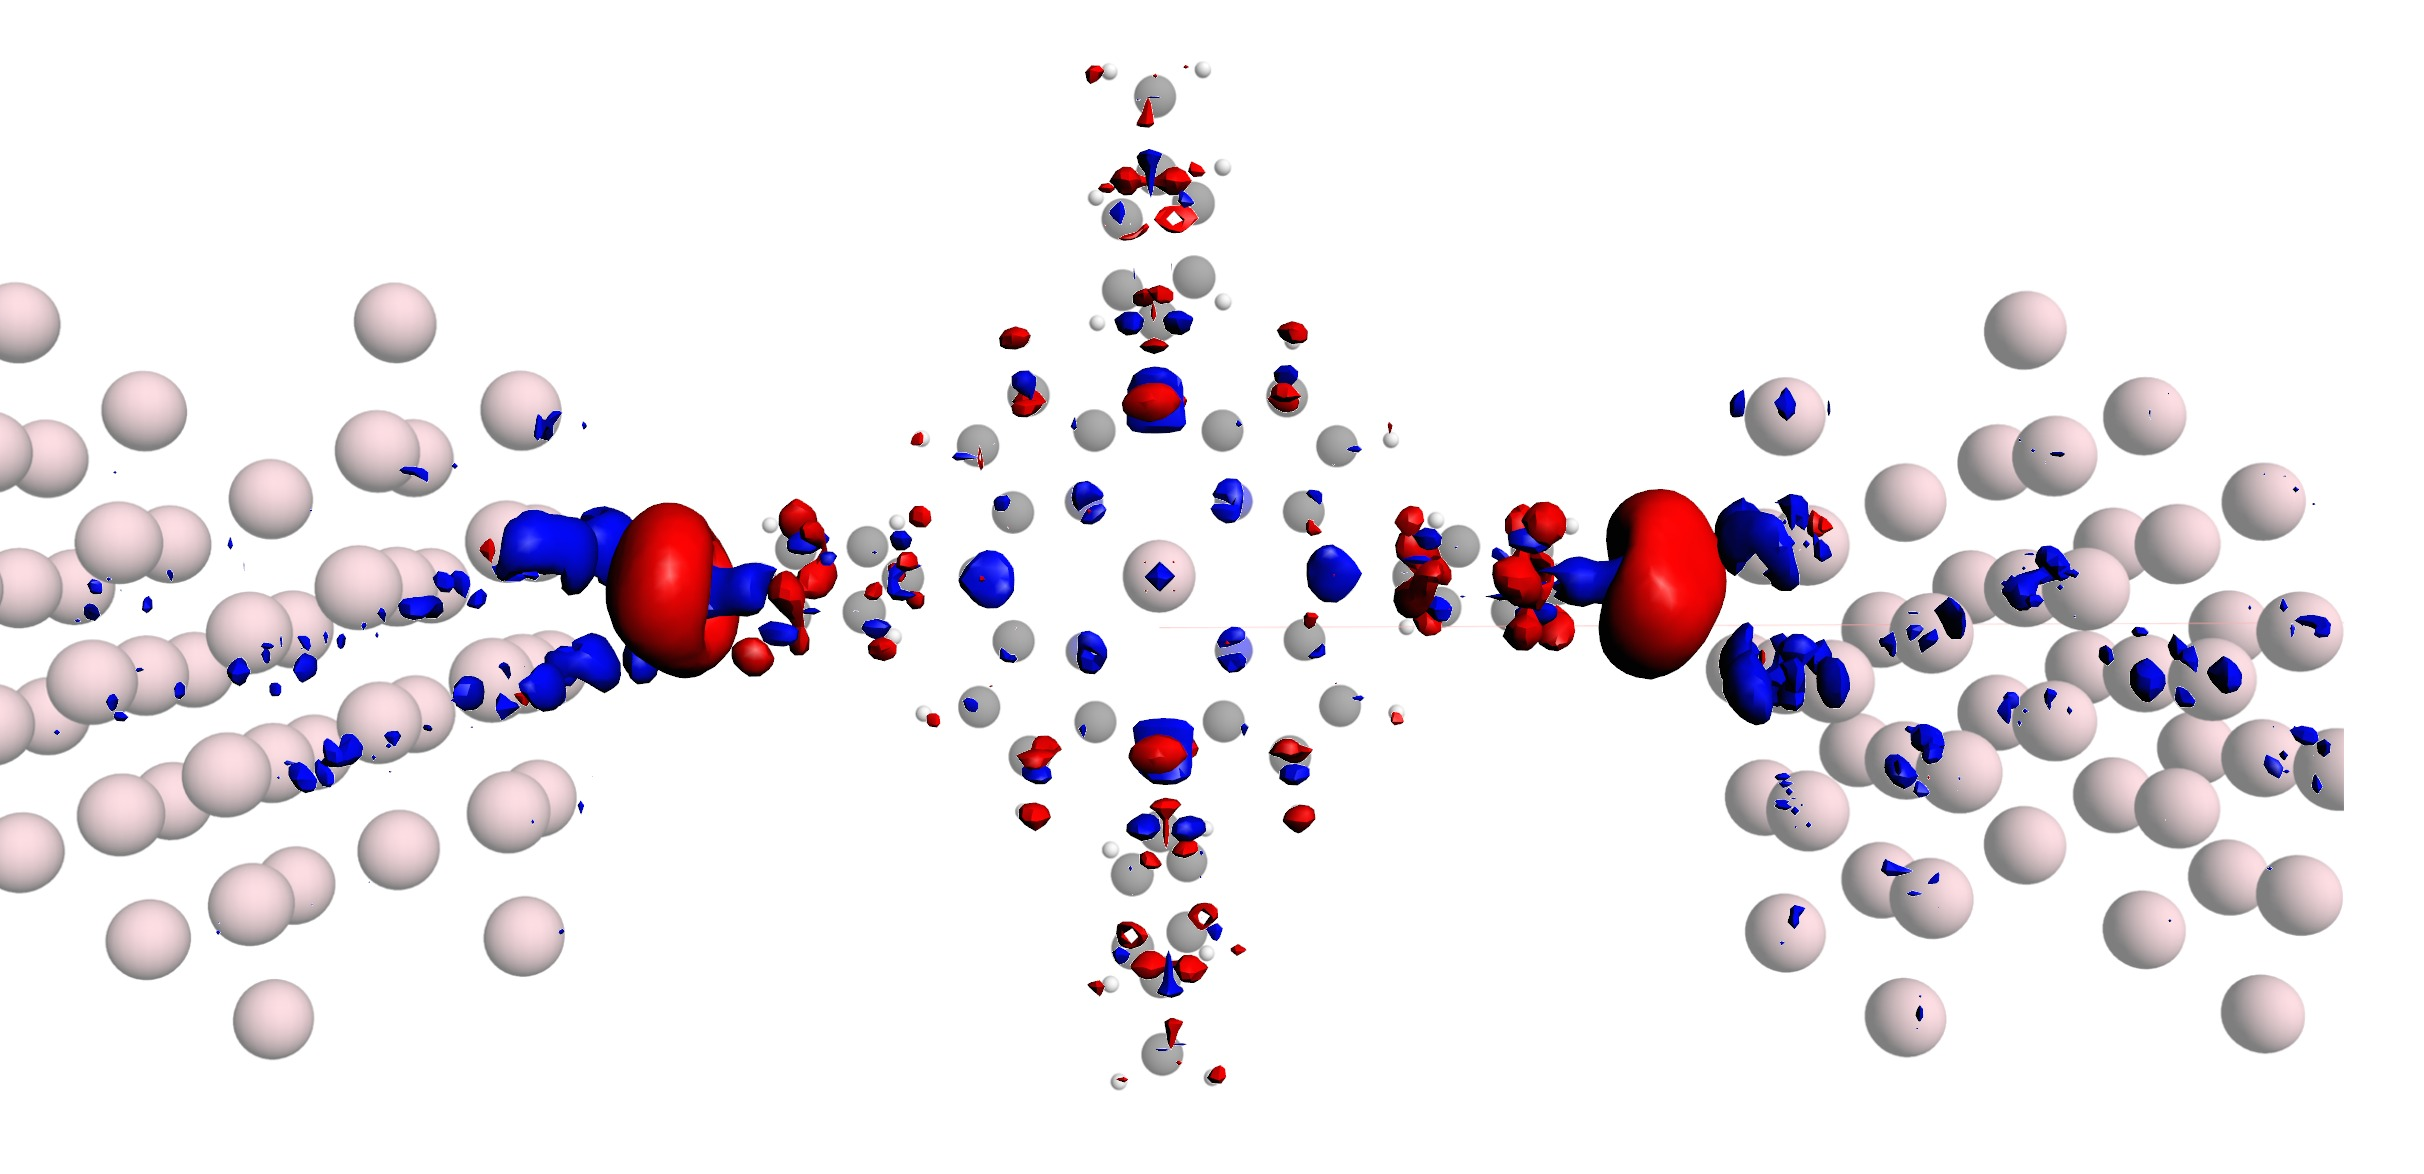
\includegraphics[width=\columnwidth]{img.exp/gate_charge}}
\caption{Difference in charge distribution in the $N+1$ relative to the $N$ electron charge states. Red indicates the increase of negative charge when adding an electron; blue the decrease. Differences for (a) gas phase DFT calculations (LUMO like difference) and (b) for gated DFT+NEGF transport calculations (recalling the interface levels of Fig.~\ref{fg:ZnTPP-frag}).} \label{fg:NNpm1-charges}
\end{figure}







%\subsection{Image-Model Calculations}\label{imagemodelcalcs}

The fact that in the reference state the molecule is slightly charged ($0.05e$), together with the importance of the interface states in the electron transport, suggest that the atomic charges in a junction geometry lead to image charge effects deviating significantly from those based on gas phase calculations.

\begin{figure*}
\subfloat[Geometry for Image-Charge Shifts]{
   \raisebox{0.8cm}{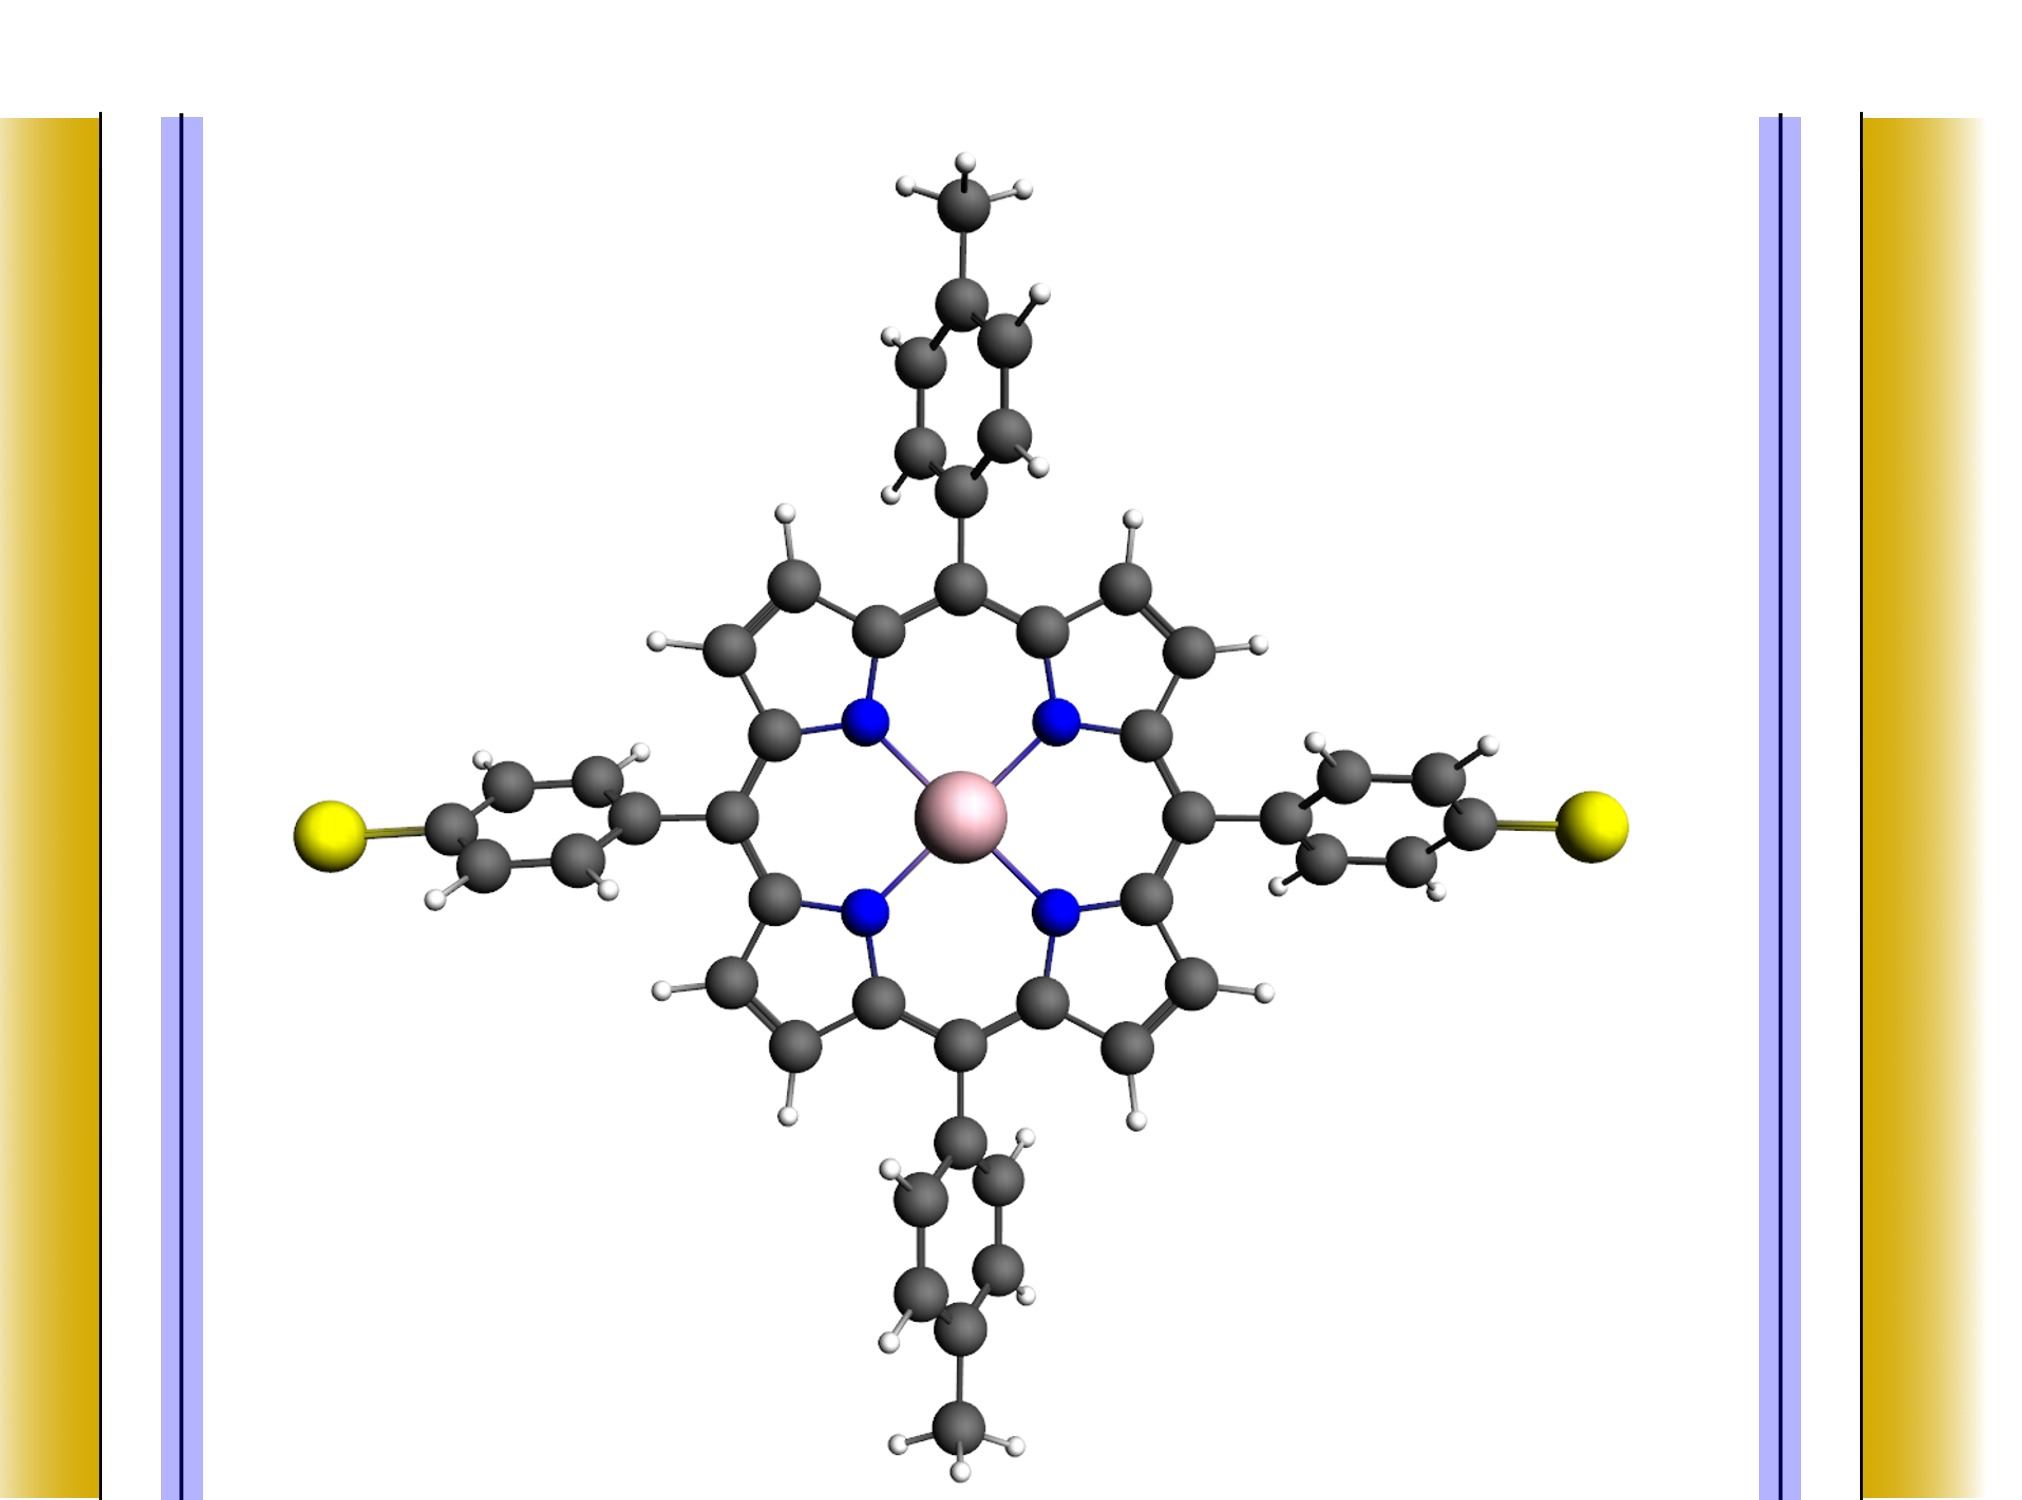
\includegraphics[width=.9\columnwidth]{img.exp/Simplified-Images}\label{fg:shiftsgeom}}
   }
\subfloat[Transport Gap Renormalization]{
   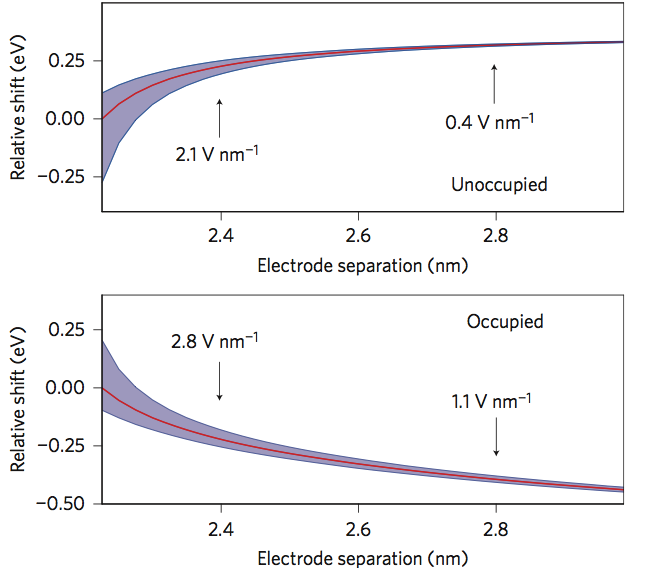
\includegraphics[width=.8\columnwidth]{img/SingleGapPlot3_eV}\label{fg:shiftscalc}
   }
\caption{
(a) Geometry used in the image-charge model, and (b) shifts predicted by the model (with uncertainties) showing the occupied- and unoccupied-levels both shifting towards $\epsilon_F$ with MGC's (the derivative with distance) in the range of $0.2-1.4$ eV/nm, expressed in the symmetrically applied bias. 
}\label{fg:Shifts}
\end{figure*}

%We apply the image model, by summing the electrostatic interactions for the molecule 
%between two parallel plates. 
The calculated level shifts as a function of distance are plotted in Fig.~\ref{fg:shiftscalc} 
Our calculations predict MGC's in the range of 
$1.1-2.8$ eV/nm for an occupied level and
$0.4-2.1$ eV/nm for an unoccupied level 
(in opposite directions), depending on the electrode separation (see Fig.~\ref{fg:shiftscalc}).
The different slopes differ significantly indeed, confirming the experimental findings. 

To obtain this difference, a detailed calculation of the molecule inside the junction is essential. Using gas-phase orbitals, the wrong orbital
(LUMO) would have been chosen as the unoccupied transport level, and the substantial contribution of the charge located at the arms of the hybridized 
HOMO would have been missed. 
%Fig.~\ref{fg:gas_vs_junction} compares the image-charge effects for the ZnTPPdT molecular junction with those calculated from atomic charges taken in gas phase. 
%The substantial difference between the two curves is more pronounced for smaller separations.

%Note that the sign of the rigid shift may be negative or positive, depending on the details of the charge distribution on the molecule. 

%\begin{figure}
%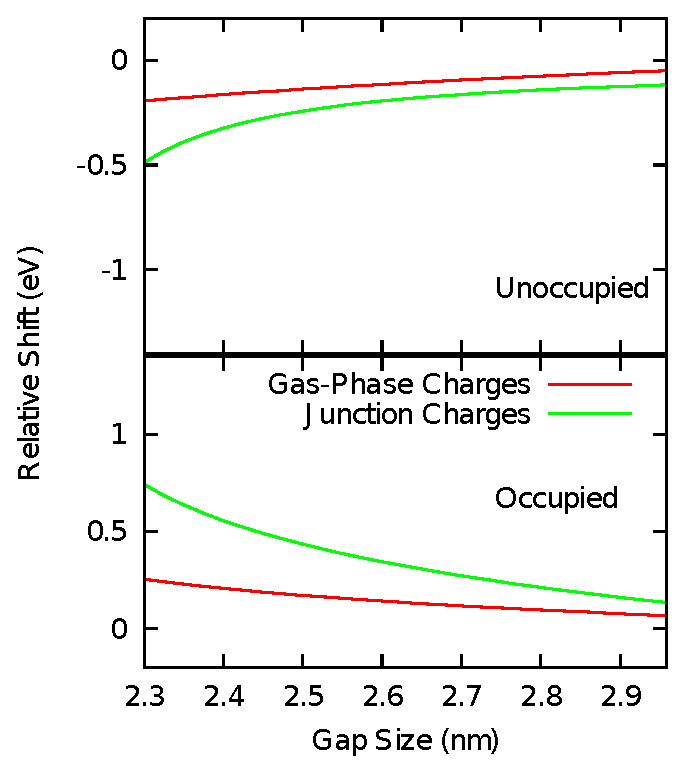
\includegraphics[width=.8\columnwidth]{img/Methods/Us_Gas_vs_Junction2}
%\caption{Comparison of results for total image-charge corrections using charges from gas phase calculations of ZnTPPdT and from ZnTPPdT in the molecular junction.} \label{fg:gas_vs_junction}
%\end{figure}

Our calculations reveal that the background image-charge effect contributes significantly to the MGC and explains the distance-dependent renormalization of the position of the molecular orbital levels with respect to the Fermi level of the electrodes. 
Taking the reference state to be the gas phase neutral state suppresses the asymmetry between the shifts for occupied and unoccupied levels. %as is clear from Fig.~\ref{fg:gas_vs_junction}.
This supports our conclusion that for the measurements of Fig.~\ref{fg:experiment} an interface-stabilized level of the fragment has lost some charge, as is suggested by the peak above the Fermi level in our transport calculations, and that this level is being addressed in electron transport through the unoccupied state.





\section{Conclusions}

In summary, we have presented a method for calculating the image-charge effects which change the alignment of the occupied and unoccupied levels in molecular devices with the Fermi levels of the electrodes. Our approach is based on the charge distribution of the molecule in the junction, in different charge states, using atomic point-charges. It is essential to use these rather than their gas phase equivalents for two reasons. First, the relevant charge states may have a different character in gas phase molecules and molecules in a junction, due to the formation of ``interface levels'' in the latter. These are stabilized by the metal-molecule interface, and have no counterpart in the gas phase. Second, unlike in the gas phase, the reference state in the junction (at zero bias and gate) can carry a net charge, which implies a significant contribution to the reduction of the metal work function upon chemisorption of a molecule.

We applied our method to a standard benzenediamine molecule and we found our results in good agreement with those obtained using Mowbray's \etal model. When we set aside their assumptions and use our model, we include features that are absent when the gas phase charges are used. 

Perrin \etal's\cite{Perrin2013} experiments on Au-ZnTPPdT reveal distance-dependent level shifts which are in agreement with our calculations. In this experiment, the fact that the reference state is non-neutral causes the MGC for occupied and unoccupied levels to be quite different. 
Our model agrees with the experimentally determined shifts within a factor of two.

Our approach demonstrates that for addressing image-charge effects within DFT, considering molecules in the junction is essential.

%\begin{acknowledgement}
\begin{acknowledgements}
The authors thank the financial support by the Dutch Foundation for Fundamental Research on Matter (FOM), the EU FP7 program under the ``ELFOS'' grant agreement and a grant by the Netherlands' National Computing Facilities Foundation, financed by The Netherlands Organization for Scientific Research (NWO). We also thank C.A. Martin, J.S. Seldenthuis, F. Grozema, R. Eelkema and J. van Ruitenbeek for fruitful discussions.
\end{acknowledgements}
%\end{acknowledgement}

\bibliography{Image-Effects-in-Transport-Calculations}




\clearpage
\appendix



\section{Computational Details}\label{computational_methods}

In the main text we discuss the results of both molecular Density Functional Theory (DFT) calculations, and transport calculations based on the Non-Equilibrium Green's Functions formalism in combination with DFT (NEGF+DFT).\cite{Meir1992,Datta2000} We have modeled the image effects using toy models implemented in Python, which take the results of these quantum chemical calculations as inputs.

All quantum-chemical calculations were performed using the ADF/Band package,\cite{Velde1991,Wiesenekker1991,Verzijl2012} originally developed by the Baerends group at the Free University of Amsterdam. The NEGF formalism for modeling transport has been implemented by us in the ADF/Band quantum chemistry package,\cite{Verzijl2012} and was used to obtain the conductance as a function of energy for representative junctions discussed. 

For BDA and ZnTPPdT calculations we use a TZP basis of numerical atomic orbitals on the molecule. The LDA and GGA PBE functionals were used to analyze BDA juctions, while in analyzing ZnTPPdT junctions we only use the LDA functional.

Results were converged to energy changes of less than $10^{-3}$ Hartree per step, together with energy gradients of less than $10^{-3}$ Hartree/\AA\xspace maximum and $<6.7\cdot 10^{-4}$ Hartree/\AA\xspace RMS.





\section{LDA vs GGA}\label{LDA-vs-GGA}

For BDA, we consider three different regions to apply the gate field, as shown in Fig.~\ref{fg:gates-BDA}. The first contains the entire Au-BDA-Au fragment; the second one only the molecule and the third one only the benzene ring. Then we tune the applied gate such that the electric charge of the molecule changes by $\approx e$. 

\begin{figure}
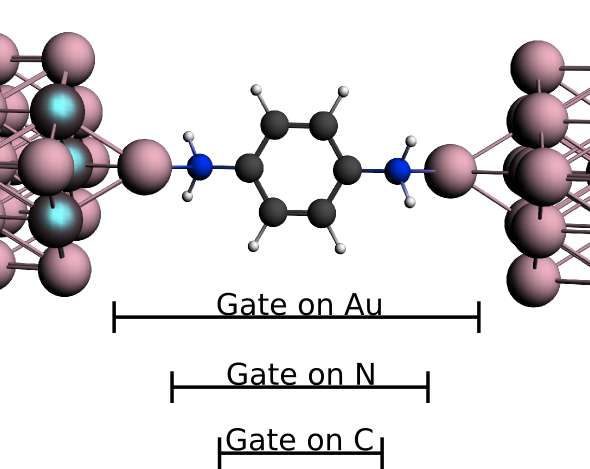
\includegraphics[width=0.85\columnwidth]{img.exp/BDA-Levels/gates.png} 
\caption{Three different regions where we applied the gate field, used to determine the position of the weakest coupling in the junction.}\label{fg:gates-BDA}
\end{figure}

We present the level shifts for LDA and GGA, for the gate on different parts of the junction (see Fig.~\ref{fg:shifts-gates}). We see that LDA and GGA are in good agreement. Furthermore, we conclude that the energy levels shifts are independent of the region where the gate field is applied and the use of LDA or GGA do not affect the results. 

\begin{figure}
\subfloat[LDA]{ 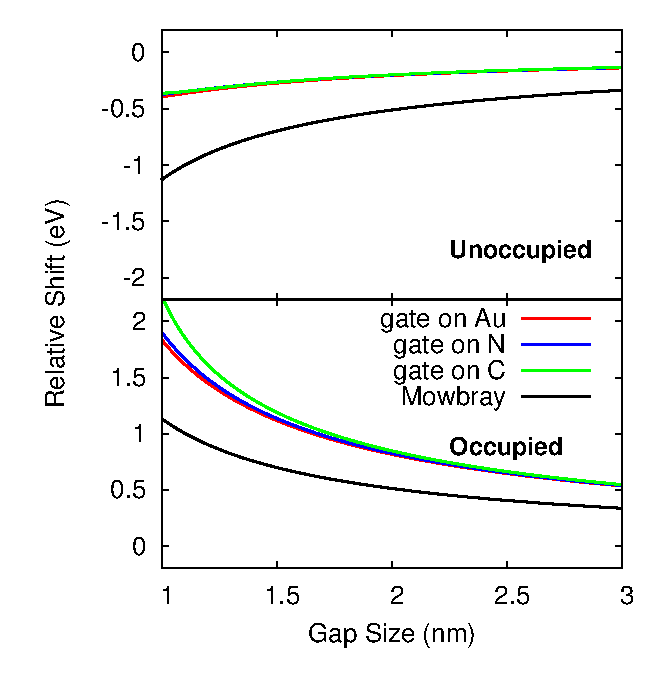
\includegraphics[width=0.5\columnwidth]{img/Us_vs_Mowbraygas_BDA-molecule-gates-LDA} }
\subfloat[GGA]{ 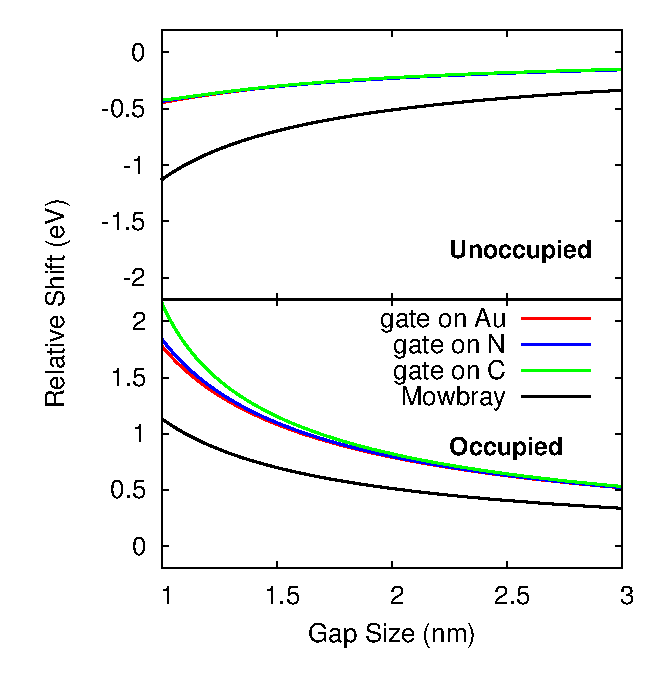
\includegraphics[width=0.5\columnwidth]{img/Us_vs_Mowbraygas_BDA-molecule-gates-GGA} }\\
\caption{Energy levels shifts for the BDA using (a) LDA in VWN parametrization, (b) GGA PBE functionals in our calculations.}\label{fg:shifts-gates}
\end{figure}

We also compare the atomic Hirschfeld charges obtained using the LDA/GGA for the exchange correlation energy (see table \ref{tab:charges}). Using the LDA functional, in the reference state, the charge of the molecule is equal to $+0.294e$ with approximately $+0.225e$ on the amines and $+0.069e$ on the rest of the molecule. These data in Fig.~\ref{fg:gated_charges_BDA} can be compared with those obtained using GGA in Fig.~\ref{fg:gated_charges_BDA-LDA}.


\begin{figure}
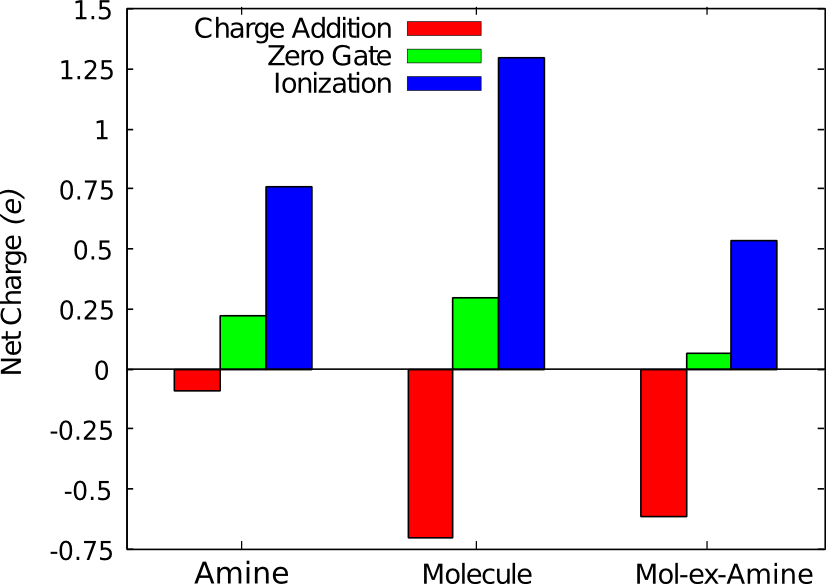
\includegraphics[width=.5\columnwidth]{img/gating-BDA-LDA-N}
\caption{Partial charges for the three gated transport levels (the reference state and $\approx\pm e$ charged), showing the difference in charging the molecule, amine groups and molecule-without-amine as the gate field is varied.} \label{fg:gated_charges_BDA-LDA}
\end{figure}

\begin{table}
\caption{Hirschfeld charge distribution obtained using LDA and GGA on BDA in the molecular junction with total q = +e and q = -e with respect to the reference state}\label{tab:charges}
\includegraphics[width=0.5\columnwidth]{img.exp/Fragment-geoms/nums-molecule.png} 
\scriptsize{
\begin{tabular}{c|ccc|ccc}
\hline\hline
  & \multicolumn{1}{c}{} & \multicolumn{1}{c}{LDA} & \multicolumn{1}{c|}{}
  & \multicolumn{1}{c}{} & \multicolumn{1}{c}{GGA} \\[1pt] \cline{2-7}
 %Atom &  & $Q$ &  &  & $Q$ &  \\
 Atom & q=-e & Ref. & q=+e & q=-e & Ref. & q=+e \\ \cline{1-7}
 1   & +0.084 & +0.129 & +0.182 & +0.080 & +0.123 & +0.177 \\ 
 2   & +0.084 & +0.129 & +0.182 & +0.081 & +0.123 & +0.177 \\ 
 3   & -0.218 & -0.146 & +0.015 & -0.209 & -0.140 & +0.021 \\ 
 4   & -0.028 & +0.021 & +0.077 & -0.028 & +0.022 & +0.077 \\ 
 5   & +0.019 & +0.070 & +0.104 & +0.010 & +0.062 & +0.095 \\ 
 6   & +0.021 & +0.072 & +0.105 & +0.011 & +0.063 & +0.096 \\ 
 7   & -0.161 & -0.067 & -0.012 & -0.161 & -0.063 & -0.007 \\ 
 8   & -0.161 & -0.066 & -0.011 & -0.160 & -0.063 & -0.006 \\ 
 9   & -0.160 & -0.065 & -0.009 & -0.159 & -0.062 & -0.005 \\ 
 10 & -0.159 & -0.065 & -0.008 & -0.158 & -0.060 & -0.004 \\ 
 11 & +0.020 & +0.071 & +0.105 & +0.011 & +0.063 & +0.096 \\ 
 12 & +0-021 & +0.072 & +0.105 & +0.012 & +0.064 & +0.097 \\ 
 13 & -0.023 & +0.026 & +0.081 & -0.023 & +0.026 & +0.080 \\ 
 14 & -0.219 & -0.148 & +0.012 & -0.210 & -0.140 & +0.018 \\ 
 15 & +0.088 & +0.130 & +0.183 & +0.084 & +0.125 & +0.178 \\ 
 16 & +0.089 & +0.131 & +0.184 & +0.085 & +0.125 & +0.178 \\ \hline\hline
\end{tabular}
}
\end{table}

A similar procedure was followed for ZnTPPdT. In section \ref{Sec:ZnTPP} we show LDA results, however GGA-level calculations with the PBE functionals do not qualitatively alter the results shown.

The resulting orbitals of the gas phase molecule are shown in Fig.~\ref{fg:ZnTPP-gas}, while the results for the fragment used in the transport calculations was previously shown in Fig.~\ref{fg:ZnTPP-frag}.

\begin{figure}
\subfloat[LUMO+1]{ \includegraphics[width=.35\columnwidth]{img.exp/ZnTPP-Levels/gas-phase/LUMO+1.png} }
\subfloat[LUMO]{ \includegraphics[width=.35\columnwidth]{img.exp/ZnTPP-Levels/gas-phase/LUMO.png} }\\
\subfloat[HOMO]{ \includegraphics[width=.35\columnwidth]{img.exp/ZnTPP-Levels/gas-phase/HOMO.png} }\\
\subfloat[HOMO-1]{ \includegraphics[width=.35\columnwidth]{img.exp/ZnTPP-Levels/gas-phase/HOMO-1.png} }
\subfloat[HOMO-2]{ \includegraphics[width=.35\columnwidth]{img.exp/ZnTPP-Levels/gas-phase/HOMO-2.png} }
\caption{Orbitals of gas phase ZnTPPdT}\label{fg:ZnTPP-gas}
\end{figure}






\end{document}
